%%%%%%%%%%%%%%%%%%%%%%%%%%%%%%%%%%%%%%%%%%%%%%%%%%%%
% Document type, global settings, and packages
%%%%%%%%%%%%%%%%%%%%%%%%%%%%%%%%%%%%%%%%%%%%%%%%%%%%

\documentclass[12pt]{report}   %12 point font for Times New Roman
\usepackage{graphicx}  %for images and plots
%\usepackage[letterpaper, left=1.5in, right=1in, top=1in, bottom=1in]{geometry}
\usepackage{setspace}  %use this package to set linespacing as desired
%\usepackage{times}  %set Times New Roman as the font
\usepackage[explicit]{titlesec}  %title control and formatting
\usepackage[titles]{tocloft}  %table of contents control and formatting
\usepackage[backend=bibtex, sorting=none, bibstyle=ieee]{biblatex}  %reference manager
\usepackage[bookmarks=true, hidelinks]{hyperref}
\usepackage[page]{appendix}  %for appendices
\usepackage[normalem]{ulem}  %for italicized text

% Jay adds these, non default
\usepackage{array}
\usepackage{subcaption}
\usepackage{amsmath}
\usepackage{color,soul}
\soulregister\cite7
\soulregister\ref7
\soulregister\pageref7
\usepackage[counterclockwise, figuresleft]{rotating}
\usepackage{placeins}

%%%%%%%%%%%%%%%%%%%%%%%%%%%%%%%%%%%
% Bibliography
%%%%%%%%%%%%%%%%%%%%%%%%%%%%%%%%%%%

%Add your bibliography file here
\bibliography{references}

% prevent certain fields in references from printing in bibliography
\AtEveryBibitem{\clearfield{issn}}
\AtEveryBibitem{\clearlist{issn}}

\AtEveryBibitem{\clearfield{language}}
\AtEveryBibitem{\clearlist{language}}

\AtEveryBibitem{\clearfield{doi}}
\AtEveryBibitem{\clearlist{doi}}

\AtEveryBibitem{\clearfield{url}}
\AtEveryBibitem{\clearlist{url}}

\AtEveryBibitem{%
  \ifentrytype{online}
    {}
    {\clearfield{urlyear}\clearfield{urlmonth}\clearfield{urlday}}}

%%%%%%%%%%%%%%%%%%%%%%
% Start of Document
%%%%%%%%%%%%%%%%%%%%%%

\begin{document}
\doublespacing  %set line spacing

%%%%%%%%%%%%%%%%%%%%%%%%%%%%%%%%%%%%%
% Title Page
%%%%%%%%%%%%%%%%%%%%%%%%%%%%%%%%%%%%%

%% Define your thesis title, your name, your school, and your month and year of graduation here

\newcommand{\thesisTitle}{Title of Your Thesis}
\newcommand{\yourName}{George P. Burdell}
\newcommand{\yourSchool}{Fiction}
\newcommand{\yourMonth}{January}
\newcommand{\yourYear}{1927}

%%%%%%%%%%%%%%%%%%%%%%%%%%%%%%%%%%%%%%%%%%%%%%%%%%%%%%%%%
% Do not edit these lines unless you wish to customize
% the template
%%%%%%%%%%%%%%%%%%%%%%%%%%%%%%%%%%%%%%%%%%%%%%%%%%%%%%%%%



\begin{titlepage}
\begin{center}

\begin{singlespacing}

\textbf{\MakeUppercase{\thesisTitle}}\\
\vspace{10\baselineskip}
A Dissertation\\
Presented to\\
The Academic Faculty\\
\vspace{3\baselineskip}
By\\
\vspace{3\baselineskip}
\yourName\\
\vspace{3\baselineskip}
In Partial Fulfillment\\
of the Requirements for the Degree\\
Doctor of Philosophy in the\\
School of \yourSchool\\
\vspace{3\baselineskip}
Georgia Institute of Technology\\
\vspace{\baselineskip}
\yourMonth{} \yourYear{}
\vfill
Copyright \copyright{} \yourName{} \yourYear{}

\end{singlespacing}

\end{center}
\end{titlepage}



\currentpdfbookmark{Title Page}{titlePage}  %add PDF bookmark for this page

%%%%%%%%%%%%%%%%%%%%%%%%%%%%%%%%%%%%%
% Approval Page
%%%%%%%%%%%%%%%%%%%%%%%%%%%%%%%%%%%%%

%% Define your committee members. If you have less than 6, simple delete/comment the unused lines

\newcommand{\committeeMemberOne}{Dr. Linda Wills, Advisor}
\newcommand{\committeeMemberOneDepartment}{School of Electrical and Computer Engineering}
\newcommand{\committeeMemberOneAffiliation}{Georgia Institute of Technology}

\newcommand{\committeeMemberTwo}{Dr. Lee Lerner, Advisor}
\newcommand{\committeeMemberTwoAffiliation}{Georgia Institute of Technology}

\newcommand{\committeeMemberThree}{Dr. Ayanna Howard}
\newcommand{\committeeMemberThreeDepartment}{School of Electrical and Computer Engineering}
\newcommand{\committeeMemberThreeAffiliation}{Georgia Institute of Technology}

\newcommand{\committeeMemberFour}{Dr. Patricio Vela}
\newcommand{\committeeMemberFourDepartment}{School of Electrical and Computer Engineering}
\newcommand{\committeeMemberFourAffiliation}{Georgia Institute of Technology}

\newcommand{\committeeMemberFive}{Dr. James Hamblen}
\newcommand{\committeeMemberFiveDepartment}{School of Electrical and Computer Engineering}
\newcommand{\committeeMemberFiveAffiliation}{Georgia Institute of Technology}

\newcommand{\approvalDay}{28}
\newcommand{\approvalMonth}{April}
\newcommand{\approvalYear}{2017}

%%%%%%%%%%%%%%%%%%%%%%%%%%%%%%%%%%%%%%%%%%%%%%%%%%%%%%%%%
% Do not edit these lines unless you wish to customize
% the template
%%%%%%%%%%%%%%%%%%%%%%%%%%%%%%%%%%%%%%%%%%%%%%%%%%%%%%%%%


\begin{titlepage}
\begin{singlespacing}
\begin{center}

\textbf{\MakeUppercase{\thesisTitle}}\\
\vspace{10\baselineskip}

\end{center}
\vfill

%Define minipages, depending on how many authors there are
\ifdefined\committeeMemberFour

Approved by:
\vspace{2\baselineskip}		%adjust the number in front of "\baselineskip" for alignment

\begin{minipage}[b]{0.4\textwidth}
	
	\committeeMemberOne\\
	\committeeMemberOneDepartment\\
	\textit{\committeeMemberOneAffiliation}\\
	
	\committeeMemberTwo\\
	%\committeeMemberTwoDepartment\\
	\textit{\committeeMemberTwoAffiliation}\\
	
	\committeeMemberThree\\
	\committeeMemberThreeDepartment\\
	\textit{\committeeMemberThreeAffiliation}\\
	
	\vspace{2\baselineskip}		%adjust the number in front of "\baselineskip" for alignment
	
\end{minipage}
\hspace{0.1\textwidth}
\begin{minipage}[b]{0.4\textwidth}
	
	\committeeMemberFour\\
	\committeeMemberFourDepartment\\
	\textit{\committeeMemberFourAffiliation}\\
	
	\ifdefined\committeeMemberSix
	\committeeMemberFive\\
	\committeeMemberFiveDepartment\\
	\textit{\committeeMemberFiveAffiliation}\\
	
	Date Approved: \approvalMonth{} \approvalDay, \approvalYear
	\vspace{1\baselineskip}		%adjust the number in front of "\baselineskip" for alignment
	
	\else
	
	\committeeMemberFive\\
	\committeeMemberFiveDepartment\\
	\textit{\committeeMemberFiveAffiliation}\\
		
	Date Approved: \approvalMonth{} \approvalDay, \approvalYear
	\vspace{5\baselineskip}		%adjust the number in front of "\baselineskip" for alignment
	
	\fi
	
\end{minipage}

\else

\hspace{0.6\textwidth}
\begin{minipage}[b]{0.4\textwidth}
	
	Approved by:
	\vspace{2\baselineskip}		%adjust the number in front of "\baselineskip" for alignment
	
	\committeeMemberOne\\
	\committeeMemberOneDepartment\\
	\textit{\committeeMemberOneAffiliation}\\
	
	\committeeMemberTwo\\
	\committeeMemberTwoDepartment\\
	\textit{\committeeMemberTwoAffiliation}\\
	
	\committeeMemberThree\\
	\committeeMemberThreeDepartment\\
	\textit{\committeeMemberThreeAffiliation}\\
	
	\vspace{2\baselineskip}		%adjust the number in front of "\baselineskip" for alignment
	
	Date Approved: \approvalMonth{} \approvalDay, \approvalYear
	\vspace{\baselineskip}		%adjust the number in front of "\baselineskip" for alignment
	
\end{minipage}

\fi





\end{singlespacing}
\end{titlepage}


%%%%%%%%%%%%%%%%%%%%%%%%%%%%%%%%%%%%%
% Epigraph
%%%%%%%%%%%%%%%%%%%%%%%%%%%%%%%%%%%%%

%% Define your quote and author for the epigraph here

\newcommand{\yourQuote}{``Are we recording? Is this thing on?''}
\newcommand{\yourAuthor}{George Washington}

%%%%%%%%%%%%%%%%%%%%%%%%%%%%%%%%%%%%%%%%%%%%%%%%%%%%%%%%%
% Do not edit these lines unless you wish to customize
% the template
%%%%%%%%%%%%%%%%%%%%%%%%%%%%%%%%%%%%%%%%%%%%%%%%%%%%%%%%%

\begin{titlepage}
\begin{center}

\vspace*{\fill}
\yourQuote\\
\textit{\yourAuthor}
\vspace*{\fill}

\end{center}
\end{titlepage}



%%%%%%%%%%%%%%%%%%%%%%%%%%%%%%%%%%%%%
% Dedication
%%%%%%%%%%%%%%%%%%%%%%%%%%%%%%%%%%%%%

%% Define your dedication statement here

\newcommand{\yourDedication}{A great dedication goes here.}

%%%%%%%%%%%%%%%%%%%%%%%%%%%%%%%%%%%%%%%%%%%%%%%%%%%%%%%%%
% Do not edit these lines unless you wish to customize
% the template
%%%%%%%%%%%%%%%%%%%%%%%%%%%%%%%%%%%%%%%%%%%%%%%%%%%%%%%%%

\begin{titlepage}
\begin{center}

\vspace*{\fill}
\yourDedication\\
\vspace*{\fill}

\end{center}
\end{titlepage}


%%%%%%%%%%%%%%%%%%%%%%%%%%%%%%%%%%%%%
% Acknowledgments
%%%%%%%%%%%%%%%%%%%%%%%%%%%%%%%%%%%%%

\pagenumbering{roman}
\addcontentsline{toc}{chapter}{Acknowledgments}
\setcounter{page}{5} % set the page number appropriately based on the number of intro pages
\clearpage
\begin{centering}
\textbf{ACKNOWLEDGEMENTS}\\
\vspace{\baselineskip}
\end{centering}

%Insert your dedication text here
Lorem ipsum dolor sit amet, consectetur adipiscing elit, sed do eiusmod tempor incididunt ut labore et dolore magna aliqua. Ut enim ad minim veniam, quis nostrud exercitation ullamco laboris nisi ut aliquip ex ea commodo consequat. Duis aute irure dolor in reprehenderit in voluptate velit esse cillum dolore eu fugiat nulla pariatur. Excepteur sint occaecat cupidatat non proident, sunt in culpa qui officia deserunt mollit anim id est laborum.

\clearpage
%\pagenumbering{gobble}  %remove page number on summary page


\addtocontents{toc}{\cftpagenumbersoff{chapter}} 

\currentpdfbookmark{Acknowledgments}{acknowledgments}
\addtocontents{toc}{\cftpagenumberson{chapter}} 

%%%%%%%%%%%%%%%%%%%%%%%%%%%%%%%%%%%%%
% Table of Contents
%%%%%%%%%%%%%%%%%%%%%%%%%%%%%%%%%%%%%

% Format for Table of Contents
\renewcommand{\cftchapdotsep}{\cftdotsep}  %add dot separators
\renewcommand{\cftchapfont}{\bfseries}  %set title font weight
\renewcommand{\cftchappagefont}{}  %set page number font weight
\renewcommand{\cftchappresnum}{Chapter }
\renewcommand{\cftchapaftersnum}{:}
\renewcommand{\cftchapnumwidth}{5em}
\renewcommand{\cftchapafterpnum}{\vskip\baselineskip} %set correct spacing for entries in single space environment
\renewcommand{\cftsecafterpnum}{\vskip\baselineskip}  %set correct spacing for entries in single space environment
\renewcommand{\cftsubsecafterpnum}{\vskip\baselineskip} %set correct spacing for entries in single space environment
\renewcommand{\cftsubsubsecafterpnum}{\vskip\baselineskip} %set correct spacing for entries in single space environment

%format title font size and position (this also applys to list of figures and list of tables)
%\titleformat{\chapter}[display]
%{\normalfont\bfseries\filcenter}{\chaptertitlename\ \thechapter}{0pt}{\MakeUppercase{#1}}

\renewcommand\contentsname{Table of Contents}

\begin{singlespace}
\tableofcontents
\end{singlespace}

\currentpdfbookmark{Table of Contents}{TOC}

\clearpage

%%%%%%%%%%%%%%%%%%%%%%%%%%%%%%%%%%%%%
% List of figures and tables
%%%%%%%%%%%%%%%%%%%%%%%%%%%%%%%%%%%%%

\addcontentsline{toc}{chapter}{List of Tables}
\begin{singlespace}
	\setlength\cftbeforetabskip{\baselineskip}  %manually set spacing between entries
	\listoftables
\end{singlespace}

\clearpage

\addcontentsline{toc}{chapter}{List of Figures}
\begin{singlespace}
\setlength\cftbeforefigskip{\baselineskip}  %manually set spacing between entries
\listoffigures
\end{singlespace}

\clearpage

%%%%%%%%%%%%%%%%%%%%%%%%%%%%%%%%%%%%%%%%%%%%%%%%%%%%%%%%%%%%%%%%%
% This is the Summary (abstract should be separate document)
%%%%%%%%%%%%%%%%%%%%%%%%%%%%%%%%%%%%%%%%%%%%%%%%%%%%%%%%%%%%%%%%%

\documentclass[12pt]{report}
\begin{document}

\clearpage
\begin{centering}
\textbf{SUMMARY}\\
\vspace{\baselineskip}
\end{centering}

\doublespacing

The motivation of this research is to provide a quantitative model for improving shadow detection in arbitrary environments. Many computer vision applications utilize the extraction of foreground pixels to capture moving objects in a scene; however, since shadows share movement patterns with foreground objects (and have a similar magnitude of intensity change compared with the background model), they tend to be extracted alongside the desired object pixels. Shadows generally contribute to inaccurate object classifications and impede proper tracking of foreground objects. Contemporary shadow removal algorithms have made great strides in discriminating between object pixels and shadow pixels, albeit with endemic limitations. In order to perform optimally, these leading methods require assumptions to be made about key factors of a scene, including illumination constancy, color content, clearly defined foreground objects, etc. As a result, no leading shadow removal methods are robust enough to compensate for a scene over time, nor are they suitable for deployment in an environment without a priori tuning of parameters. 
	
The objective of this research is to develop a framework capable of understanding salient scene parameters that affect shadow removal, and implement said shadow removal for an arbitrary scene for an arbitrary length of time.

\pagenumbering{gobble}  %remove page number on summary page
\end{document}


%%%%%%%%%%%%%%%%%%%%%%%%%%%%
%
% Chapters
%
%%%%%%%%%%%%%%%%%%%%%%%%%%%%

%%%%%%%%%%%%%%%%%%%%%%
% formatting
%%%%%%%%%%%%%%%%%%%%%%

% resume page numbering for rest of document
\clearpage
\pagenumbering{arabic}
\setcounter{page}{1} % set the page number appropriately

% Adjust chapter title formatting
%\titleformat{\chapter}[display]
%{\normalfont\bfseries\filcenter}{\MakeUppercase\chaptertitlename\ \thechapter}{0pt}{\MakeUppercase{#1}}  %spacing between titles
%\titlespacing*{\chapter}
%  {0pt}{0pt}{30pt}	%controls vertical margins on title
  
% Adjust section title formatting
%\titleformat{\section}{\normalfont\bfseries}{\thesection}{1em}{#1}

% Adjust subsection title formatting
%\titleformat{\subsection}{\normalfont}{\uline{\thesubsection}}{0em}{\uline{\hspace{1em}#1}}

% Adjust subsubsection title formatting
%\titleformat{\subsubsection}{\normalfont\itshape}{\thesubsection}{1em}{#1}

%%%%%%%%%%%%%%%%
% Chapter 1
%%%%%%%%%%%%%%%%

\clearpage

\def\bsq#1{
\lq{#1}\rq}

\chapter{Introduction}

The need for accurate video analytics has emerged in many application areas, including surveillance, transportation management, and smart-city sensing infrastructure. Many of these applications, e.g., pedestrian and traffic counting [\ref{Danner et al. ;) }], perform classification and analysis on moving objects. In order to detect and extract moving objects in an environment, foreground pixels are differentiated from those of the background through the use of statistical techniques, including Mixture of Gaussians, and Multi-Modal Mean [\ref{MoG}, \ref{MMM}]. These strategies establish a model of the background of a scene, which changes gradually over time. This background model is then compared directly to a frame. By finding the difference between an image frame and its background model, a mask containing the foreground pixels is created. Foreground pixels are then grouped together and segmented as a moving object, which is analyzed according to the needs of the application.

Applications that analyze moving objects rely on the accuracy of the foreground extraction of foreground pixels. These applications are disadvantaged by the fact that shadows are often mischaracterized as foreground objects, and are included as part of a moving object. This is often because shadows possess similar movement patterns and brightness compared to non-shadow foreground objects [\ref{Sanin -> others}]. Figure \ref{fig:nonshadow} illustrates the effect shadows have on the segmentation of foreground objects. 

\begin{figure}
  \centering
  \begin{subfigure}{.49\linewidth}
  \centering
  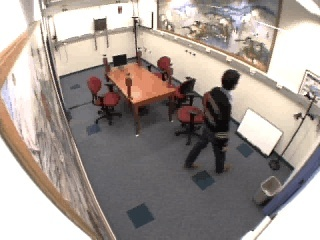
\includegraphics[width=1\linewidth]{figures/background/room_0295_frame.jpg}
  \caption{}
  \end{subfigure}
  \hfill
  \begin{subfigure}{.49\linewidth}
  \centering
  
\includegraphics[width=1\linewidth]{figures/background/room_0295_blob.jpg}
  \caption{}
  \end{subfigure}
  \hfill
  \begin{subfigure}{.49\linewidth}
  \centering
    
\includegraphics[width=1\linewidth]{figures/background/room_0295_shadows.jpg}
    \caption{}
  \end{subfigure}
  \hfill
  \begin{subfigure}{.49\linewidth}
  \centering
    
\includegraphics[width=1\linewidth]{figures/background/room_0295_clean.jpg}
    \caption{}
  \end{subfigure}
  %\caption{(a) Original frame, from the aton\_room dataset [\ref{ATON}]. (b) The foreground mask is provided, and segmented. Shadow pixels are shown in gray, and foreground object pixels in white. (c) Improper segmentation of the foreground due to shadows. (d) Proper segmentation with the removal of shadows.}
  \caption{The need for shadow removal: (a) Original frame from the aton\_room dataset [\ref{ATON}]. (b) Result of foreground extraction, with shadows incorrectly being detected as moving objects rather than as background. (c) Research goal: proper segmentation into shadow regions and true foreground. (d) Proper identification of foreground with the removal of shadows.}
\label{fig:nonshadow}
\end{figure}

The inclusion of shadows in foreground objects may hamper detection and tracking in several ways. Prominent issues, noted by Sanin et al. [\ref{Sanin}], include the distortion of an object's appearance model (required to properly track an object), and the erroneous joining of multiple objects into one labeled connected-component. Additional details regarding a shadow's effect on tracking can be found in [\ref{3,4 proposal?}]. The removal of shadows from foreground objects is thus a vital step in accurately segmenting moving foreground objects.

Classifying shadow pixels within moving foreground objects has been approached in numerous ways, including color-based attenuation models, geometric projective models, and texture-matching models [\ref{all these}, \ref{}, \ref{}]. Machine-learning has also been employed to attempt to learn the appearance of cast shadows in an unsupervised manner [\ref{Sato?}, \ref{Lee?}, \ref{Physical}]. A taxonomy of shadow removal methods produced by Prati et al. summarizes and evaluates four contemporary method classes: Statistical Nonparametric, Statistical Parametric, Deterministic Nonmodel-based and Deterministic Nonmodel-based [2]. The study concluded that the simpler methods were more suited for general practice, but ``to detect shadows efficiently in one specific environment, [adding] more assumptions yields better results.'' A second algorithm survey conducted by Sanin et al. in [1] evaluated more modern methods (catalogued as Chromacity, Geometry, Physical, Small Region Texture, and their own contribution, Large Region Texture) on the same datasets as above, yielding similar results concerning the generalization of shadow removal to an arbitrary scene. Mitra et al. provides a survey of threshold selection strategies for identifying shadows in moving foreground objects [3].

\section{The Problem}

These surveys indicate that existing shadow removal algorithms fail to optimally adapt to varying environmental properties; these methods quantifiably benefit from assumptions made about key factors of a scene, including illumination constancy, color content, and shadow intensity. In order to facilitate optimization, shadow removal methods possess algorithm parameters that are manually tuned to an environment. The reliance on environmental assumptions affects shadow removal in two ways: firstly, shadow removal performs suboptimally when deployed in an arbitrary environment, and secondly, even when manually calibrated, shadow removal fails to adapt to environmental parameters that change over time. From an application context, a surveillance system that monitors a sun-lit environment throughout an entire day will possess a wide range of shadow qualities when comparing shadows cast at dawn to shadows cast in the evening. Shadows cast in the same location may vary in darkness, size, orientation, and shape depending on the time of day. Therefore shadow removal must adapt not only to diverse environments, but continually adapt as environmental properties vary over time.

We quantitatively demonstrate several cases that indicate the need for adaptation. Shadow removal is judged by its detection rate and its discrimination rate, further detailed in section \ref{section:eval_metrics}. Detection rate indicates the number of shadow pixels correctly identified, while discrimination rate indicates the number of foreground object pixels that are correctly identified. Figure \ref{fig:coner1default} modifies a parameter belonging to Physical shadow removal, which controls the chromacity range in which a shadow can lie. The parameter (\textit{coneR1}) causes Physical shadow removal to perform optimally in the aton\_highway1 frame at a value of $0.2$. Similarly, the same algorithm performs poorly in the included dataset aton\_campus with the same parameter value. However, if \textit{coneR1} is modified from 0.2 to 0.68, aton\_highway1 experiences a 77\% loss of detection, while aton\_campus gains 53\% discrimination in exchange for a 15\% loss of detection (\ref{fig:coner168}). Geometry shadow removal was found to also showcase different results on the same scene, but with differing parameters (Figure \ref{fig:gweight}). 

% vthresh default
\begin{figure}
  \centering
  \begin{subfigure}{.49\linewidth}
    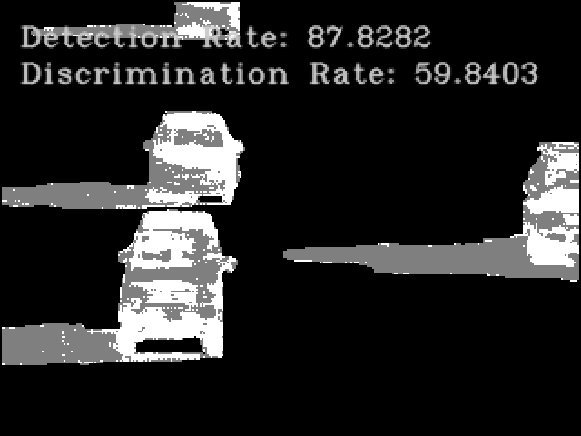
\includegraphics[width=1\linewidth]{figures/background/phys_highway1_200.png}
    \caption{aton\_highway1}
  \end{subfigure}
  \hfill
  \begin{subfigure}{.45\linewidth}
    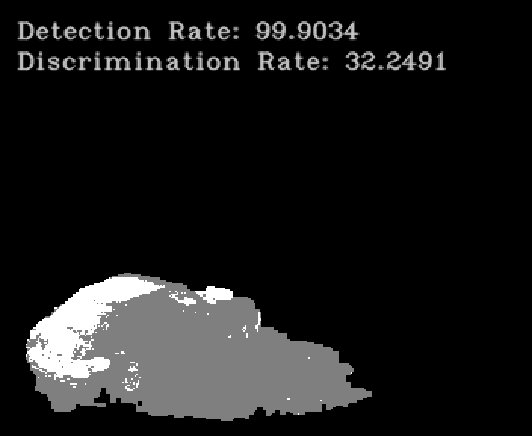
\includegraphics[width=1\linewidth]{figures/background/phys_campus_200.png}
    \caption{aton\_campus}
  \end{subfigure}
  \caption{\textit{coneR1} set to $0.2$. (a) Detection: 87.8, Discrimination: 59.84. (b) Detection: 99.9, Discrimination: 32.2}
  \label{fig:coner102}
\end{figure}

% vthresh15
\begin{figure}
  \centering
  \begin{subfigure}{.49\linewidth}
    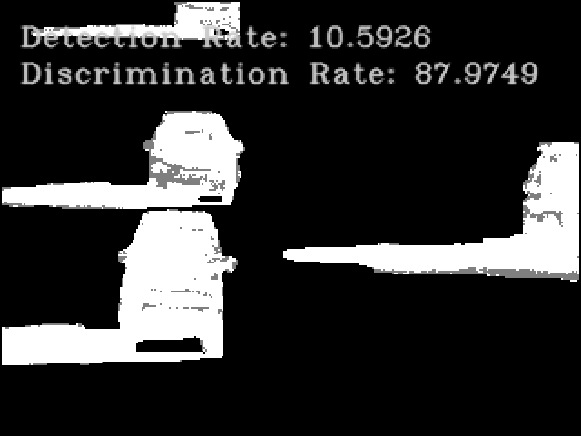
\includegraphics[width=1\linewidth]{figures/background/phys_highway1_680.png}
    \caption{aton\_highway1}
  \end{subfigure}
  \hfill
  \begin{subfigure}{.45\linewidth}
    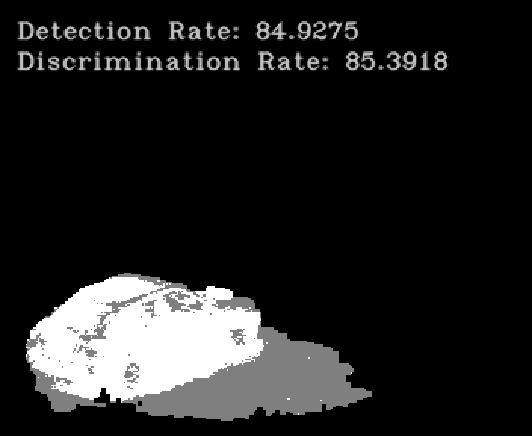
\includegraphics[width=1\linewidth]{figures/background/phys_campus_680.png}
    \caption{aton\_campus}
  \end{subfigure}
  \caption{\textit{coneR1} shifted from \bsq{0.2} to \bsq{0.68.} (a) Detection: 10.59, Discrimination: 87.97. (b) Detection: 84.9, Discrimination: 85.4. No parameter value provides consistent accuracy across datasets.}
  \label{fig:coner168}
\end{figure}

% gweight
\begin{figure}
  \centering
  \begin{subfigure}{.49\linewidth}
    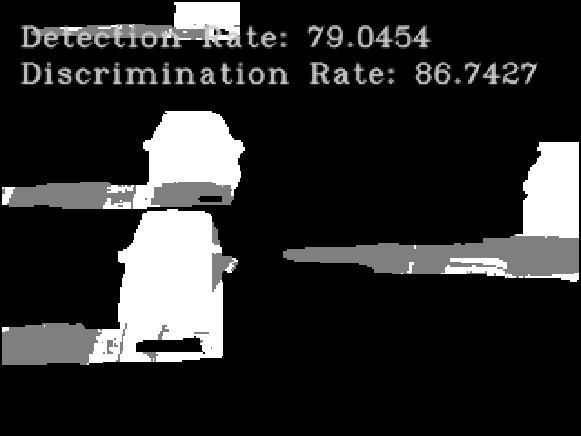
\includegraphics[width=1\linewidth]{figures/background/geo_highway1_70.png}
    \caption{\textit{gWeight: 70}}
  \end{subfigure}
  \hfill
  \begin{subfigure}{.49\linewidth}
    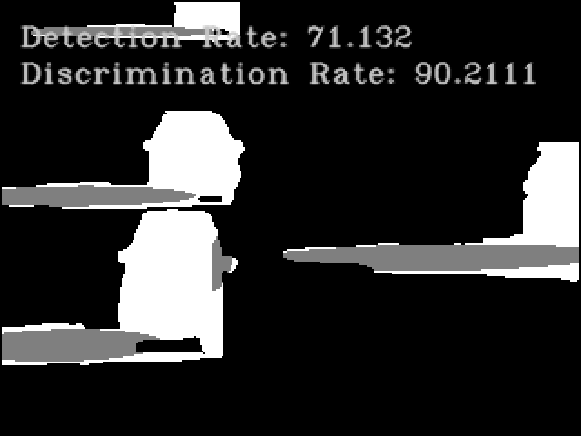
\includegraphics[width=1\linewidth]{figures/background/geo_highway1_0.png}
    \caption{\textit{gWeight: 0}}
  \end{subfigure}
  \caption{\textit{gWeight} shifted from '70' to '0.' (a) Detection: 79.05, Discrimination: 86.74. (b) Detection: 71.13, Discrimination: 90.21}
  \label{fig:gweight}
\end{figure}

%Precedent exists for intelligently adapting parameters for shadow removal. Sanin et al., in the implementation of Large Region Texture shadow removal, measure the average global attenuation, saturation, and foreground object perimeter of a scene. The algorithm selects several differing parameter values for hue, saturation, and value thresholds based on the average shadow attenuation and saturation of the scene. It also modifies the texture differential radius needed to qualify a pixel as shadow based on the perimeter of the foreground object in question. Our research seeks to provide a fully scalable approach, however, as the thresholds established for switching between parameter sets remain empirically determined and coarse-grained.

%%%

\FloatBarrier
\section{Objective and Contributions}

%None of the shadow removal methods analyzed are robust enough to compensate for environmental changes over time, nor do they optimally perform in an environment without a priori calibration of algorithm parameters. 
Our research seeks to establish an understanding of environmental properties that affect shadow removal, and use that understanding to optimize shadow removal in an arbitrary environment. This is achieved by automatically calibrating an algorithm's parameters based on observed environmental properties. Furthermore, we seek to create an understanding of how these environmental properties change over time, in order to continuously adapt shadow removal algorithms. These objectives require the creation of an adaptive model that automatically configures a shadow removal method to optimally perform given the observed environmental properties.

Our research makes the following contributions. We perform a qualitative assessment of each algorithm's performance in various environments. We construct and utilize an interactive framework for evaluating the sensitivity of an algorithm with respect to its mutable parameters. We identify and quantify observed environmental properties, and correlate them to sensitive algorithm parameters. Finally, we demonstrate the construction of an adaptive model, capable of leveraging correlated environmental properties to automatically tune an algorithm's parameters. The demonstration is completed by constructing a proof-of-concept model for Physical shadow removal.

Our proof-of-concept adaptive model draws upon the correlation between brightness attenuation in shadow regions and one of the Physical algorithm's parameters, \textit{coneR1}. It improves shadow detection by up to 10\% and shadow discrimination by up to 28\% on a range of standard datasets from ATON and PETS [\ref{aton}, \ref{pets}]. Additional indirect environmental factors are found to modify the effectiveness of the adaptive model. Various brightness calculation methods are shown to influence attenuation correlation by 7\% to 20\%.
A study of low-contrast feature keypoints in a scene was shown to improve attenuation-correlation by up to 12\% in some environments.

The outline of this thesis is as follows. In Chapter 2, we detail the shadow removal algorithms utilized in this study, and outline the steps taken to produce an adaptive model. Chapter 3 assesses the shadow removal algorithms for their performance in diverse environments, as well as their sensitivity to parametric change. These assessments culminate in the construction of a proof-of-concept adaptive model for Physical shadow removal, using its \textit{coneR1} parameter. Chapter 3 also explores indirect environmental properties and their potential impacts on the performance of the adaptive model. Chapter 4 quantifies and discusses the results of the adaptive model, and the indirect environmental properties' effects on the model. Chapter 5 summarizes conclusions and future work.

%Characterization of a scene or environment is traditionally done with global parameters such as global hue, saturation, and value (HSV), or color variance. However, more scene properties are needed for proper identification of semantic scene content, needed for this	 research. The ‘gist’ of scene, proposed by Oliva et al. in [5], compares evaluations of the properties of scene, using low-level features and simple arrangement of volumetric forms. Similarly, in [6], Oliva et al. evaluates the content of a scene using shape modeling such as the openness, ruggedness, roughness, expansion of a scene, creating the ‘spatial envelope’ of a scene. Lowe et al. propose the scale-invariant feature transform (SIFT), which utilizes and identifies features of a scene that are robust to noise, illumination, distortion, and viewpoint [7]. Bayesian Scene Modeling, proposed by Fei-Fei et al., utilizes the ‘bag-of-words’ strategy, building a dictionary of codewords relevant to a scene via unsupervised machine learning [8]. This approach creates a ‘theme’ for a scene built upon these collected codewords, categorizing complex diverse scenes into 13 categories (highway, coast, mountain, etc). 

%There is precedent for intelligently adapting parameters for shadow removal. Sanin et al., in the implementation of Large Region Texture shadow removal, measure the average global attenuation, saturation, and foreground object perimeter of a scene. The algorithm selects several differing parameter values for hue, saturation, and value thresholds based on the average shadow attenuation and saturation of the scene. It also modifies the texture differential radius needed to qualify a pixel as shadow based on the perimeter of the foreground object in question.

%\section{Work Completed}

%The implementations of the various approaches came with hard-coded parameters that were found to be correspondent with the provided datasets. Prominent parameters include:

%There are many more mutable parameters that affect shadow removal efficacy, and again, a more complete taxonomy will be provided. 
%In order to then quickly evaluate the effect of modifying these in-built parameters, a graphical interface was created to adjust them during runtime and view the effects. The interface supports either entire sequences (e.g. video) or singular frames. The interface supports any of the aforementioned shadow removal methods. 

%Fig. 1. Graphical interface for permuting parameters.

%The graphical interface is a crucial development in terms precisely measuring each parameter's effect on a given scene. However, in order to study shadow removal in terms of adaptivity over time, a more procedural method was required. Courtesy of username ‘brofield’, SimpleINI (github.com/brofield/simpleini), licensed under MIT, allowed for creation of .ini files containing any given removal method's default parameters. The algorithms themselves were then modified to allow for runtime modifications to be made to these parameters, meaning a procedural, iterative approach to analysis was created. A python script capable of writing to this .ini file allows for rapid permutation of parameters and values.

%Develop holistic scene content understanding in order to select shadow removal method for the ‘macro’ stage of hypervisor program. A quantization of seemingly qualitative scene content is required to better select between shadow removal methods. Some of this scene content includes shadow orientation vs. foreground object orientation, pre-existing static scene shadows, foreground object classification, distinctiveness of foreground objects (color differences in particular), light source in a scene, and many more. Building up an understanding of these scene properties may also help with the ‘micro’ stage of the proposed framework.

%Develop understanding of how these scene/environment parameters change over time of day and between locales. Observation of how both the quantitative and qualitative scene parameters change over time is required to create the proposed adaptive framework. This step will be simple for things like shadow intensity and global saturation, but more difficult for aforementioned properties like static shadows and object classification.

%Create correlation between global scene/environment properties and shadow removal accuracy. This step represents the main experimental thrust of the proposed research detailed thoroughly in this research summary.

%Use the aforementioned correlation to build hypervisor program to deploy adaptive shadow removal in arbitrary scenes and environments. This will be done primarily in C++, using the OpenCV API.

%%%%%%%%%%%%%%%%
% Chapter 2
%%%%%%%%%%%%%%%%

\clearpage
\chapter{Approach}

This chapter details evaluation metrics, provides background on the surveyed shadow removal algorithms, and outlines our research methodology. In section \ref{section:eval_metrics}, we quantify the metrics used to evaluate the accuracy of shadow removal. Section \ref{section:removalmethods} provides background on the shadow removal algorithms examined in this study. Finally, our research approach is outlined in section \ref{section:approach}.

\section{Evaluation Metrics} \label{section:eval_metrics}

The efficacy of a shadow removal algorithm on a given frame is evaluated with the popular metrics \textit{Detection} ($\eta$) and \textit{Discrimination} ($\xi$) (Eqn. \ref{eqn:detection}, Eqn. \ref{eqn:discrimination}) [\ref{to wherever they originated}]. These measure how many shadow pixels are correctly identified, and how many foreground object pixels are correctly preserved, respectively. The metrics are calculated using true positives (TP) and false negatives (FN) of both foreground pixels and shadow pixels. Subscripts signify identifications on shadow pixels ($S$) or foreground pixels ($F$).

\begin{equation}
\eta = \dfrac{TP_{S}}{TP_{S} + FN_{S}} \label{eqn:detection}
\end{equation}

\begin{equation}
\xi = \dfrac{TP_{F}}{TP_{F} + FN_{F}} \label{eqn:discrimination}
\end{equation}

\section{Background: Shadow Removal Methods} \label{section:removalmethods}

We select five popular shadow removal algorithms for this study, named Chromacity, Physical, Geometry, Small-Region Texture, and Large-Region Texture. These shadow removal methods use differing techniques for identifying foreground shadow pixels. These techniques are color information (Chromacity), brightness attenuation (Physical), shadow shape (Geometry), and texture information (Small-Region Texture, Large-Region Texture). We used standardized implementations of the shadow removal methods, licensed under GPL v3+ and written in C++ [\ref{shadowssourceforge}]. 
%Standardized implementations of the shadow removal methods, including ground truths, backgrounds, and frames, are used courtesy of A. Sanin, C. Sanderson, B.C. Lovell (http://arma.sourceforge.net/shadows), licensed under GPL v3+ and written in C++.

\subsection{Chromacity}

\textit{Chromacity}, or \textit{hue}, represents the base color of a pixel, and is separable from brightness and saturation. Chromacity-based shadow removal methods maintain that a pixel, when covered by a shadow, loses luminosity (or brightness), while retaining its chromacity. This assumption is referred to as  color constancy, or linear attenuation. This study implements one such algorithm from Cucchiara et al. [\ref{gucciara}], implemented using the Hue-Saturation-Value (HSV) color representation. 

Cucchiara et al. observe a shadowed pixel in the foreground ($fg_{p}$) retains its hue when compared to the corresponding background pixel ($bg_{p}$), while losing saturation and intensity (value). In order to be considered a shadow, the hue, saturation, and value of $fg_{p}$ must fall within the pre-determined thresholds $\tau_{H}$, $\tau_{S}$, and [$\beta_{1}$, $\beta_{2}$] (Eqn. \ref{eqn:huethresh}, \ref{eqn:satthresh}, \ref{eqn:brightthresh}).

\begin{equation} \label{eqn:huethresh}
| fg_{p}(H) - bg_{p}(H) | \leq \tau_{H}
\end{equation}

\begin{equation} \label{eqn:satthresh}
fg_{p}(S) - bg_{p}(S) \leq \tau_{S}
\end{equation}

\begin{equation} \label{eqn:brightthresh}
\beta_{1} \leq \dfrac{fg_{p}(V)}{bg_{p}(V)} \leq \beta_{2}
\end{equation}

%The thresholds are optimized for the environment the algorithm is intended to be deployed to. 
The thresholds are optimized for the environment of the algorithm's intended application. Due to its reliance on curated thresholds, Chromacity shadow removal is sensitive to strong illumination changes. Furthermore, the assumed linear attenuation model performs worse with dark shadows. 

\subsection{Physical}

For a shadow pixel to attenuate linearly, the light source casting the shadow must consist of primarily white light. Many environments experience multiple light sources, whether they are the sun, surface reflections, or blue light refracted from the sky. The presence of non-white light sources causes non-linear attenuation from a foreground shadow pixel to its background pixel.

This study uses an implementation of Cheng et al.'s Physical shadow removal, which attempts to learn the attenuation model of a shadow using a Gaussian Mixture Model (GMM) [\ref{Phys}]. Three features are used to learn the attenuation model of a pixel ($p$): illumination attenuation ($\alpha_{p}$), red-green direction ($\theta_{p}$), and blue direction ($\phi_{p}$). $\theta_{p}$ and $\phi_{p}$ are spherical coordinates, derived from the representation of the pixel $p$ as a vector $\vec{v}_{p}$ in the RGB coordinate plane. $\vec{bg}_{p}$ represents the pixel vector associated with the corresponding background model. Eqn. \ref{eqn:alphaatten}, Eqn. \ref{eqn:rgangle}, and Eqn. \ref{eqn:bangle} describe the calculation of these features.

\begin{equation} \label{eqn:alphaatten}
\alpha_{p} = \dfrac{||\vec{v}_{p}||}{||\vec{bg}_{p}||}
\end{equation}

\begin{equation} \label{eqn:rgangle}
\theta_{p} = arctan(\dfrac{\vec{v}_{p}(G)}{\vec{v}_{p}(R)})
\end{equation}

\begin{equation} \label{eqn:bangle}
\phi_{p} = arccos(\dfrac{\vec{v}_{p}(B)}{||\vec{v}_{p}||})
\end{equation}

Physical shadow removal first uses a weak detector to identify candidate shadow pixels, calculates the appropriate color features, and uses them to update the GMM. The GMM learns the attenuation model of a shadow over time, and is used to discriminate between foreground object pixels and shadow pixels.

\subsection{Geometry}

Widely-used Geometry-based shadow removal methods attempt to identify shadow regions in a foreground object using projective geometry [\ref{from sanin, mulitple}]. The implementation evaluated in this study, proposed by Hsieh et al. [\ref{Hsieh}], characterizes the geometric moments of foreground blobs in an attempt to identify the vertical peak and center of gravity of the objects. Using this information, the foreground object is split into an object region and a shadow region.

Geometric removal methods often require that a shadow and an object retain a clear orientation in regard to one another. Geometric removal is best deployed in environments with distinct, upright objects with a strong directional source of light.  

\subsection{Small-Region Texture}

Texture-based shadow removal attempts to match shadow pixels based on the underlying background texture, i.e., structural patterns observed in both the background model and the foreground. If similar structural patterns are observed, it is concluded that the foreground region does not occlude the background, and is therefore more likely to be a cast shadow.

Small-Region Texture (SRT) shadow removal, proposed by Leone et al. [\ref{Leone}], utilizes a set of Gabor functions with various bandwidths, orientations, and phases. A set of candidate shadow pixels, determined by a weak detector similar to that of Physical removal, is projected onto the set of Gabor filters. After analyzing both foreground and background, the texture correlation is found by computing the Euclidean distance.

\subsection{Large-Region Texture}

Large-Region Texture (LRT) shadow removal recognizes that the small regions analyzed using SRT may fail to contain enough structural information to match foreground to background. LRT takes advantage of Chromacity removal to produce regions of probable shadow candidates, and correlates the gradient information of both the foreground and background regions. LRT removal proves most effective in environments characterized by strong textural features and large contiguous shadow regions.

%The datasets used by Sanin et al. were also provided, and as such will be utilized in this research for more direct and accurate evaluations. The datasets vary in terms of environment, lighting, time of day, and actors of the scene. These different qualities lend themselves to be quite distinct from one another in terms of shadow length, color, orientation, and definition. Four datasets are indoors, and three outdoors. The spatial environments also differ in key factors such as background textures and color variances.

%%%
\section{Approach} \label{section:approach}
%%%

Our approach is divided into two components: algorithm assessment in the context of shadow removal in diverse environments, and the creation of the adaptive model for Physical shadow removal.

We first assess the previously catalogued algorithms (Chromacity, Physical, Geometry, SRT, and LRT removal) for sensitivity to both environmental and parametric change. We perform the analysis by applying each shadow removal method to each  environment represented by our datasets. The detection and discrimination rates of each method's shadow removal are plotted over time. Each method is judged based on its (detection/discrimination) response to the different environments of the datasets, and its response over time within each dataset.

We then perform a similar sensitivity analysis upon the parameters utilized by the algorithms. An algorithm is first explored through the use of 
%graphical tools, which enable simple understanding of a parameter's effect upon an algorithm. 
interactive graphical tools, which enable exploration of a parameter's 
effect upon an algorithm.  Parameter value ranges are also methodically 
swept to reveal the sensitivity of an algorithm's detection and 
discrimination rates to a give parameter's value.
%Parameters are also methodically iterated to illustrate a continuous relationship between a parameter's value and an algorithm's detection and discrimination rates.

From the sensitivity assessments, we demonstrate the creation of an adaptive model for Physical shadow removal's \textit{coneR1} parameter. We create this adaptive model as a proof-of-concept, demonstrating the capability of correlating environmental properties to an algorithm's parameter, and automatically calibrating the algorithm for improved shadow removal. The adaptive model is created in five steps:

%\begin{figure}
%  \centering
%  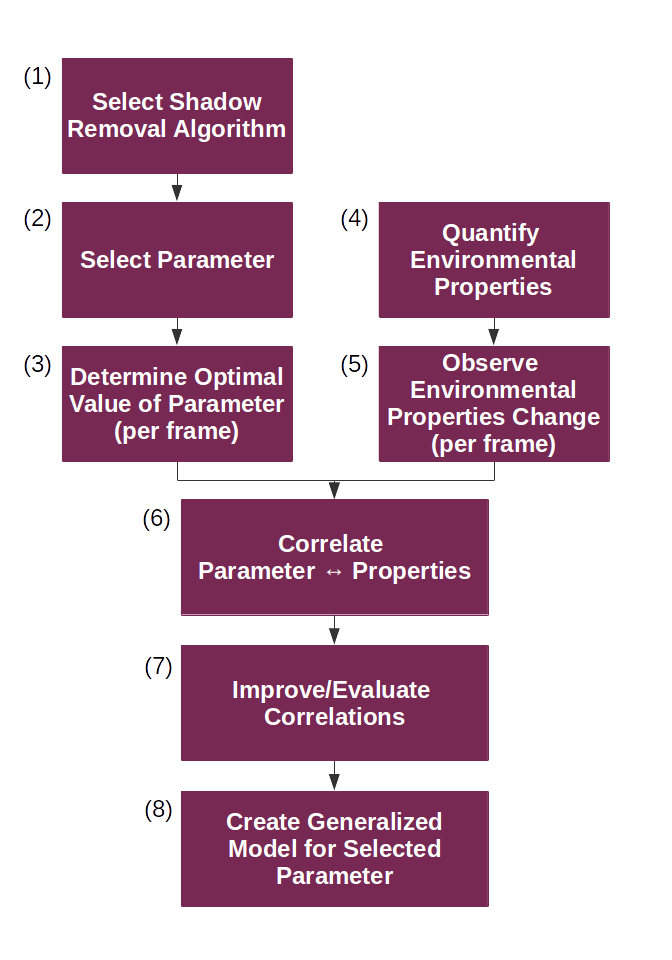
\includegraphics[width=.85\linewidth]{figures/background/overview.png}
%  \caption{Proof-of-concept overview.}
%  \label{fig:overview}
%\end{figure}

\begin{enumerate}
%\item \underline{Select Shadow Removal Algorithm}: The scope of the proof-of-concept model is restricted to one shadow removal algorithm. The algorithm selected must display reasonable sensitivity to both environmental changes. This proof-of-concept utilizes Physical shadow removal. Algorithm selection is detailed in section \ref{section:selectalgorithm}.

%\item \underline{Select Parameter}: In addition to demonstrating sensitivity to environmental change, the selected algorithm must also display sensitivity to parametric change. In section \ref{section:selectparameter}, we analyze multiple candidate parameters proven to significantly affect the accuracy of shadow removal.

\item \underline{Determine optimal value of parameter (per frame)}: In accordance with our sensitivity analysis, each frame of a dataset has an optimal value for the selected parameter, i.e., there is an optimal value for which shadow removal is maximized. The process for extracting these optimal values is detailed in section \ref{section:datacollection}.

\item \underline{Quantify environmental properties}: Observed environmental properties are the most influential factor for creating an adaptive model. Section \ref{section:envassess} details identifying and quantifying salient environmental properties. 

%\item \underline{Observe Scene Properties Change (per frame)}: Our adaptive model requires that an algorithm may adapt to arbitrary environments as well as environmental changes. Environmental properties' values are recorded for each frame of a dataset.

\item \underline{Correlate optimal parameter value and environmental properties}: For each dataset, optimal parameter values and environmental properties are recorded for each frame. By analyzing the correlation between the two sets, we receive a quantitative understanding of how well that environmental parameter would serve as the basis for an adaptive model. For example, if our optimal parameter value increases by $x\%$ from frame 1 to frame 2, and our environmental property also increases by $x\%$ from frame 1 to frame 2, that environmental property may be used to predict an appropriate value of our algorithm parameter. Consistent correlations are sought across each dataset to eliminate false positives.

\item \underline{Improve/evaluate correlations}: Many environmental properties exist that may not display direct correlation with a parameter's optimal value. We instead utilize these indirect properties as modulators to improve correlation observed with a primary environmental property. Multiple contributing environmental properties are combined to improve correlation and thereby shadow removal. Indirect properties are evaluated in sections \ref{section:nonlinearatten}, \ref{section:brightnessmodels}, and \ref{section:lowcSIFT}.

\item \underline{Create general model for selected parameter}: Incorporating direct and indirect correlative environmental properties, we construct an adaptive model capable of calculating a new value for the algorithm parameter that improves shadow removal. This model is independent of dataset, and is calculated per frame, rather than applied to every frame in a dataset. Methodology for building this model is found in section \ref{section:model}.
\end{enumerate}

%%%%%%%%%%%%%%%%
% Chapter 3
%%%%%%%%%%%%%%%%

\clearpage
\chapter{Methodology} \label{chapter:methodology}

This chapter contains the research methodology employed while implementing a proof-of-concept of an adaptive shadow removal model. Our methodology is divided into two components: algorithm assessment in the context of shadow removal in diverse environments, and the creation of the adaptive model for Physical shadow removal, one of the previously assessed algorithms.

We first assess the previously catalogued algorithms (Chromacity, Physical, Geometry, SRT, and LRT removal) for sensitivity to both environmental and parametric change. We then perform a similar sensitivity analysis upon the parameters utilized by the algorithms. These assessments are performed qualitatively to determine the feasibility of an adaptive model being created for each algorithm.

From the sensitivity assessments, we demonstrate the creation of an adaptive model for physical shadow removal's \textit{coneR1} parameter, which bounds the brightness deviation used to distinguish shadow pixels from foreground. We consider various environmental properties and evaluate their correlations to the selected algorithm parameter. Potential indirect correlative factors are detailed in sections \ref{section:brightnessmodels} and \ref{section:lowcSIFT}. Finally, methodology concerning assembling the adaptive model follows in section \ref{section:model}.

\section{Algorithm Assessment}

We qualitatively assess several leading shadow removal algorithms (Chromacity, Physical, Geometry, SRT, and LRT removal) for their sensitivity to different environmental properties. Environmental properties are identified across diverse datasets, examples including shadow darkness, shadow directionality, and color saturation. Environmental property shifts, such as illumination changes, are also observed in multiple datasets.

In addition to analyzing the algorithms' sensitivity to environmental change, we similarly assess the algorithms' sensitivity to parametric shift, i.e., algorithm performance is qualitatively assessed according to the algorithm's dependence on one or more curated parameter values. Analysis and assessment of the previously presented shadow removal algorithms is conducted using a series of graphical tools in conjunction with ground truths identifying shadow regions across eight different datasets with seven unique environments.

\subsection{Data Collection}  \label{section:datacollection}

This section details the datasets used to conduct our assessment, as well as tools developed for analyzing the sensitivity of algorithms and parameters. The tools and techniques covered allow for both qualitative and quantitative assessment.

\subsubsection{Datasets}

A total of eight datasets were chosen for this assessment, and are summarized in Table \ref{table:datasets}. Datasets 2 - 8 (denoted by the prefix ``aton\_'') are provided under the Computer Vision and Robotics Research Laboratory (CVRR) in association with the University of San Diego \cite{cvrr}. The datasets were cataloged with the Autonomous Agents for On-Scene Networked Incident Management (ATON) project \cite{aton2002}. These datasets represent diverse environments, including both indoor and outdoor scenes, a range of shadow intensity, and images of varying saturation.

In addition, two datasets were included from the Performance Evaluation of Tracking and Surveillance (PETS) project \cite{pets2001}. In contrast to the ATON datasets, these sequences were explicitly chosen because they possess subsequences featuring rapid illumination changes, due to a shift in weather conditions and cloud cover. These environmental changes darken, lighten, and blend shadows in accordance with a background model. Figure \ref{fig:pets2illum} demonstrates the illumination changes within the PETS datasets.

All eight datasets were manually segmented to form ground truths that identify shadow regions (gray) within foreground objects (white). Figure \ref{fig:datasetsgt} illustrates the ground truths of dataset frames.


\begin{table}
\centering
\caption{Dataset information.}
\begin{tabular}{ |c|c|c|c| }
	\hline
	\textbf{Name} & \textbf{Resolution} & \textbf{Sequence Length} & \textbf{\# GT Frames} \\
	\hline
	\hline
	PETS1 & 768x576 & 175 & 12 \\
	\hline
	PETS2 & 768x576 & 192 & 11 \\
	\hline
	aton\_highway1 & 320x240 & 440 & 8 \\
	\hline 
	aton\_highway3 & 320x240 & 2227 & 7 \\ 
	\hline
	aton\_room & 320x240 & 300 & 22 \\ 
	\hline
	aton\_campus & 320x240 & 1179 & 53 \\ 
	\hline
	aton\_hallway & 320x240 & 1800 & 13 \\
	\hline
	aton\_lab & 320x240 & 887 & 14 \\ 
	\hline
\end{tabular}

\label{table:datasets}
\end{table}

\begin{figure}
\centering
\begin{subfigure}{.48\linewidth}
  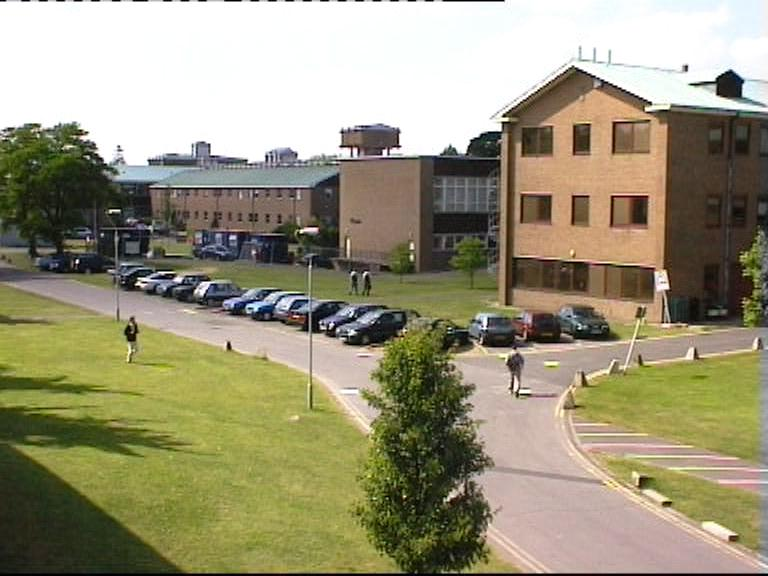
\includegraphics[width=1\linewidth]{figures/PETS2_highv.jpg}
  \caption{}
\end{subfigure}
\hfill
\begin{subfigure}{.48\linewidth}
  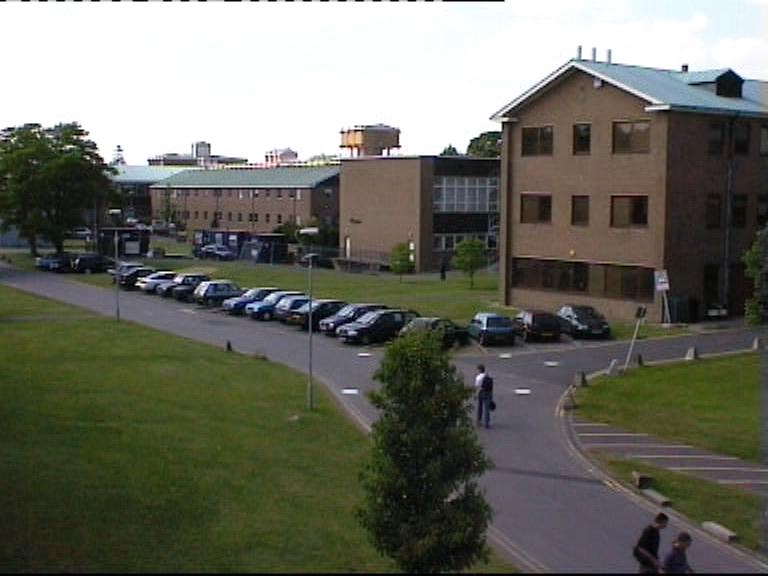
\includegraphics[width=1\linewidth]{figures/PETS2_lowv.jpg}
  \caption{}
\end{subfigure}
\caption{PETS2 experiencing both high illumination (a) and low illumination (b) (due to cloud cover).}
\label{fig:pets2illum}
\end{figure}

\begin{figure}
\centering
\begin{subfigure}{.3\linewidth}
  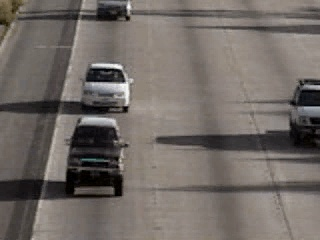
\includegraphics[width=1\linewidth]{figures/highway1_0045.jpg}
\end{subfigure}
\hfill
\begin{subfigure}{.3\linewidth}
  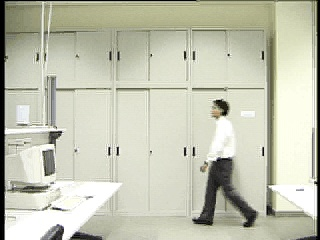
\includegraphics[width=1\linewidth]{figures/lab_0151.jpg}
\end{subfigure}
\hfill
\begin{subfigure}{.3\linewidth}
  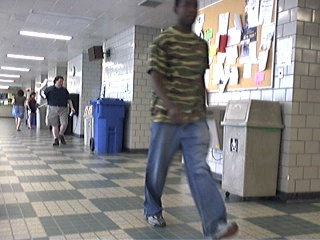
\includegraphics[width=1\linewidth]{figures/hallway_0164.jpg}
\end{subfigure}
\hfill
\begin{subfigure}{.3\linewidth}
  
\includegraphics[width=1\linewidth]{figures/highway1_gt_0045.jpg}
  \caption{}
\end{subfigure}
\hfill
\begin{subfigure}{.3\linewidth}
  
\includegraphics[width=1\linewidth]{figures/lab_gt_0151.jpg}
  \caption{}
\end{subfigure}
\hfill
\begin{subfigure}{.3\linewidth}
  
\includegraphics[width=1\linewidth]{figures/hallway_gt_0164.jpg}
  \caption{}
\end{subfigure}

\caption{Datasets collected for ATON: (a) aton\_highway1, (b) aton\_lab, and (c) aton\_hallway.}
\label{fig:datasetsgt}
\end{figure}

\FloatBarrier
\subsubsection{Assessment Tools}

The first stage of our methodology is an exploration of the sensitivity of shadow removal algorithms to environmental and parametric change. We developed tools to assist intuition regarding an algorithm's performance, capable of allowing a user to manually tune an algorithm parameter, and observe its effect on performance.

To better understand an algorithm's dependence on a parameter, a framework was required to rapidly modify the parameter in question. The initial implementation of the shadow removal methods, courtesy of Sanin et al. \cite{shadowssourceforge}, contained relevant parameters hard-coded into the algorithms. Each algorithm therefore required re-compilation to bring any modifications to fruition. This shortcoming was rectified by extracting each parameter and organizing them into an \textit{.ini} file. By utilizing username \textit{brofield}'s SimpleINI architecture, hosted on Github \cite{simpleini}, parameters can be either set extemporaneously or altered by an external script. An example SimpleIni .ini file is shown in Figure \ref{fig:simpleini}.

\begin{figure}
  \centering
  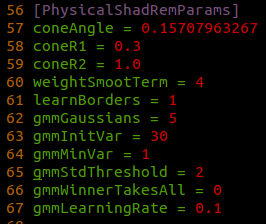
\includegraphics[width=.5\linewidth]{figures/simpleini.png}
  \caption{An example SimpleINI file. Parameters taken from this file are used to adjust values in real-time.}
  \label{fig:simpleini}
\end{figure}

Graphical tools (GUI) were then developed to rapidly assess and visualize a parameter's affect on shadow removal. Each shadow removal method was modified to accept arbitrary parameter values in real-time from the .ini file. These parameters were then tied to graphical sliders (from OpenCV's highgui library \cite{opencv}) dictating their range and value. Any numerical parameter that has the potential to modify the Detection or Discrimination rates of a shadow removal method is included in the GUI. An example of the GUI is seen in Figure \ref{fig:guitools}. The process in which the GUI modifies and displays parameters is illustrated in Figure \ref{fig:guimodel}.

\begin{figure}
  \centering
  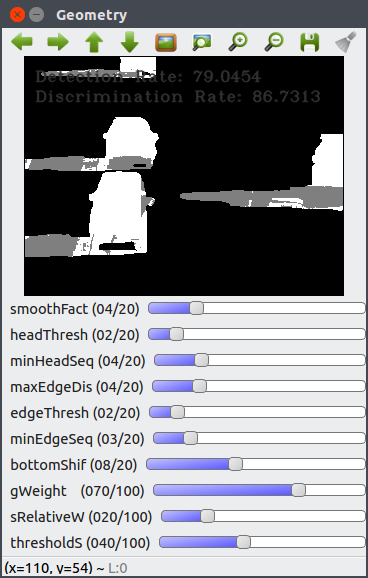
\includegraphics[width=.45\linewidth]{figures/geo_highway1_default.png}

\caption{GUI tools created using OpenCV, displaying Geometry shadow removal.}
\label{fig:guitools}
\end{figure}

\begin{figure}
  \centering
  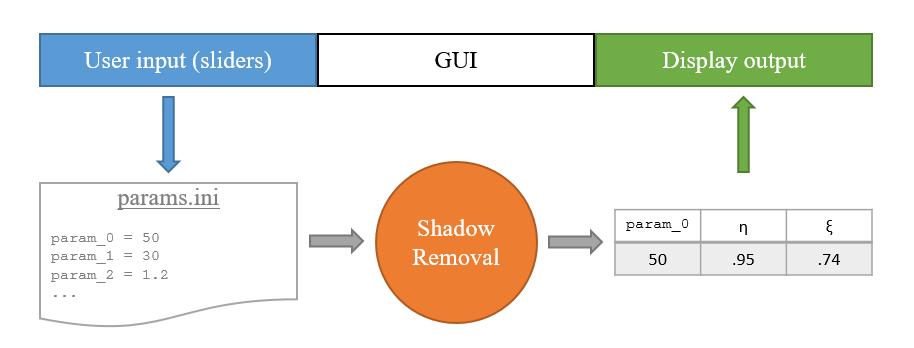
\includegraphics[width=1\linewidth]{figures/gui_model.png}
  \caption{The GUI takes user input through sliders, updates values in a .ini file, which are used to produce a new output image indicating shadow versus foreground pixels with the corresponding detection and discrimination rates. The GUI then visualizes this output.}
  \label{fig:guimodel}
\end{figure}

The display is updated in real-time with both a visual representation of detected shadow pixels (in gray), and a quantified display of both the exact detection and discrimination rates, computed based on the ground truth. Leveraging human perception, the graphical tools enabled rapid evaluation of the sensitivity of an algorithm to changes in parameter values within specific scenes.

\FloatBarrier
%%%
\subsubsection{Determining Optimal Parameter Values}
%%%

Modifying the algorithms to accept arbitrary parameter value settings at each frame enables us to create batch jobs to systematically vary parameter values across multiple runs. This allows us to meticulously sweep a given parameter ($pr$) through a specified range and record its corresponding affect upon detection and discrimination rates. Figure \ref{fig:guiiterate} illustrates the data collection process. The calculated detection and discrimination responses to change in $pr$ are recorded as the functions $\eta(pr)$ and $\xi(pr)$, respectively. Both $\eta(pr)$ and $\xi(pr)$ are determined for one frame. Figure \ref{fig:campusddscore}(a) demonstrates an example of these responses.

\begin{figure}
  \centering
  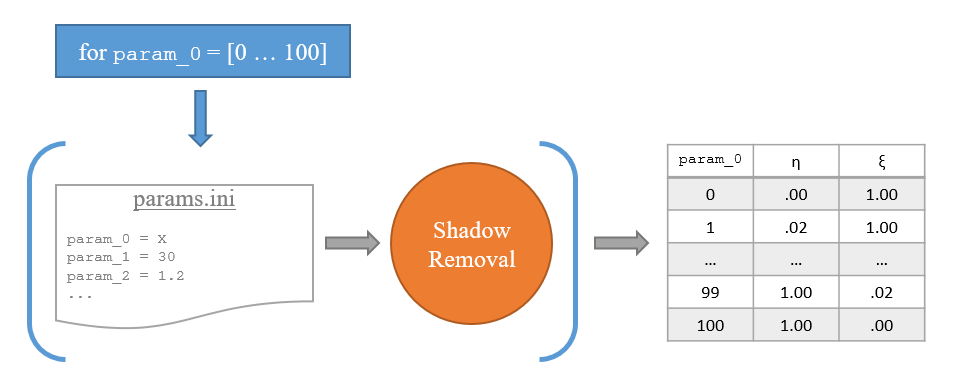
\includegraphics[width=1\linewidth]{figures/gui_iterate.png}
  \caption{For one frame, a parameter is systematically iterated to provide detection/discrimination results for each possible parameter value.}
  \label{fig:guiiterate}
\end{figure}

\begin{figure}
  \centering
  \begin{subfigure}{.8\linewidth}
  	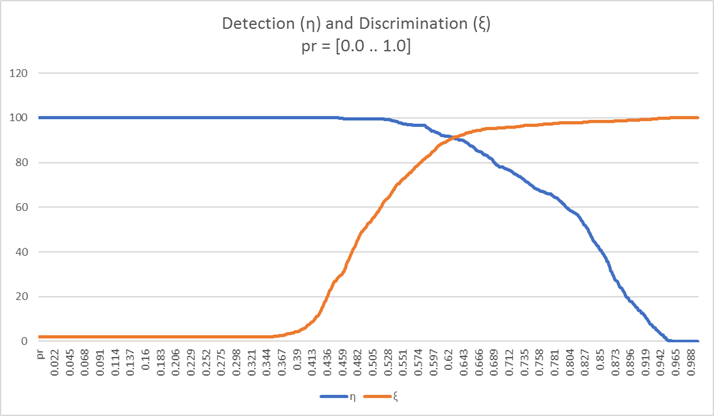
\includegraphics[width=1\linewidth]{figures/campus_dd.jpg}
  \caption{}
  \end{subfigure}
  \hfill
  \begin{subfigure}{.8\linewidth}
  	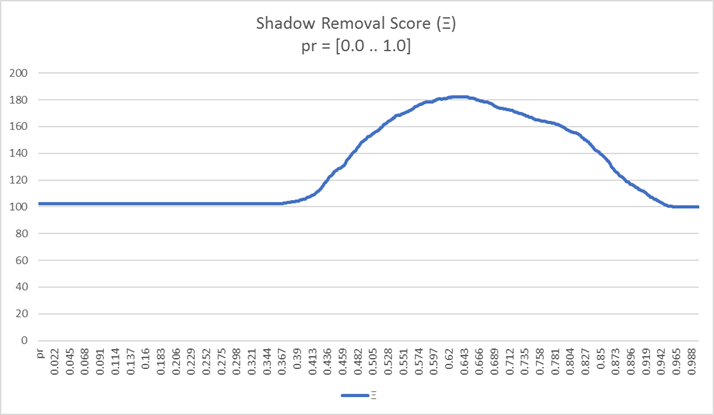
\includegraphics[width=1\linewidth]{figures/campus_score.jpg}
  \caption{}
  \end{subfigure}
\caption{(a) Detection (blue) and Discrimination (orange) rates are charted against the iterated parameter value $pr$ (x-axis). For each parameter value, detection and discrimination are summed to produce a removal efficacy score $\Xi(pr)$. The global maximum of this value is the optimal parameter value ($pr$*).}
\label{fig:campusddscore}
\end{figure}

We also utilize the iterative process to determine the optimal value of $pr$ for each frame in a dataset, i.e., which $pr$ value yields the greatest improvements in detection and discrimination. This optimal value is denoted as $pr$*. The detection and discrimination rates are summed, resulting in a shadow removal score $\Xi(pr)$ (Eqn. \ref{eqn:score}), which quantifies the efficacy of the shadow removal algorithm given a certain $pr$ value. Figure \ref{fig:campusddscore}(b) illustrates the score calculated using the responses found in Figure \ref{fig:campusddscore}(a). We define the optimal value $pr$* as the global maximum of $\Xi(pr)$ (Eqn. \ref{eqn:optscore}).

\begin{equation}
\Xi(pr) = \eta(pr) + \xi(pr)
\label{eqn:score}
\end{equation}

\begin{equation}
pr\emph{*} = max(\Xi(pr))
\label{eqn:optscore}
\end{equation}

To assess the performance of algorithms throughout a dataset, $pr$* is calculated for each frame. The $pr$* values are used to determine degrees of correlation for an environment, and set the foundation for a general model of arbitrary shadow removal improvement.

\FloatBarrier
\subsection{Algorithm Selection Strategy} \label{section:selectalgorithm}

Using the tools detailed in section \ref{section:datacollection}, we perform a brief qualitative assessment of the shadow removal algorithms' sensitivity. Given the diversity of shadow removal methods, a wide array of environmental factors may potentially influence an even wider array of algorithmic parameters. The scope of this research has therefore been focused on identifying a suitable algorithm to assess, linking a parameter (intrinsic to this algorithm) to unique environmental properties or changes, and developing a model for real-time parameter adaptation based on correlations found.
%and begin the construction of a general model of shadow removal improvement given analogous parameters.

%Identifying an appropriate algorithm for assessment means highlighting a shadow removal method that demonstrates consistently reasonable sensitivity to changes in environmental characteristics. Simultaneously, a candidate for deeper analysis must demonstrate consistency in its detection/discrimination integrity throughout most frames of a dataset, with few sizable deviations. If the study were not constrained in this manner, the motivation of this research quickly becomes redundant, as the sheer amount of interdependent variables brings the problem to levels generally reserved for unsupervised clustering and other big-data approaches. As this study means to link qualitative environmental characteristics to quantitative tangible improvement, this approach would detour research into a different realm entirely.

Candidate shadow removal algorithms are evaluated according to the correlation between their efficacy (in terms of detection and discrimination rates) over time, and qualitative observations attributed to a dataset; e.g., the PETS1 dataset experiences a large illumination change midway through its sampling, which is taken into account when searching for trends among the accuracy of a candidate method. Figure \ref{fig:selectinganalgorithm} demonstrates shadow detection rates using the PETS1 dataset, for each shadow removal algorithm.

\begin{sidewaysfigure}
\centering
\caption{Shadow detection ($\eta$)(orange) for each algorithm, run on the PETS1 dataset during an illumination change. Overall brightness of a scene is shown in gray.}
\begin{subfigure}{.32\linewidth}
  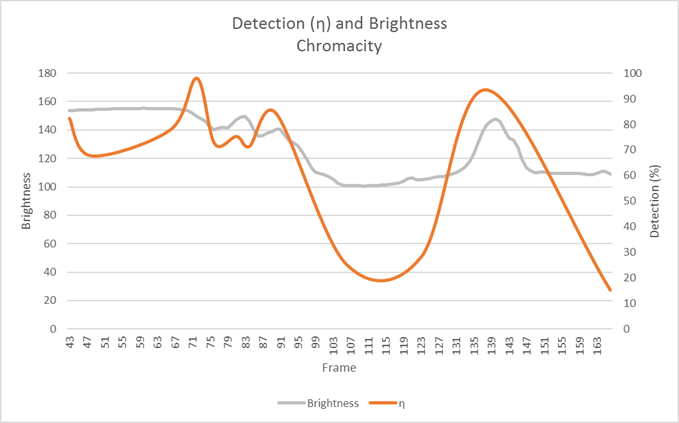
\includegraphics[width=1\linewidth]{figures/selectinganalgorithm_chromacity.jpg}
  \caption{Chromacity removal.}
\end{subfigure}
\hfill
\begin{subfigure}{.32\linewidth}
  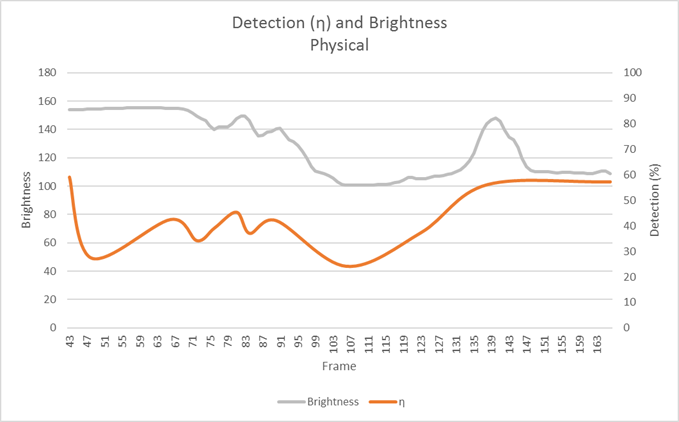
\includegraphics[width=1\linewidth]{figures/selectinganalgorithm_physical.jpg}
  \caption{Physical removal.}
\end{subfigure}
\hfill
\begin{subfigure}{.32\linewidth}
  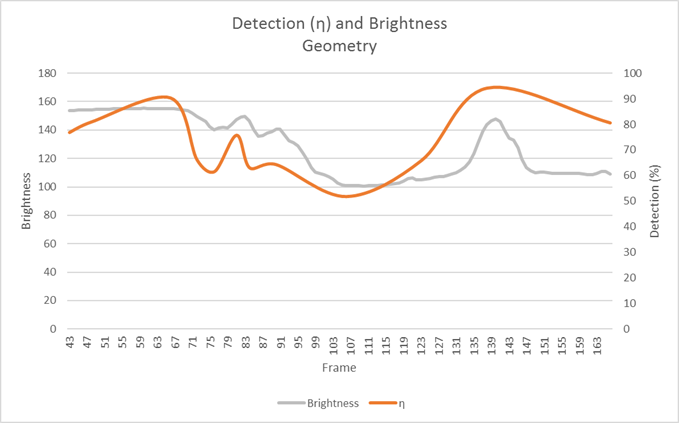
\includegraphics[width=1\linewidth]{figures/selectinganalgorithm_geometry.jpg}
  \caption{Geometry removal.}
\end{subfigure}
\hfill
\begin{subfigure}{.32\linewidth}
  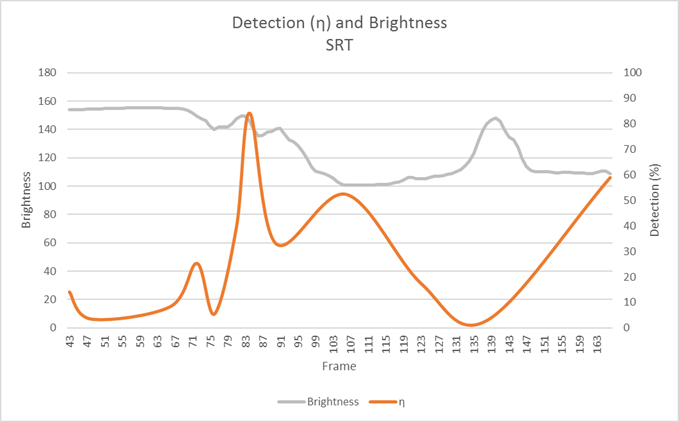
\includegraphics[width=1\linewidth]{figures/selectinganalgorithm_srt.jpg}
  \caption{Small-Region Texture removal.}
\end{subfigure}
%\hfill
\begin{subfigure}{.32\linewidth}
  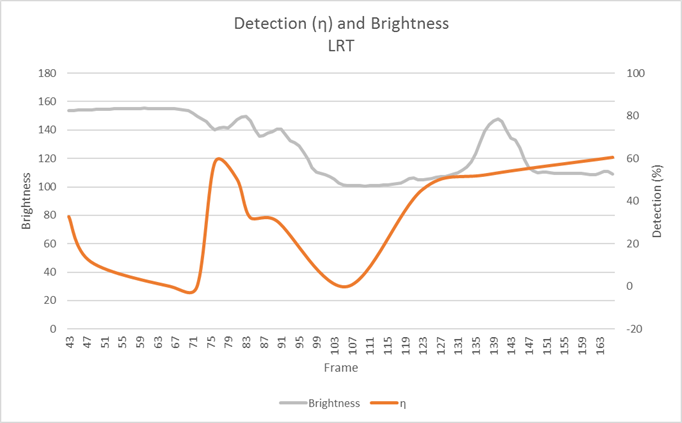
\includegraphics[width=1\linewidth]{figures/selectinganalgorithm_lrt.jpg}
  \caption{Large-Region Texture removal.}
\end{subfigure}
\label{fig:selectinganalgorithm}
\end{sidewaysfigure}

\FloatBarrier
\subsubsection{Evaluation of Methods}

We evaluate popular shadow removal methods introduced in section \ref{section:removalmethods}: Chromacity, Physical, Geometry, SRT, and LRT. This section describes our rationale for using Physical shadow removal as part of our proof-of-concept, implemented starting in section \ref{section:selectparameter}. Our evaluation considers the tunable parameters of an algorithm, dependence on environmental properties and content, and sensitivity of relevant parameters.

A parameter's sensitivity is evaluated by viewing its detection and discrimination responses ($\eta(pr)$, $\xi(pr)$). Figure \ref{fig:paramsensitivity} illustrates what is considered a sensitive parameter. A parameter is considered sensitive when a narrow range of parameter values affect detection and discrimination rates disproportionately. This sensitivity causes problems for an adaptive model, as the range of potential optimal parameter values ($pr$*) is too small to correlate with environmental properties. 

\begin{figure}
\centering
\begin{subfigure}{.49\linewidth}
  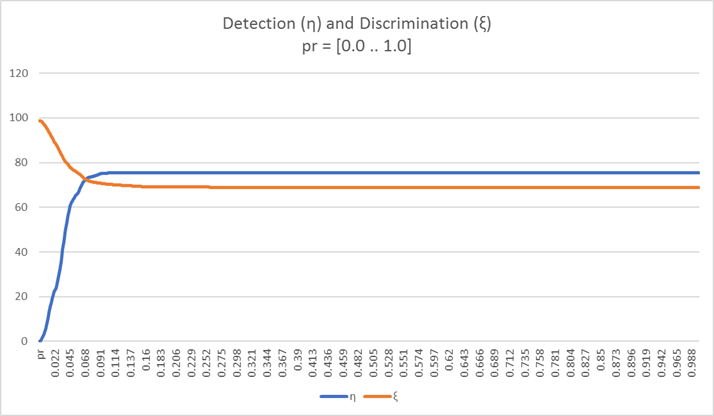
\includegraphics[width=1\linewidth]{figures/sensitive_param.jpg}
  \caption{}
\end{subfigure}
\hfill
\begin{subfigure}{.49\linewidth}
  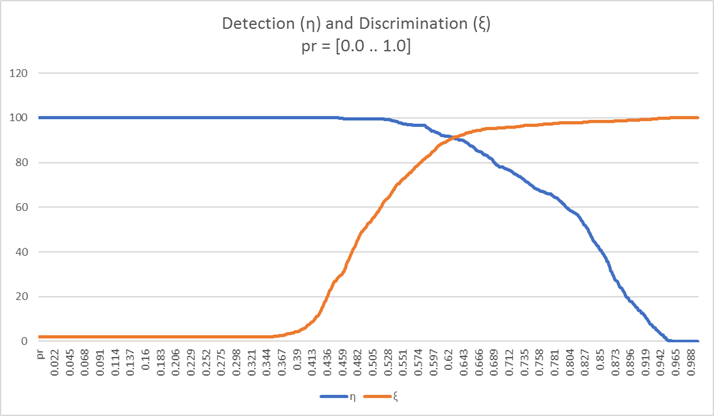
\includegraphics[width=1\linewidth]{figures/campus_dd.jpg}
  \caption{}
\end{subfigure}

\caption{(a) depicts a sensitive parameter, while (b) represents a typical parameter.}
\label{fig:paramsensitivity}
\end{figure}

%Both Geometry removal and SRT removal were shown to behave highly erratically from frame to frame even within an environmentally consistent dataset. Geometry-based removal remains dependent on the shape and consistency of processed foreground objects, and therefore dependent on the consistency of whichever foreground extractor is used for a scene. This dependency is not related to the properties of shadows within an environment, therefore we do not pursue further analysis with Geometry removal. SRT removal is based upon a series of Gabor filters used to characterize textural patches found in shadows, and match them to a corresponding background model. This technique requires that shadows cover textural portions of the background model large enough to perform meaningful analysis. The algorithm carries with it no meaningful contingencies for this limitation. The parameters associated with SRT removal define little avenue for improvement of shadow removal in most cases, and defines no avenue for cases mentioned where the shadows are too small. This dependence on a shadow's area, coupled with no parameters suitable to improve detection, eliminated SRT removal from candidacy. 

Both Geometry removal and SRT removal were shown to behave highly erratically from frame to frame even within an environmentally consistent dataset, demonstrated in Figure \ref{fig:geosrterratic}. Geometry-based removal remains dependent on the shape and consistency of processed foreground objects, and therefore dependent on the consistency of whichever foreground extractor is used for a scene. Furthermore, the algorithmic parameters associated with Geometry removal apply only to scenes in which the previous dependency is already fulfilled, i.e., the tunable parameters are relevant only to the geometric shapes necessary to enable Geometry removal. These dependencies are not related to the properties of shadows within an environment, therefore we do not pursue further analysis with Geometry removal. SRT removal is based upon a series of Gabor filters used to characterize textural patches found in shadows, and match them to a corresponding background model. This technique requires that shadows cover textural portions of the background model large enough to perform meaningful analysis. Manual tuning of SRT's algorithmic parameters provides no benefit to the algorithms detection or discrimination rates. This dependence on a shadow's area, coupled with the lack of parameters suitable to improve shadow removal, eliminated SRT removal from candidacy. 

\begin{figure}
\centering
\begin{subfigure}{.8\linewidth}
  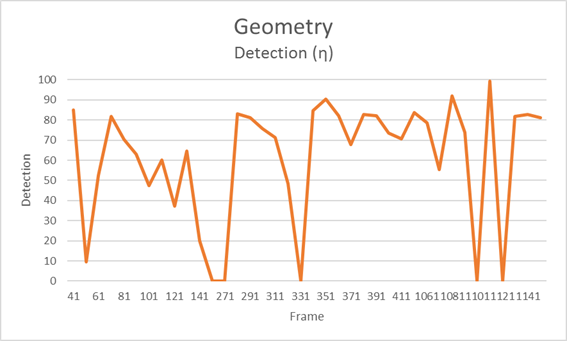
\includegraphics[width=1\linewidth]{figures/campus_geo_erratic.jpg}
  \caption{Geometry}
\end{subfigure}
\hfill
\begin{subfigure}{.8\linewidth}
  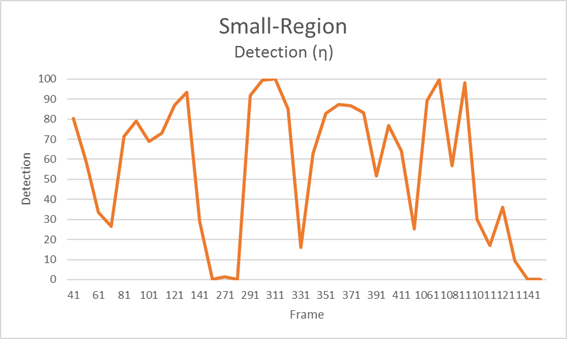
\includegraphics[width=1\linewidth]{figures/campus_srt_erratic.jpg}
  \caption{Small-Region Texture}
\end{subfigure}

\caption{(a) and (b) showcase erratic shadow detection run on the dataset aton\_campus, which experiences no significant illumination change.}
\label{fig:geosrterratic}
\end{figure}

%Sanin et al.'s Large-Region Texture algorithm was also eliminated from the assessment due to its temperamental inter-frame performance, similar to the methods above. Some environments, such as the roadways of aton\_highway3, yielded null detections for all frames \textbf{NOTE: This specific test needs to be rerun, I know why the NULLs happened. Everything else is fine though}. The Large-Region Texture algorithm recognizes the pitfalls of the Small-Region approach, such as overly-small texture regions, and attempts to correct them using hard-coded parameters. Unfortunately, the algorithm as a whole displays an overly large sensitivity to change, both inter and intra-dataset (see Figure \ref{fig:lrt_sensitivity}). In a larger scoped study, one may approach this algorithm as an ideal candidate for potential improvement, given its large swath of tunable parameters and variable responses. However, for those reasons it was excluded from the remainder of this study. By selecting an algorithm with more controlled responses to change of environment, we can extend insights gleaned into improvements for other algorithms, including this one.

Sanin et al.'s Large-Region Texture algorithm was also eliminated from the assessment due to its inconsistent shadow removal, similar to Geometry and SRT removal (Figure \ref{fig:lrt_sensitivity}). Some environments, such as the roadways of aton\_highway1, yielded null detections for all frames. The Large-Region Texture algorithm recognizes the pitfalls of the Small-Region approach, such as restrictive texture regions, and attempts to correct them using hard-coded parameters. The algorithm primarily displays a sensitivity to environment, as identical parameter values produce vastly disparate shadow removal performances (Figure \ref{fig:lrt_sensitivity}). 

\begin{figure}
\centering
\begin{subfigure}{.8\linewidth}
  \centering
  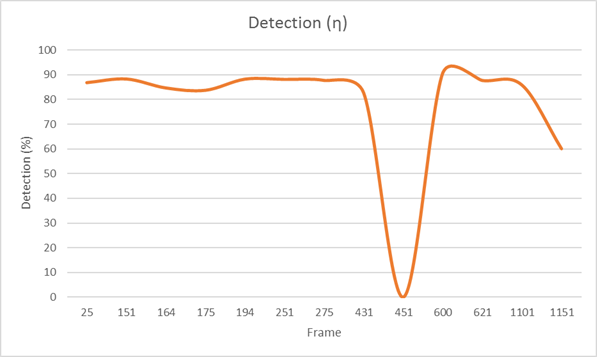
\includegraphics[width=1\linewidth]{figures/lrt_sensitivity_2.jpg}
  \caption{}
\end{subfigure}
\hfill
\begin{subfigure}{.8\linewidth}
  \centering
  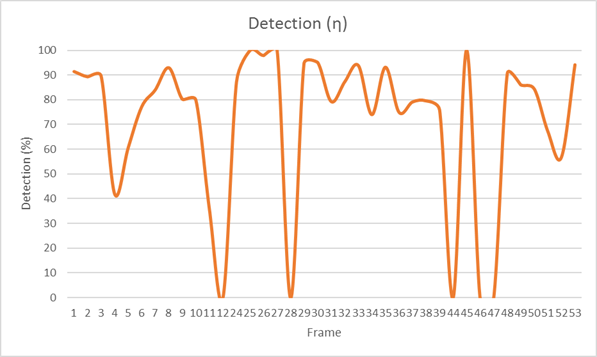
\includegraphics[width=1\linewidth]{figures/lrt_sensitivity_1.jpg}
  \caption{}
\end{subfigure}
\caption{(a) Run on aton\_hallway, LRT shows consistent shadow removal accuracy, with occasional dips. (b) Run on aton\_campus, LRT performs erratically.}
\label{fig:lrt_sensitivity}
\end{figure}

LRT also demonstrates varying levels of parametric sensitivity, also dependent on the deployment environment. For example, the parameter \textit{avgAttenThresh} is highly sensitive, shown in Figure \ref{fig:avgattenthresh_response}, and has only one value per frame that affects detection and discrimination. Furthermore, shadow removal is affected disproportionately to \textit{avgAttenThresh}, with shadow detection rates often dropping to zero when affected. LRT has several parameters that behave in similar ways, demonstrating a lack of scalability for changing environmental properties.

\begin{figure}
  \centering
  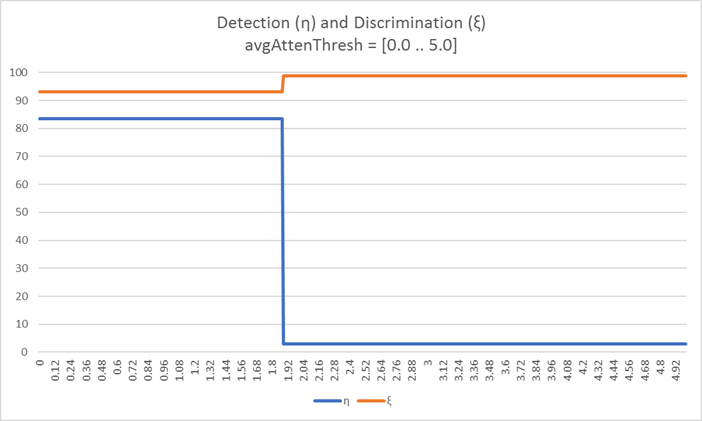
\includegraphics[width=.8\linewidth]{figures/highway1_avgAttenThresh_response.jpg}

\caption{The LRT parameter \textit{avgAttenThresh} is highly sensitive, demonstrating a narrow range for which LRT removal accuracy is affected. LRT's removal accuracy response is shown, using the aton\_highway1 dataset.}
\label{fig:avgattenthresh_response}
\end{figure}

%Finally, both Chromacity-based and Physical-based shadow removal held the qualities ascribed to a suitable algorithm for exploration. In both cases, trends are observed, consistency of detection is within reasonable range, and the modification of parameters produces a scalable and easily observable response. This is visualized in Figure \ref{fig:similarities}.

\begin{figure}
\centering
  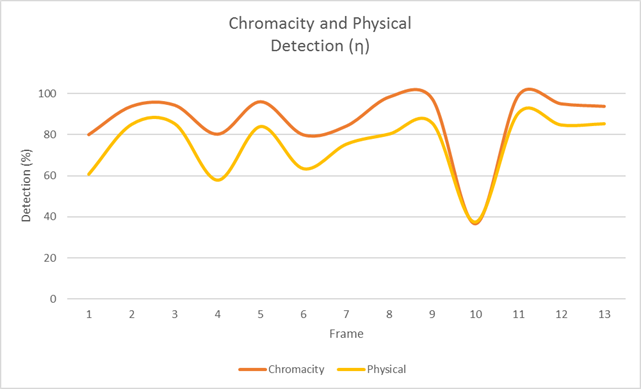
\includegraphics[width=.8\linewidth]{figures/similarities_chromacity_physical_hallway.jpg}

\caption{Chromacity and Physical shadow removal demonstrate similar shadow detection results run on aton\_hallway.}
\label{fig:similarities}
\end{figure}

Chromacity and Physical shadow removal provide tunable parameters that lie within acceptable ranges of sensitivity. An example of an acceptable range of sensitivity is seen in Figure \ref{fig:paramsensitivity}(b). The shadow removal algorithms often respond similarly to the diversity of environments in this study; for example, Figure \ref{fig:similarities} illustrates comparable detection rates for the aton\_hallway dataset. Chromacity and Physical shadow removal also display consistency between datasets, i.e., none of the datasets provide particularly poor results that are not linked to an environmental property change, such as illumination change. The Chromacity removal algorithm succeeds due to the tendency of shadows (within a dataset) to remain a consistent darkness when compared to the corresponding background model. However, this simple approach can prove problematic when illumination changes occur within a dataset. Physical shadow removal utilizes a similar system of gauging a shadow's darkness compared to a background model - what is referred to as a weak detector \cite{cucchiara2003detecting, sanin2010improved, huang2009moving} - and implicitly suffers similar breakdowns of detection when presented with significant illumination flux within a dataset. Although they both suffer, Physical shadow removal employs a strong detector to increase detection and discrimination at the cost of processing time. In the end, Physical shadow removal was selected as the main experimental framework for this study, in part due to Physical shadow removal's more sophisticated model.

\FloatBarrier
\subsection{Selecting a Parameter of Physical Shadow Removal} \label{section:selectparameter}

Physical shadow removal operates in two stages: the weak detector, and the strong detector. The weak detector typically identifies candidate shadow pixels simply by eliminating impossible pixels, i.e., pixels that are brighter than the background model. The remaining foreground pixels are then provided as candidate pixels to the strong detector, which characterizes these pixels as either shadow or foreground. Our assessment of algorithmic parameters explores parameters in both of these detector spaces. Before we can illustrate which parameters were considered for experimentation, we must first understand each parameter's place within the algorithm.

\subsubsection{Weak Detector - Physical Shadow Removal}

The purpose of the weak detector is to prevent impossible pixels from being fed to the strong detector. The weak detector in Physical shadow removal functions similarly to the Chromacity shadow removal process; the candidate pixel is evaluated by its distance from a corresponding background pixel and sorted accordingly. The weak detector is visually, and technically, a cone projected in an RGB plane indicating the range in which a normalized shadow pixel may lie with respect to a background model. Normalizing the shadow pixel's position relative to the background model is accomplished by computing the angular distance between the RGB vector of the foreground and the RGB vector of the background. The resultant represents the color-space deviation from foreground to background. This threshold parameter is named \textit{coneAngle} within the Physical shadow removal algorithm. The cone represents two dimensions: color deviation ($\theta$), and intensity (or brightness) deviation. A foreground pixel is considered a possible shadow if the normalized ratio of foreground to background brightness (scaled by a function of the color deviation ($cos(\theta)$), is within a pre-defined brightness range. The tolerable brightness range, delimited by parameters named \textit{coneR1} (minimum) and \textit{coneR2} (maximum), is hard-coded within the original algorithm to be 0.3 to 1.0. 
%\cite{huang2009moving} illustrates the conic model in Figure \ref{fig:cone_physical}.

%\begin{figure}
%  \centering
%  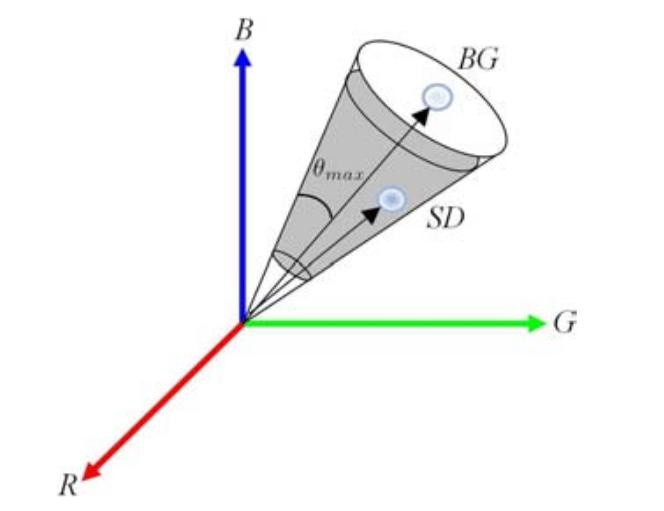
\includegraphics[width=.8\linewidth]{figures/cone_physical.jpg}
%  \caption{The conical volume describing the tolerable brightness range of a shadow pixel (\textit{SD}), in relation to a its illuminated background pixel (\textit{BG}). The maximal allowable color deviation, $\theta_{max}$, is represented in the algorithm as \textit{coneAngle}. Figure from \cite{huang2009moving}.}
%  \label{fig:cone_physical}
%\end{figure}

The main components of the weak detector are parameterized within the algorithm to fit a general model; \textit{coneR1} $<$ $x$ $<$ \textit{coneR2} as an intensity range works reasonably well for many scenes, but there exists an optimal range for any given environment. Similarly, the optimal color angle ($\theta$) between foreground and background vectors is dependent on environmental parameters. These parameters, \textit{coneR1}, \textit{coneR2}, and \textit{coneAngle} are therefore considered when looking for correlations with environmental conditions.

\FloatBarrier
\subsubsection{Strong Detector - Physical Shadow Removal}

After the weak detector removes impossible candidates for shadow pixels, a Gaussian Mixture Model (GMM) is used to learn the color features of shadow pixels when compared to background pixels. Using the remaining pixels, the GMM estimates the normalized spectral ratio for shadows in a scene, i.e., the ratio of spectral illuminants \cite{huang2009moving, sato2015foreground, lee2017shadow}. More information on spectral illuminants can be found in section \ref{section:nonlinearatten}. The GMM is a framework based upon Expectation Maximization and learning over time; therefore, the initial parameters presented in the algorithm have little influence over the efficacy of shadow removal. Shadow removal displayed sensitivity to only one significant parameter, \textit{postThresh}, the parameter controlling the posterior threshold. The posterior threshold is the threshold governing shadow/foreground assignment after the posterior probability of a pixel is determined via the GMM. Since the GMM adapts to its environment, modifying the posterior threshold invalidates any learning the GMM has achieved. Therefore, correlating \textit{postThresh} to environmental properties is not performed in this study.

\subsubsection{Evaluation of Parameters}

Due to their integral nature to both the weak and strong detectors, the parameters \textit{coneR1} and \textit{coneAngle} are evaluated for their effect on shadow removal. Each parameter is shown to have a pronounced effect on shadow removal. 

\begin{figure}
  \begin{subfigure}{.45\linewidth}
  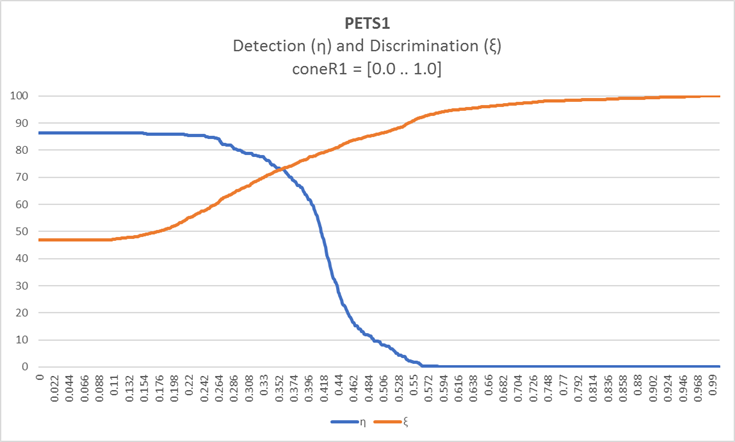
\includegraphics[width=1\linewidth]{figures/pets1_coneR1_response.jpg}
  \caption{PETS1}
\end{subfigure}
\hfill
\begin{subfigure}{.45\linewidth}
  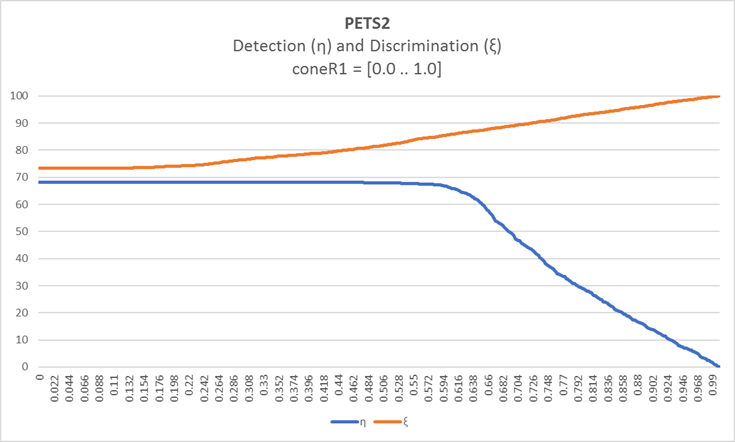
\includegraphics[width=1\linewidth]{figures/pets2_coneR1_response.jpg}
  \caption{PETS2}
\end{subfigure}
\hfill
\begin{subfigure}{.45\linewidth}
  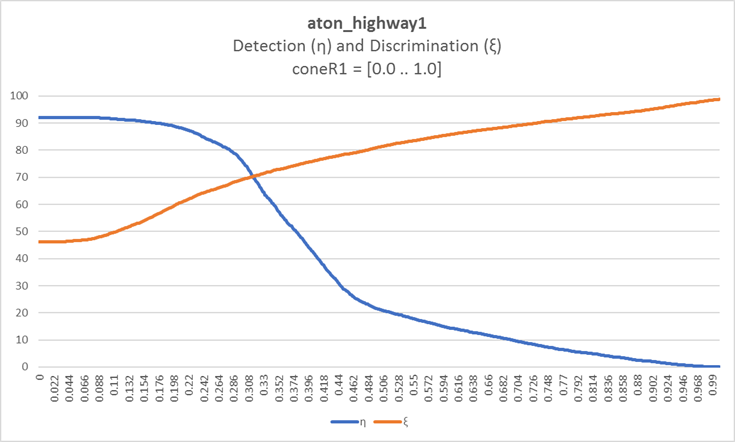
\includegraphics[width=1\linewidth]{figures/highway1_coneR1_response.jpg}
  \caption{aton\_highway1}
\end{subfigure}
\hfill
\begin{subfigure}{.45\linewidth}
  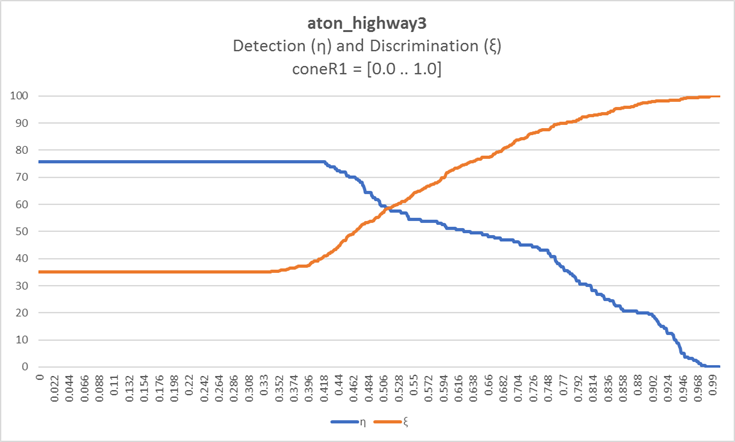
\includegraphics[width=1\linewidth]{figures/highway3_coneR1_response.jpg}
  \caption{aton\_highway3}
\end{subfigure}
\hfill
\begin{subfigure}{.45\linewidth}
  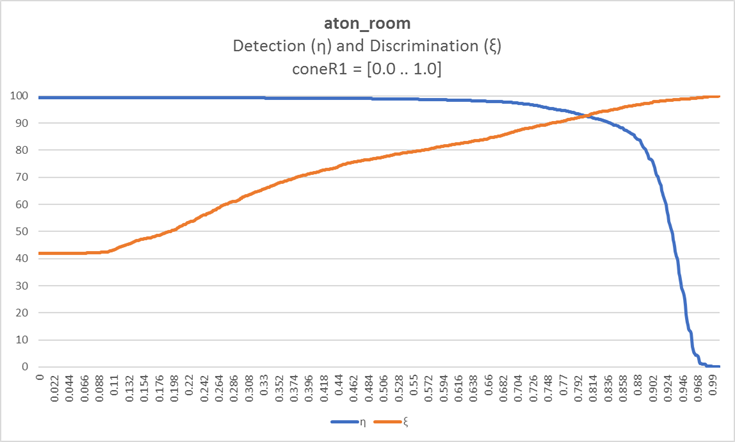
\includegraphics[width=1\linewidth]{figures/room_coneR1_response.jpg}
  \caption{aton\_room}
\end{subfigure}
\hfill
\begin{subfigure}{.45\linewidth}
  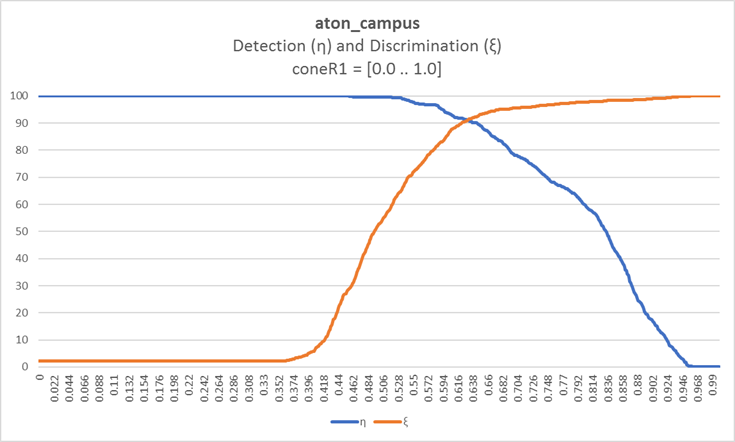
\includegraphics[width=1\linewidth]{figures/campus_coneR1_response.jpg}
  \caption{aton\_campus}
\end{subfigure}
\hfill
\begin{subfigure}{.45\linewidth}
  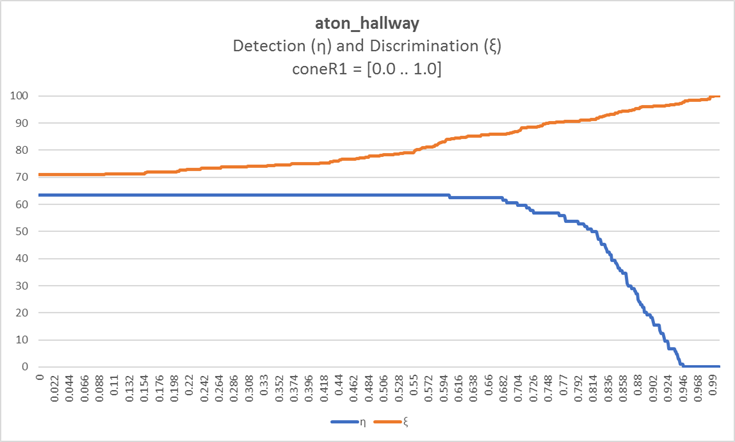
\includegraphics[width=1\linewidth]{figures/hallway_coneR1_response.jpg}
  \caption{aton\_hallway}
\end{subfigure}
\hfill
\begin{subfigure}{.45\linewidth}
  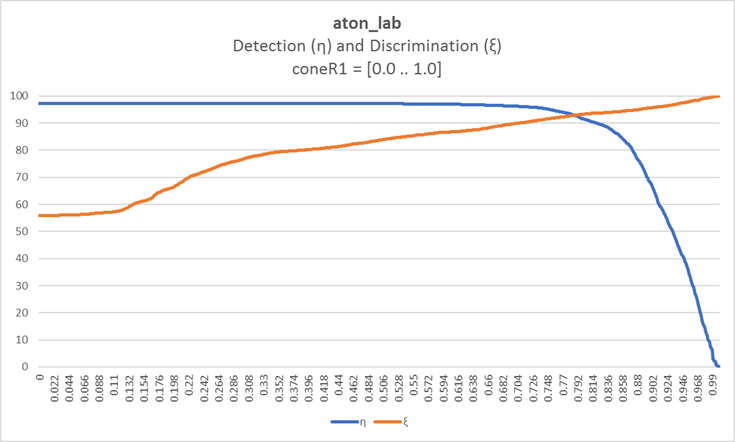
\includegraphics[width=1\linewidth]{figures/lab_coneR1_response.jpg}
  \caption{aton\_lab}
\end{subfigure}

\caption{Detection (blue) and discrimination (orange) rates are calculated as the value of \textit{coneR1} is varied from [0.0 .. 1.0]. Full results found in appendices.}
\label{fig:coneR1_iterate}
\end{figure}

\begin{figure}
  \begin{subfigure}{.45\linewidth}
  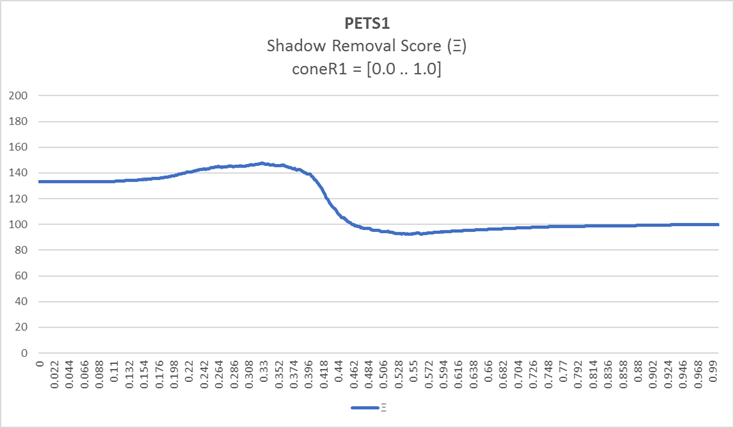
\includegraphics[width=1\linewidth]{figures/pets1_coneR1_score.jpg}
  \caption{PETS1}
\end{subfigure}
\hfill
\begin{subfigure}{.45\linewidth}
  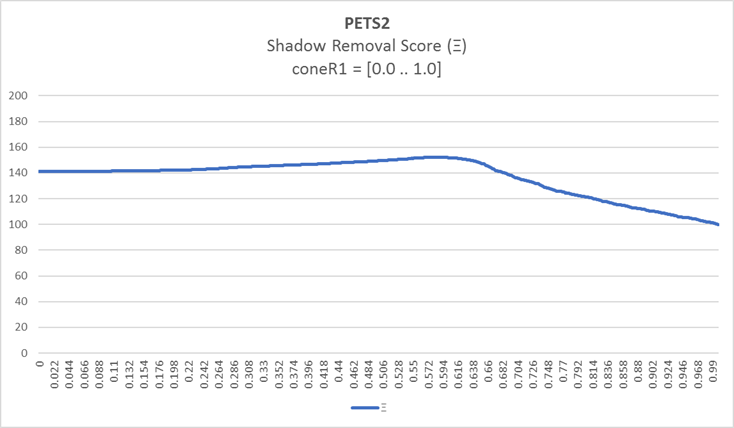
\includegraphics[width=1\linewidth]{figures/pets2_coneR1_score.jpg}
  \caption{PETS2}
\end{subfigure}
\hfill
\begin{subfigure}{.45\linewidth}
  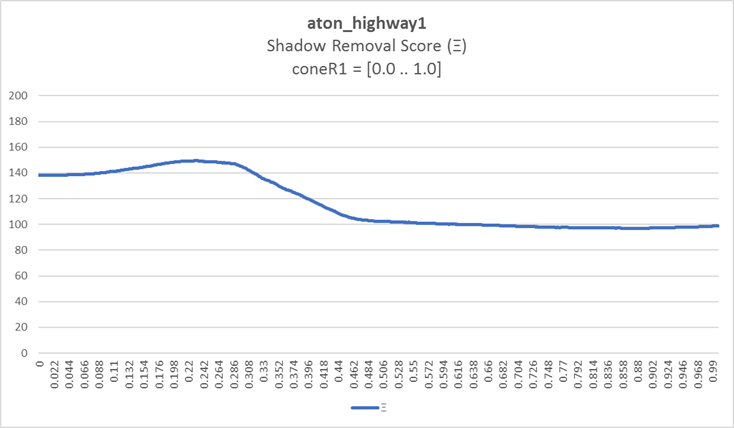
\includegraphics[width=1\linewidth]{figures/highway1_coneR1_score.jpg}
  \caption{aton\_highway1}
\end{subfigure}
\hfill
\begin{subfigure}{.45\linewidth}
  \includegraphics[width=1\linewidth]{figures/highway3_coneR1_score.jpg}
  \caption{aton\_highway3}
\end{subfigure}
\hfill
\begin{subfigure}{.45\linewidth}
  \includegraphics[width=1\linewidth]{figures/room_coneR1_score.jpg}
  \caption{aton\_room}
\end{subfigure}
\hfill
\begin{subfigure}{.45\linewidth}
  \includegraphics[width=1\linewidth]{figures/campus_coneR1_score.jpg}
  \caption{aton\_campus}
\end{subfigure}
\hfill
\begin{subfigure}{.45\linewidth}
  \includegraphics[width=1\linewidth]{figures/hallway_coneR1_score.jpg}
  \caption{aton\_hallway}
\end{subfigure}
\hfill
\begin{subfigure}{.45\linewidth}
  \includegraphics[width=1\linewidth]{figures/lab_coneR1_score.jpg}
  \caption{aton\_lab}
\end{subfigure}

\caption{Example score ($\Xi$) of a frame for each dataset. Full results found in appendices.}
\label{fig:coneR1_iterate_score}
\end{figure}

Figure \ref{fig:coneR1_iterate} demonstrates \textit{coneR1}'s contribution to detection/discrimination across datasets. \textit{coneR1}'s effect on shadow removal remains consistent and scalable. The parameter is exercised through a large range, with an equally large range of resultant detection and discrimination rates. Figure \ref{fig:coneR1_iterate_score} shows that each dataset demonstrates an unambiguous maximum score, \textit{coneR1}*. The wider range and relatively coarse-grained nature of the parameter facilitates identifying trends and correlations with the iterations.

\FloatBarrier
\textit{coneR2} represents the upper limit of the cone describing a shadow pixel's color representation. While it serves a similar function as \textit{coneR1}, upon sensitivity testing, \textit{coneR2} was never found to contribute to higher detection and discrimination rates. Its default value (1.0) is also its optimal value (\textit{coneR2}*). Figure \ref{fig:coneR2_iterate} shows that the maximum of $\Xi$\textit{(coneR2)}, \textit{coneR2}*, is 1.0 across multiple datasets.

\begin{figure}
  \begin{subfigure}{.45\linewidth}
  \includegraphics[width=1\linewidth]{figures/campus_coneR2_response.jpg}
  \caption{aton\_campus ($\eta$, $\xi$)}
\end{subfigure}
\hfill
\begin{subfigure}{.45\linewidth}
  \includegraphics[width=1\linewidth]{figures/campus_coneR2_score.jpg}
  \caption{aton\_campus ($\Xi$)}
\end{subfigure}
\hfill
\begin{subfigure}{.45\linewidth}
  \includegraphics[width=1\linewidth]{figures/highway1_coneR2_response.jpg}
  \caption{aton\_highway1 ($\eta$, $\xi$)}
\end{subfigure}
\hfill
  \begin{subfigure}{.45\linewidth}
  \includegraphics[width=1\linewidth]{figures/highway1_coneR2_score.jpg}
  \caption{aton\_highway1 ($\Xi$)}
\end{subfigure}
\hfill
\begin{subfigure}{.45\linewidth}
  \includegraphics[width=1\linewidth]{figures/room_coneR2_response.jpg}
  \caption{aton\_room ($\eta$, $\xi$)}
\end{subfigure}
\hfill
\begin{subfigure}{.45\linewidth}
  \includegraphics[width=1\linewidth]{figures/room_coneR2_score.jpg}
  \caption{aton\_room ($\Xi$)}
\end{subfigure}

\caption{Parameter value responses for \textit{coneR2} for three datasets (aton\_campus, aton\_highway1, and aton\_room). Full results found in appendices.}
\label{fig:coneR2_iterate}
\end{figure}

\textit{coneAngle} inhabits too narrow a range of sensitivity to properly exploit (see results included in the appendices). Figure \ref{fig:coneAngle_iterate} illustrates the sensitivity of the parameter. Within the frames of a dataset, the calculated \textit{coneAngle}* values are within millionths of one another. Furthermore, \textit{coneAngle}* does not provide as large an improvement in shadow removal as \textit{coneR1}* does. The minimal removal improvement and narrow range of sensitive values makes further examination of \textit{coneAngle} difficult. For the duration of this study, environmental feature correlations were sought only in relation to \textit{coneR1}.

\begin{figure}
  \centering
  \begin{subfigure}{.8\linewidth}
  \includegraphics[width=1\linewidth]{figures/sensitive_param.jpg}
  \caption{}
\end{subfigure}
\hfill
\begin{subfigure}{.8\linewidth}
  \includegraphics[width=1\linewidth]{figures/sensitive_param_score.jpg}
  \caption{}
\end{subfigure}

\caption{(a) Shadow removal reponse (detection and discrimination) for \textit{coneAngle}, for aton\_highway1. (b) Shadow removal score for aton\_highway1. \textit{coneAngle}* is the maximum of the score.}
\label{fig:coneAngle_iterate}
\end{figure}

\FloatBarrier
\section{Assessment of Environmental Properties} \label{section:envassess}

We now create a proof-of-concept of our adaptive model, by correlating environmental properties with a previously assessed parameter \textit{coneR1}. We explore observed environmental properties within the datasets: attenuation and saturation. We also perform sensitivity analysis on multiple environmental properties (brightness functions, SIFT parameters) to explore their possible influence on correlation between \textit{coneR1}* and attenuation ($\alpha$). A model is given for using the observed environmental properties to calculate a new variable \textit{coneR1}$'$, which represents the adaptation of the \textit{coneR1} parameter to more closely match the curated \textit{coneR1}* ideal value.

\subsection{Previous Work - Large Region Texture Removal} \label{section:prevworkLRT}

Of all the leading shadow removal algorithms we evaluated, only one attempts to adapt its parameters to its current environment. In Sanin et al.'s LRT shadow removal \cite{sanin2010improved}, there are three examples of ambient environment properties taken into account: average saturation (of foreground pixels), average attenuation (from foreground to background), and average perimeter size of foreground objects. These three global properties govern the value of certain algorithm parameters.

LRT removal checks the average perimeter of foreground objects in a frame against a predetermined threshold. Average perimeter is linked to three additional algorithm parameters that control the size of the texture region being matched to identify shadows. If the average perimeter is above the predetermined threshold, the range of area for foreground/background correlation is expanded. The average perimeter is computed on a per-frame basis, while the threshold remains static.

LRT removal, like Physical shadow removal, uses a weak detector to retrieve candidate (shadow) pixels. The candidate shadow pixels must fit within a certain range of Hue (H), Saturation (S), and Value (V)(or Brightness) when compared against the background model, i.e., the foreground HSV values subtracted from the corresponding background HSV values, referred to as $\Delta$HSV, must fall within a specified range. There are two definitions of this acceptable range: $\Delta HSV_{1}\in$\{[0, 76], [0, 36], [0.6, 1.0]\}, and $\Delta HSV_{2}\in$\{[0, 62], [0, 93], [0.21, 0.99]\}. If the average saturation of all identified foreground pixels exceeds a predetermined threshold (average saturation = 35), $\Delta HS_{2}$ ($\Delta H$=[0, 62], $\Delta S$=[0, 93]) is used as the acceptable range. Similarly, if the average attenuation of the foreground pixels (compared to corresponding background pixels) exceeds its threshold (average attenuation = 1.58), the latter range of $\Delta V_{2}$ ([0.21, 0.99]) is used for evaluating brightness. 

This coarse-grained approach enables the LRT algorithm to switch between two presets for multiple parameters, based on observed environmental properties. However, the two presets ($\Delta HSV_{1}$, $\Delta HSV_{2}$), and the thresholds that govern them, require empirical knowledge about the scenes in which they are deployed. The preset-switching fails to adapt to environmental properties in a scalable manner. Applied to a 24-hour video feed, the preset-switching model certainly fares better than the naive fully hard-coded approach, but compromises shadow removal with its rigidity. We seek to adapt parameter values on a per-frame basis, with the scalability necessary to create a continuous function of environmental properties to parameter values.


%\begin{figure}
%  \centering
%  \includegraphics[width=.7\linewidth]{figures/mockup_cone_lrt.jpg}
%  \caption{Visualization of the volume of constraint imposed by LRT, and how that volume changes with scene parameters \textit{average attenuation} and \textit{average saturation}.}
%  \label{fig:cone_lrt}
%\end{figure}

This need for adaptability underscores the motivation of this research to discover a scalable and portable solution for parameterization. In the case of Physical shadow removal, foreground object perimeter has no bearing on the accuracy of shadow removal, because Physical removal utilizes a wholly pixel-based approach. However, both average saturation of foreground objects and average attenuation are examined further in this study, as described in the next section.

\subsection{Attenuation and Saturation}

 Attenuation ($\alpha$) represents the loss of intensity from foreground pixel to background pixel in a frame. Traditionally, brightness attenuation is represented mathematically in decibels (dB) as the ratio of background and foreground brightness (Eqn. \ref{eqn:db}). The $brightness()$ function used here is the HSV brightness function (Eqn. \ref{eqn:hsv}), which defines brightness as the maximum value between the R,G,B channels of a pixel. 

\begin{equation}
\alpha_{dB} = \dfrac{brightness(\vec{bg}(p))}{brightness(\vec{fg}(p))}
\label{eqn:db}
\end{equation}

\textit{p} represents pixel coordinates. In an effort to better capture shadow pixels, we discard any pixel where $\alpha < 1.0$, implying it is brighter than its corresponding background. While the $\alpha_{dB}$ representation adheres most closely to the physical definition of light attenuation within a shadow, we consider the reciprocal of this model (1/$\alpha_{dB}$) of attenuation for correlation. As all considered pixels have an $\alpha_{dB}$ of at least 1.0, the reciprocal bounds the value between 0.0 and 1.0. This range is more suitable for correlation calculations, as the covariance between data points is easily affected by large changes in value. More information regarding correlation is found in section \ref{section:corrofparams}.

Alternatively, we consider the \textit{percentage change} (\%$\Delta$) model of light attenuation. This model is defined in Eqn. \ref{eqn:percentchange}.

\begin{equation}
\alpha_{\%\Delta} = \dfrac{brightness(\vec{bg}(p) - \vec{fg}(p))}{brightness(\vec{bg}(p))}
\label{eqn:percentchange}
\end{equation}

$(1 - \alpha_{\%\Delta}$) is considered for correlation, which indicates the percentage of a background pixel's intensity the foreground represents.

Saturation is the measurement of ``depth of hue'' in a pixel, e.g., a lower saturation means the base hue is less expressed, while a higher saturation means the color of a pixel more closely matches the base hue. The saturation level of a background pixel affects the intensity attenuation a shadow pixel experiences. Saturation properties are discussed in greater detail in section \ref{section:lowcSIFT}.

\subsection{Non-linear Attenuation and Spectral Properties of Light} \label{section:nonlinearatten}

In the ideal case, the attenuation of light is an entirely linear function, i.e., a shadow pixel lies along the the vector drawn from the background pixel to the origin within the three dimensional RGB space \cite{huang2009moving}. Figure \ref{fig:rgbcube} illustrates attenuation of a pixel linearly and non-linearly.

\begin{figure}
  \centering
  \begin{subfigure}{.49\linewidth}
  	\includegraphics[width=1\linewidth]{figures/rgb_linear_atten.jpg}
  	\caption{}
  \end{subfigure}
  \hfill
  \begin{subfigure}{.49\linewidth}
  	\includegraphics[width=1\linewidth]{figures/rgb_nonlinear_atten.jpg}
  	\caption{}
  \end{subfigure}
 
\caption{(a) Shadow pixel \textit{SD} is attenuated linearly from background pixel \textit{BG}. (b) \textit{SD} is attenuated non-linearly.}
  \label{fig:rgbcube}
\end{figure}

Due to physical properties of illumination and reflectance, this linearity does not always hold true; cast shadows in real-world scenes are caused by more than one illumination source. In an outdoor scene, a shadow may be the product of direct sunlight, blue light refracted from the sky, and diffuse light scattering from nearby objects or surfaces. Any of these factors contribute to color bleed \cite{huang2009moving}, influencing the attenuation of shadow pixels. These disparate light sources are said to have different \textit{spectral power distributions}, different illumination characterized by varying concentrations of constituent wavelengths. This non-linear attenuation model is the primary motivator behind using GMM to learn a shadow's color model in \cite{huang2009moving}.

\FloatBarrier
\subsubsection{Observed Spectral Properties in Outdoor Scenes} \label{section:spectralprop}

Since the spectral properties of an illumination source cannot always be predicted, this study attempts to observe trends across datasets to properly characterize shadows. By visualizing the magnitude of color shift due to shadows, we can clearly partition datasets into outdoor and indoor images. Outdoor datasets experience change disproportionately in each channel of an RGB image, while indoor datasets are characterized by equal and predictable shifts in each channel.

\begin{figure}
  \centering
  \begin{subfigure}{.49\linewidth}
  \includegraphics[width=1\linewidth]{figures/rgshift_pets1.jpg}
  \caption{PETS1}
\end{subfigure}
\hfill
\begin{subfigure}{.49\linewidth}
  \includegraphics[width=1\linewidth]{figures/rgshift_pets2.jpg}
  \caption{PETS2}
\end{subfigure}
\hfill
\begin{subfigure}{.49\linewidth}
  \includegraphics[width=1\linewidth]{figures/rgshift_highway1.jpg}
  \caption{aton\_highway1}
\end{subfigure}
\hfill
\begin{subfigure}{.49\linewidth}
  \includegraphics[width=1\linewidth]{figures/rgshift_highway3.jpg}
  \caption{aton\_highway3}
\end{subfigure}
\hfill
\begin{subfigure}{.7\linewidth}
  \includegraphics[width=1\linewidth]{figures/rgshift_campus.jpg}
  \caption{aton\_campus}
\end{subfigure}

\caption{Outdoor datasets demonstrate consistently greater deviations in the red and green channels. During illumination changes (evident in PETS1 and PETS2), the red and green channels shift disproportionate to that of the blue channel, indicating scattered blue light is a primary component of the shadows' spectral illuminant ratio.}
\label{fig:rgshift_outdoor}
\end{figure}

\begin{figure}
  \centering
  \begin{subfigure}{.49\linewidth}
  \includegraphics[width=1\linewidth]{figures/rgshift_room.jpg}
  \caption{aton\_room}
\end{subfigure}
\hfill
\begin{subfigure}{.49\linewidth}
  \includegraphics[width=1\linewidth]{figures/rgshift_hallway.jpg}
  \caption{aton\_hallway}
\end{subfigure}
\hfill
\begin{subfigure}{.7\linewidth}
  \includegraphics[width=1\linewidth]{figures/rgshift_lab.jpg}
  \caption{aton\_lab}
\end{subfigure}

\caption{Indoor datasets demonstrate closer grouping of each channel's color shift. aton\_hallway behaves most erratically of the indoor datasets. This is due to color-bleed from nearby objects, making aton\_hallway the most diverse spectral ratio of the indoor sets. aton\_lab behaves linearly, as expected.}
\label{fig:rgshift_indoor}
\end{figure}

This disproportionate discrepancy is most apparent during periods of large illumination change, found prominently in datasets PETS1 and PETS2. Examining the outdoor datasets, we can see that the red and green channels experience larger magnitude shifts than in the blue channel. Based on assumed spectral power distributions of the source illumination found in the outdoor scenes, we can deduce that outdoor scenes display an introduction of blue light scattered from the sky that is not present in indoor scenes. With a spectral power distribution skewed towards blue, the red and green channels experience greater perturbation than the blue channel due to cast shadows. This study attempts to utilize this observed multi-illuminant model to better characterize the attenuation model assumed by a scene. 

\FloatBarrier
\subsection{Brightness Models} \label{section:brightnessmodels}

Since attenuation is a function of brightness, we attempt to utilize multiple methods of calculating brightness to improve attenuation modeling. We use different brightness functions in the calculation of $\alpha$ for each dataset, hypothesizing that correlation between $\alpha$ and \textit{coneR1}* can be improved using different brightness functions. We conduct a sensitivity analysis to determine the effect that different brightness models can have on attenuation.

Below is a short taxonomy of popular brightness models studied. Each of the brightness models included are tested and analyzed for its affect on the $\alpha$ model.

\subsubsection{HSV}

Described as a \lq{hexcone}\rq model, \cite{smith1978color}, brightness in an HSV representation is defined as the maximum value of the pixel represented in the red, green, and blue channels ($\vec{RGB}(p)$).

\begin{equation}
V = max(R, G, B)
\label{eqn:hsv}
\end{equation}

HSV can lead to misrepresentation of brightness as it is perceived by the human eye. This is because, as noted in Rec. 709/601 \cite{bt709, bt601}, the same intensity of green appears brighter than that of red, which, in turn, appears brighter than the same intensity of blue. In the HSV scheme, green at full intensity ($\hat{RGB} = (0, 1, 0)$) matches the brightness of blue at full intensity ($\hat{RGB} = (0, 0, 1)$). It also minimizes contributions from channels other than the dominant channel, e.g., $\hat{RGB}(0, 1, 0)$ = $\hat{RGB}(.9, 1, .9)$. HSV therefore is best suited for environments characterized by abnormally low saturation, where light attenuation due to shadows is most linear. Environments most likely to benefit from using HSV are scenes with a single illuminant source, such as indoor scenes.

\subsubsection{HSI}

HSI represents the most basic understanding of brightness, as \textit{Intensity}. 

\begin{equation}
I = \dfrac{R + G + B}{3}
\end{equation}

This understanding of brightness serves most environments properly, as it caters to each channel equally. However, HSI still suffers from the inherent luminance of certain colors, and fails to compensate for them.

\subsubsection{HSL}

HSL, a brightness representation called \textit{Lightness}, is called a \lq{bi-hexcone}\rq model \cite{smith1978color}. Lightness is an average of the primary and tertiary color components:

\begin{equation}
L = \dfrac{max(R,G,B) + min(R,G,B)}{2}
\end{equation}

Excluding the secondary color component has the effect of translating the brightness plane described by HSI. While perceptually similar to other brightness models, HSL provides more balanced values when one channel's value is in extrema.

\subsubsection{Relative Luminance (Y)}

Originally issued in 1982, Rec. 601 \cite{bt601} defines one of the first standards for converting analog signal into digital video. \textit{Relative Luminance (Y)}, or, when gamma-corrected, \textit{Luma (Y')} is the simplest extrapolation of perceptually-relevant brightness. Luminance is defined as a coefficient-weighted linear combination:

\begin{equation}
Y = 0.299R + 0.587G + 0.114B
\end{equation}

Rec. 709 later modified the coefficients to 0.21, 0.72, and 0.07, respectively. For this study's experimental purposes, Rec. 601 coefficients were used. This brightness model highlights the human eye's sensitivity to green hues, and is therefore particularly relevant when observing outdoor scenes. 

\subsubsection{Euclidean Norm}

Taking the Euclidean norm of an $\vec{RGB}$ vector is measuring the three-dimensional distance from absolute black, $\vec{RGB} = (0,0,0)$. 

\begin{equation}
Norm = \sqrt{\Delta R^2 + \Delta G^2 + \Delta B^2}
\end{equation}

While the Euclidean norm does not weight the channels perceptually, as Luminance does, it does represent the most accurate way to determine the color difference between two $\vec{RGB}$ vectors, and therefore proves valuable when comparing foreground pixels to background pixels. 

\subsubsection{HSP}

HSP, or \textit{Perceived Brightness}, combines the three dimensional distance of Euclidean norm, and the perceptually weighted coefficients of Luminance. HSP was introduced by Darel Rex Finley in 2006 \cite{hsp2006}.

\begin{equation}
P = \sqrt{0.299\Delta R^2 + 0.587\Delta G^2 + 0.114\Delta B^2}
\end{equation}

Ideally, HSP provides the most accurate perceptually conscious brightness. Environments that experience large saturation shifts due to shadows benefit primarily, as both color distance and weighted coefficients are considered.

\subsection{Low-contrast SIFT Keypoints} \label{section:lowcSIFT}

A scene typically contains a large set of low-level textural features unique to it. These low-level features have been characterized and quantified in many ways, such as the SIFT, SURF, or FAST feature descriptors \cite{lowe1999object, bay2008speeded, rosten2006machine}. These feature descriptors are used for image recognition and retrieval, and are robust to varying scales, rotations, and translations. These algorithms are traditionally performed on intensity images, i.e., grayscale images. However, hue and saturation play a large role in scene characterization. Therefore, SIFT implementations were developed to incorporate color information. Popular implementations of a color-SIFT method are HSV-SIFT, RGB-SIFT, HueSIFT, and others \cite{bosch2008scene, geusebroek2001color, van2006boosting, hancolor, tuytelaars2008local, abdel2006csift}.

Intensity images, while discarding chromatic information, often retain structural and textural information, due to image gradients' invariant basis in intensity. We assume a cast shadow similarly has minimal impact on underlying structures and textures, due to the success of textural shadow removal methods. As a result, SIFT keypoints remain largely invariant between a frame and its background model in intensity images. Since cast shadows do not modify the underlying textural structure, they do not affect the detection of SIFT keypoints.

In a traditional understanding of shadow attenuation as a linear process, both the hue and saturation of a pixel remain constant, as the intensity attenuates in a shadow region. Since this study assumes a different, non-linear understanding of light attenuation, we sought for representative changes that shadows bring to the hue and saturation channels of an HSV image. By detecting and displaying SIFT keypoints in the saturation channel alone, we observe qualitatively small localized structure changes within these shadowed regions (Figure \ref{fig:sat_struct}).

\begin{figure}
  \centering
  \begin{subfigure}{.49\linewidth}
  \includegraphics[width=1\linewidth]{figures/lab_0161.jpg}
  \caption{aton\_lab}
\end{subfigure}
\hfill
\begin{subfigure}{.49\linewidth}
  \includegraphics[width=1\linewidth]{figures/lab_gt_0161.jpg}
  \caption{aton\_lab ground truth}
\end{subfigure}
\hfill
\begin{subfigure}{.49\linewidth}
  \includegraphics[width=1\linewidth]{figures/lab_sat_bg_0161.jpg}
\end{subfigure}
\hfill
\begin{subfigure}{.49\linewidth}
  \includegraphics[width=1\linewidth]{figures/lab_sat_fg_0161.jpg}
\end{subfigure}
\hfill
\begin{subfigure}{.49\linewidth}
  \includegraphics[width=1\linewidth]{figures/lab_sat_bg_zoom_0161.jpg}
  \caption{Saturation channel (background)}
\end{subfigure}
\hfill
\begin{subfigure}{.49\linewidth}
  \includegraphics[width=1\linewidth]{figures/lab_sat_fg_zoom_0161.jpg}
  \caption{Saturation channel (frame)}
\end{subfigure}

\caption{The limited structural effects of cast shadows in the saturation channel (d).}
\label{fig:sat_struct}
\end{figure}

We attempt to characterize these localized changes in structure using HSV-SIFT, by detecting SIFT keypoints using only the saturation channels of both a frame and its corresponding background model. It is apparent that foreground objects introduce significant structural changes in any of the three channels,  therefore the collection of SIFT descriptors is limited to only those considered \textit{low contrast}. The SIFT algorithm operates in four major stages: scale-space extrema extraction, elimination of low-contrast keypoints, elimination of strong edge responses, and the assignment of orientations. Finally, low-contrast detections are eliminated due to their susceptibility to noise \cite{lowe1999object}. In our study, we instead preserve low-contrast SIFT keypoints, to characterize the small structural changes found in shadow regions. We build two matrices: the first containing keypoints of low and normal contrast (still excluding edge responses), and the second containing only normal contrast keypoints. We then extract low-contrast keypoints using an exclusive-or operation. The non-linearity of light attenuation, paired with previously observed structural changes, make shadowed regions in the saturation channel ripe regions for low-contrast SIFT keypoints. When drawn onto the source frame, we can see that low-contrast SIFT keypoints align loosely with shadowed regions (Figure \ref{fig:sat_lowc_kp}). 

\begin{figure}
  \centering
  \begin{subfigure}{.49\linewidth}
  \includegraphics[width=1\linewidth]{figures/lab_0161.jpg}
\end{subfigure}
\hfill
\begin{subfigure}{.49\linewidth}
  \includegraphics[width=1\linewidth]{figures/lab_gt_0161.jpg}
\end{subfigure}
\hfill
  \begin{subfigure}{.49\linewidth}
  \includegraphics[width=1\linewidth]{figures/lab_lowc_rgb_0161.jpg}
  \caption{Low-contrast SIFT keypoints detected using the intensity channel.}
\end{subfigure}
\hfill
\begin{subfigure}{.49\linewidth}
  \includegraphics[width=1\linewidth]{figures/lab_lowc_sat_0161.jpg}
  \caption{Low-contrast SIFT keypoints detected in the saturation channel.}
\end{subfigure}

\caption{Detecting low-contrast SIFT keypoints in the saturation channel more effectively captures structural changes than in the intensity channel, due to cast shadows.}
\label{fig:sat_lowc_kp}
\end{figure}

With shadows partially characterized by low-contrast SIFT keypoints, this study utilizes this insight by modeling the approximate proportion of shadows introduced in a given frame. The quantity of detected SIFT features in a frame $f$ is represented as $SIFT_{c}(f)$, where $c$ represents the contrast ratio parameter used.
%The resultant $SIFT_{\%C}(f)$ is the ratio of total SIFT features that are low contrast features. 
%The approximate ratio of shadow pixels introduced to non-shadows pixels in calculated for both the foreground and background frames, using the ratio found in Eqn. \ref{eqn:lowc}.}
The ratio of total low contrast SIFT features to normal SIFT features is calculated for a single frame in Eqn. \ref{eqn:lowc}.

\begin{equation}
SIFT_{\%C}(f) = 1 - \dfrac{SIFT_{0.04}(f)}{SIFT_{0.01}(f)}
\label{eqn:lowc}
\end{equation}

$SIFT_{0.04}$ represents features captured using the default contrast threshold (0.04), and $SIFT_{0.01}$ represents features captured using a lower contrast threshold. We then compare the $SIFT_{\%C}(f)$ ratios of the foreground and background frames, as defined in Eqn. \ref{eqn:ratioratio}.

\begin{equation}
SIFT_{fg/bg} = \dfrac{SIFT_{\%C}(fg)}{SIFT_{\%C}(bg)}
\label{eqn:ratioratio}
\end{equation}

The resultant $SIFT_{fg/bg}$ estimates the percentage change of the number of detected low contrast SIFT features from the background to the current frame. We assume a greater presence of low contrast SIFT features loosely indicates a greater quantity of shadows in a frame. In order to boost correlation between a parameter and a primary environmental property, $SIFT_{fg/bg}$ is multiplied against the value of an observed environmental property (in our case, $\alpha$), serving as a scaling factor. We use this scaling factor to perform sensitivity analysis using the parameter \textit{coneR1}* and the environmental property $\alpha$. Results of this analysis are found in section \ref{section:lowcsensitivity}.

\FloatBarrier
\section{Weak Detector Estimation - Creating a Model} \label{section:model}

With \textit{coneR1}* calculated for a wide variety of datasets, we can begin to model a difference between environmental properties and the optimal parameter.While the attenuation from the foreground to the background displays a correlative relationship to \textit{coneR1}*, this correlation does not indicate a relationship to the magnitude of \textit{coneR1}*. This is due to the nature of the properties of attenuation. The attenuation calculation utilized is a function of brightness shift as a percentage of a background value, e.g., a pair of foreground/background pixels with a value of 50 and 100 produces the same attenuation as a pair valued at 25 and 50. Normalizing correlative environmental properties, we model an optimal shift from observed properties to the optimal value of the weak detector, i.e., the shift is modeled as $shift_{req.} = (coneR1$*$ - \alpha$).

$shift_{req.}$ can be extrapolated from the magnitude of color shift ($\Delta$RGB) found from foreground to background. By plotting $\Delta$RGB against $shift_{req.}$, we produce a general relationship. Using data points from each frame in each dataset, we can produce a best-fit polynomial to generalize a model of attenuation and brightness magnitude shift into a function dictating the required shift of attenuation (shown in Figure \ref{fig:polyfit}). This required shift is defined as $shift_{\alpha}$. To avoid over-fitting, a parametrized logarithm was chosen to represent the required magnitude shift ($\Delta$RGB). The logarithm used to calculate $shift_{\alpha}$, derived from Figure \ref{fig:polyfit}, is defined in Eqn. \ref{eqn:logarithm}.

\begin{equation}
shift_{\alpha} = -0.11307*\ln(\Delta RGB) - 0.1884 
\label{eqn:logarithm}
\end{equation}

\begin{figure}
  \centering
  \includegraphics[width=.8\linewidth]{figures/model_hsv.jpg}
  \caption{Regression performed on RGB shift found per frame, vs. required magnitude shift to optimal.}
  \label{fig:polyfit}
\end{figure}

We are now able to calculate a new algorithmic parameter, \textit{coneR1}$'$. \textit{coneR1}$'$ is calculated per frame, based on $\alpha_{\%\Delta}$.
Calculating \textit{coneR1}$'$ is shown in Eqn. \ref{eqn:modelshift}.

\begin{equation}
coneR1' = (1 - \Delta RGB)*(1 - \alpha_{\%\Delta}) + shift_{\alpha}
\label{eqn:modelshift}
\end{equation}

%%%%%%%%%%%%%%%%
% Chapter 4
%%%%%%%%%%%%%%%%

\clearpage
\chapter{Results}

\section{Correlation of Parameters} \label{section:corrofparams}

We observe correlation between two parameters using the statistical definition of the correlation coefficient ($\rho_{X,Y}$), defined in Eqn. \ref{eqn:correlation}.

\begin{equation}
\rho_{X,Y} = \dfrac{cov(X,Y)}{\sigma_X\sigma_Y}
\label{eqn:correlation}
\end{equation}

\textit{cov} represents covariance, \hl{and $\sigma$ represents the standard deviation of a set $X$}. The correlation coefficient is unitless, and measured from -1.0 $<$ $\rho_{X,Y}$ $<$ 1.0. A correlation coefficient of 0 indicates the variables X and Y are uncorrelated, while -1.0 indicates the variables are perfectly inversely correlated; likewise, a correlation coefficient of 1.0 means X and Y are perfectly correlated. Correlation coefficient is used to estimate an environmental parameter's potential usefulness for calculating a new \textit{coneR1} for use in an arbitrary environment. \hl{We represent the correlation between \textit{coneR1}* and $\alpha$ as $\rho_{\alpha}$.}

\subsection{\textit{coneR1}* and Average Attenuation} \label{section:coner1andatten}

\hl{Both attenuation models ($\alpha_{dB}$ and $\alpha_{\%\Delta}$) were considered for correlation against the \textit{coneR1}* values of a dataset. Correlation $\rho_{\alpha}$ is represented for both attenuation models as $\rho_{dB}$ and $\rho_{\%\Delta}$ respectively. Results for both are illustrated below in Figure \ref{fig:corr_db} and Figure \ref{fig:corr_rgb}. Tables \ref{table:corr_db} and \ref{table:corr_rgb} present correlation coefficients for each dataset for $\alpha_{dB}$ and $\alpha_{\%\Delta}$.}

% dB correlation
\begin{figure}
  \centering
  \begin{subfigure}{1\linewidth}
  \includegraphics[width=1\linewidth]{figures/correlations/db/room_hsv.jpg}
  \caption{aton\_room}
\end{subfigure}
\hfill
\begin{subfigure}{.49\linewidth}
  \includegraphics[width=1\linewidth]{figures/correlations/db/campus_hsv.jpg}
  \caption{aton\_campus}
\end{subfigure}
\begin{subfigure}{.49\linewidth}
  \includegraphics[width=1\linewidth]{figures/correlations/db/pets2_hsv.jpg}
  \caption{PETS2}
\end{subfigure}

\caption{Visual correlation of $\alpha_{dB}$ (orange) and \textit{coneR1}* (blue) is observed, for a selection of datasets. (All results can be found in the appendix)}
\label{fig:corr_db}
\end{figure}

% RGB model
\begin{figure}
  \centering
  \begin{subfigure}{1\linewidth}
  \includegraphics[width=1\linewidth]{figures/correlations/rgb/room_hsv.jpg}
  \caption{aton\_room}
\end{subfigure}
\hfill
\begin{subfigure}{.49\linewidth}
  \includegraphics[width=1\linewidth]{figures/correlations/rgb/campus_hsv.jpg}
  \caption{aton\_campus}
\end{subfigure}
\begin{subfigure}{.49\linewidth}
  \includegraphics[width=1\linewidth]{figures/correlations/rgb/pets2_hsv.jpg}
  \caption{PETS2}
\end{subfigure}

\caption{Visual correlation of $\alpha_{\%\Delta}$ (orange) and \textit{coneR1}* (blue) is observed, for a selection of datasets. (All results can be found in the appendix)}
\label{fig:corr_rgb}
\end{figure}

% Table Form (dB)
\begin{table}
\centering
\begin{tabular}{ |c|c|c|c| }
	\hline
	%\textbf{Dataset} & \textbf{$\sigma_{coneR1}$} & \textbf{$\sigma_{dB}$} & \textbf{$\rho$} \\
	\textbf{Dataset} & \textbf{$\rho_{\alpha}$} \\
	\hline
	\hline
	%\textbf{PETS1} & 0.19855 \\
	\textbf{PETS1} & 0.199 \\
	\hline
	%\textbf{PETS2} & 0.67058 \\
	\textbf{PETS2} & 0.671 \\
	\hline
	%\textbf{aton\_highway1} & 0.68368 \\
	\textbf{aton\_highway1} & 0.684 \\
	\hline
	%\textbf{aton\_highway3} & 0.74241 \\
	\textbf{aton\_highway3} & 0.742 \\
	\hline
	%\textbf{aton\_room} & 0.54775 \\
	\textbf{aton\_room} & 0.548 \\
	\hline
	%\textbf{aton\_campus} & 0.35996 \\
	\textbf{aton\_campus} & 0.360 \\
	\hline
	%\textbf{aton\_hallway} & 0.65615 \\
	\textbf{aton\_hallway} & 0.656 \\
	\hline
	%\textbf{aton\_lab} &  0.69540 \\
	\textbf{aton\_lab} &  0.695 \\
	\hline
\end{tabular}
\caption{Datasets and their $\alpha_{dB}$ correlations to \textit{coneR1}*.}
\label{table:corr_db}
\end{table}

% Table Form (RGB)
\begin{table}
\centering
\begin{tabular}{ |c|c|c|c| }
	\hline
	\textbf{Dataset} & \textbf{$\rho_{\%\Delta}$} \\
	\hline
	\hline
	\textbf{PETS1} & 0.184 \\
	\hline
	\textbf{PETS2} & 0.743 \\
	\hline
	\textbf{aton\_highway1} & 0.592 \\
	\hline
	\textbf{aton\_highway3} & 0.801 \\
	\hline
	\textbf{aton\_room} & 0.623 \\
	\hline
	\textbf{aton\_campus} & 0.564 \\
	\hline
	\textbf{aton\_hallway} & 0.690 \\
	\hline
	\textbf{aton\_lab} & 0.551 \\
	\hline
\end{tabular}
\caption{Datasets and their $\alpha_{\%\Delta}$ correlations to \textit{coneR1}*.}
\label{table:corr_rgb}
\end{table}

\hl{Both Tables \ref{table:corr_db} and \ref{table:corr_rgb} demonstrate significant correlation between \textit{coneR1}* and $\alpha$, consistent across all datasets. For example reference, an arbitrary variable (number of normal SIFT features detected) has been correlated against \textit{coneR1}* (Table \ref{table:bad_corr}). We observe positive and negative correlations, as well as strong and weak correlations. This illustrates the significance found in the consistent positive $\alpha$ correlations across datasets. Strong and consistent correlation between the two sets implies that both $\alpha_{dB}$ and $\alpha_{\%\Delta}$ will provide a \textit{coneR1}$'$ that will improve shadow removal across the selected datasets.}

% Table Form (bad 0.03 correlations)
\begin{table}
\centering
\begin{tabular}{ |c|c|c|c| }
	\hline
	\textbf{Dataset} & \textbf{$\rho_{SIFT}$} \\
	\hline
	\hline
	\textbf{PETS1} & -0.057 \\
	\hline
	\textbf{PETS2} & -0.727 \\
	\hline
	\textbf{aton\_highway1} & 0.009 \\
	\hline
	\textbf{aton\_highway3} & 0.350 \\
	\hline
	\textbf{aton\_room} & -0.079 \\
	\hline
	\textbf{aton\_campus} & 0.218 \\
	\hline
	\textbf{aton\_hallway} & -0.201 \\
	\hline
	\textbf{aton\_lab} & 0.046 \\
	\hline
\end{tabular}
\caption{Datasets and their $SIFT$ correlations to \textit{coneR1}*. Non-insignificant correlations are observed, but are inconsistent.}
\label{table:bad_corr}
\end{table}

PETS1 \hl{is the} primary outlier with a correlation coefficient of approximately 19\% for both attenuation models. While both PETS2 and PETS1 experience illumination change within the extracted samples, PETS2 \hl{and \textit{coneR1}* have a correlation coefficient of approximately 74\%. During the illumination change in PETS2, in which the average brightness of the entire scene decreases by 23\%, observed attenuation proportionally decreases by 28\%. We observe \textit{coneR1}* decreases by 37\%. PETS1 experiences a similar illumination change (21\%), and an attenuation change of 32\%, but no significant corresponding fluctuation in \textit{coneR1}*. Illumination and parametric fluctuation was obtained by measuring these values at the beginning and end of the illumination change within the dataset, a range of 22 frames for PETS2, and 45 frames for PETS1. One possible explanation for this discrepancy is that because every pixel is darkened by roughly the same amount due to the illumination shift, the attenuation changes, while the normalized value \textit{coneR1}* does not. However, since this behavior is not evident in PETS2 as well, there are likely undiscovered factors influencing PETS1's poor correlation coefficient.}

%PETS1 serves as the primary outlier with a correlation coefficient of approximately 19\% for both attenuation models. One of the primary culprits is the lack of a properly adaptive background model for the dataset, i.e., a frame may contain extreme cloud cover, while its corresponding background model retains its sunny disposition. The resultant of the non-ideal background model is that every pixel contained in the foreground has a greater attenuation when compared to its background pixel, excluding natural cast shadows, whose attenuation remains relatively consistent. This large swing in overall attenuation impacts the amount of pixels considered for candidacy by Physical removal's weak detector. The discrepancy found in the correlation coefficient of PETS1 is the result of the flood of non-shadow candidate pixels. While both PETS2 and PETS1 experience illumination change within the extracted samples, PETS2 does not endure the same measure of disrelation. The illumination change in PETS2 causes less intensity differential, allowing for shadow pixels to remain distinct. 

\hl{Both $\alpha_{dB}$ and $\alpha_{\%\Delta}$ are illustrated in Figure \ref{fig:corr_compare}} to contrast the trends of \hl{each attenuation model}.

% Compare RGB to dB
\begin{figure}
\centering
\begin{subfigure}{.49\linewidth}
  \includegraphics[width=1\linewidth]{figures/correlations/db/room_hsv.jpg}
  \caption{aton\_room ($\alpha_{dB}$)}
\end{subfigure}
\hfill
\begin{subfigure}{.49\linewidth}
  \includegraphics[width=1\linewidth]{figures/correlations/rgb/room_hsv.jpg}
  \caption{aton\_room ($\alpha_{\%\Delta}$)}
\end{subfigure}
\hfill
\begin{subfigure}{.49\linewidth}
  \includegraphics[width=1\linewidth]{figures/correlations/db/campus_hsv.jpg}
  \caption{aton\_campus ($\alpha_{dB}$)}
\end{subfigure}
\begin{subfigure}{.49\linewidth}
  \includegraphics[width=1\linewidth]{figures/correlations/rgb/campus_hsv.jpg}
  \caption{aton\_campus ($\alpha_{\%\Delta}$)}
\end{subfigure}
\hfill
\begin{subfigure}{.49\linewidth}
  \includegraphics[width=1\linewidth]{figures/correlations/db/pets2_hsv.jpg}
  \caption{PETS2 ($\alpha_{dB}$)}
\end{subfigure}
\begin{subfigure}{.49\linewidth}
  \includegraphics[width=1\linewidth]{figures/correlations/rgb/pets2_hsv.jpg}
  \caption{PETS2 ($\alpha_{\%\Delta}$)}
\end{subfigure}

\caption{Qualitative comparison of $\alpha_{dB}$ (left) and $\alpha_{\%\Delta}$ (right) across datasets. (Full results for each dataset is found in the appendix)}
\label{fig:corr_compare}
\end{figure}

The results in Tables \ref{table:corr_db} and \ref{table:corr_rgb} indicate that some datasets benefit from the $\alpha_{dB}$ model, while others benefit from the $\alpha_{\%\Delta}$ model. \hl{While the correlation found using the two models are comparable, we use the $\alpha_{\%\Delta}$ model in Eqn. \ref{eqn:modelshift}, when calculating the substitute parameter \textit{coneR1}$'$. This is because the $\alpha_{\%\Delta}$ model provides a closer fit to \textit{coneR1}*, in terms of the magnitude shift required (covered in detail in section \ref{section:model}. An example of this closer fit is found in the qualitative comparison Figure \ref{fig:corr_compare}(a).}

\subsection{Correlation Improvements}

In sections \ref{section:brightnessmodels} and \ref{section:lowcSIFT}, we detail indirect environmental properties that may be used to improve correlation. We conduct sensitivity analysis on the two properties, based on low-contrast SIFT keypoints and brightness models. 

Low-contrast SIFT keypoints are analyzed within a frame and are used to produce a scaling factor that is applied to observed attenuation $\alpha_{\%\Delta}$. From this analysis we determine that the low-contrast scaling factor provides boosts to correlation in select datasets, while proving detrimental to others.

We demonstrate that correlation (both $\rho_{dB}$ and $\rho_{\%\Delta}$) are sensitive to varying brightness models, by contrasting their effects across datasets. We show quantifiable and predictable effects on the $\alpha_{dB}$ attenuation model, indicating that outdoor datasets consistently prefer to use the HSP and Luma brightness models, while indoor datasets are not sensitive to varying brightness models. Similar analysis is performed regarding $\rho_{\%\Delta}$; however, differences intrinsic to attenuation calculation prevent similar predictions from being made.

\subsubsection{Low-contrast SIFT Keypoints} \label{section:lowcsensitivity}

Using \hl{Eqn. \ref{eqn:ratioratio}} defined in section \ref{section:lowcSIFT}, $SIFT_{fg/bg}$ is calculated per frame and multiplied against the observed average attenuation. $SIFT_{\%C}(f)$ represents the ratio of total low contrast SIFT features to normal SIFT features within a frame $f$.

\begin{equation}
SIFT_{fg/bg} = \dfrac{SIFT_{\%C}(fg)}{SIFT_{\%C}(bg)}
\end{equation}

Figure \ref{fig:highway1_sift} \hl{shows} the \hl{multiplication}'s effect on the aton\_highway1 dataset. Figure \ref{fig:corr_diff_sift} and Table \ref{table:corr_diff_sift} detail the effects on correlation ($\rho_{\%\Delta}$) for each dataset.

\begin{figure}
  \includegraphics[width=1\linewidth]{figures/highway1_sift.jpg}
\caption{$SIFT_{fg/bg}$ multiplication's effect on correlation for the dataset aton\_highway1. The observed attenuation $\alpha_{\%\Delta}$ (orange), is multiplied by the calculated $SIFT_{fg/bg}$ on a per frame basis. The resultant, shown in yellow, represents a closer fit to \textit{coneR1}* (blue).}
\label{fig:highway1_sift}
\end{figure}

\begin{figure}
  \includegraphics[width=1\linewidth]{figures/sift_correlation_diff.jpg}
\caption{Visualization of correlation shifts ($\rho_{\%\Delta}$) found in Table \ref{table:corr_diff_sift}.}
\label{fig:corr_diff_sift}
\end{figure}

% Table Form (SIFT Diff)
\begin{table}
\centering
\begin{tabular}{ |c|c| }
	\hline
	\textbf{Dataset} & $\rho_{\%\Delta}$ Shift (\%)\\
	\hline
	\hline
	\textbf{PETS1} &  -2.06 \\
	\hline
	\textbf{PETS2} & -0.58 \\
	\hline
	\textbf{aton\_highway1} &  +13.62 \\
	\hline
	\textbf{aton\_highway3} & -4.76  \\
	\hline
	\textbf{aton\_room} & +3.087 \\
	\hline
	\textbf{aton\_campus} & +6.06 \\
	\hline
	\textbf{aton\_hallway} & -11.78 \\
	\hline
	\textbf{aton\_lab} & -10.17 \\
	\hline
\end{tabular}
\caption{Correlation shifts ($\rho_{\%\Delta}$) when $SIFT_{fg/bg}$ is multiplied against observed attenuation $\alpha_{\%\Delta}$.}
\label{table:corr_diff_sift}
\end{table}

\hl{Table \ref{table:corr_diff_sift} shows that modulating $\alpha_{\%\Delta}$ by $SIFT_{fg/bg}$ produces inconsistent results. For aton\_highway1, aton\_room, and aton\_campus, the operation produced favorable results. However, for all other datasets it produced unfavorable or negligible results. The datasets that had the greatest improvements, aton\_highway1 and aton\_campus, contain the darkest shadows. Similarly, the most negatively affected datasets, aton\_hallway and aton\_lab, have the faintest shadows. From this observation, we posit that there is a range of shadow brightness in which the saturation channel is affected enough (detailed in section \ref{section:lowcSIFT}) to be detectable as a low-contrast SIFT keypoint, and therefore that range benefits from analyzing low-contrast SIFT keypoints. This validates the assumption that low-contrast SIFT features, while not in direct correlation with \textit{coneR1}*, can provide indirect benefits by improving the existing correlation ($\rho_{\%\Delta}$) depending on the environment. Future work using low-contrast SIFT keypoints begins with determining this threshold.}

%%%
%\section{Brightness Models and Correlation} \label{section:brightness_models}
%%%

%\subsection{$\rho_{dB}$ Attenuation Model}
\subsubsection{Brightness Models - $\rho_{dB}$ Attenuation Model}

In addition to differing responses to attenuation models, datasets also respond uniquely to varying brightness models. Figure \ref{fig:brightness_example} \hl{illustrates} how differing brightness models \hl{affects} the correlation coefficient of attenuation. Table \ref{table:brightness_corr_db} enumerates the correlative changes experienced by each dataset when subjected to \hl{a range of brightness models.} \hl{These results are illustrated in Figure \ref{fig:brightness_corr_db}.}

% example 
\begin{figure}
\centering
\begin{subfigure}{.49\linewidth}
  \includegraphics[width=1\linewidth]{figures/brightness/rgb/pets2_hsv_hsp.jpg}
  \caption{PETS2}
\end{subfigure}
\hfill
\begin{subfigure}{.49\linewidth}
  \includegraphics[width=1\linewidth]{figures/brightness/rgb/lab_hsv_hsp.jpg}
  \caption{aton\_lab}
\end{subfigure}

\caption{Example contrasting correlation improvements of the HSP model (yellow) against HSV (red) and \textit{coneR1}* (blue). }
\label{fig:brightness_example}
\end{figure}

% Table Form ((dB) Corr v. Brightness
\begin{table}
\centering
\begin{tabular}{ |c|c|c|c|c|c|c|c| }
	\hline
	\textbf{Dataset} & \textbf{HSV} & \textbf{HSP} & \textbf{HSI} & \textbf{HSL}& \textbf{Y'} & \textbf{Norm} \\
		\textbf{} & $\rho_{dB}$ & $\rho_{dB}$ & $\rho_{dB}$ & $\rho_{dB}$ & $\rho_{dB}$ & $\rho_{dB}$ \\
	\hline
	\hline
	\textbf{PETS1} & 0.199 & 0.227 & 0.202 & 0.190 & 0.222 & 0.205 \\
	\hline
	\textbf{PETS2} & 0.671 & 0.710 & 0.690 & 0.653 & 0.696 & 0.695 \\
	\hline
	\textbf{aton\_highway1} & 0.684 & 0.477 & 0.524 & 0.560 & 0.471 & 0.669 \\
	\hline
	\textbf{aton\_highway3} & 0.742 & 0.814 & 0.795 & 0.780 & 0.816 & 0.773 \\
	\hline
	\textbf{aton\_campus} & 0.359 & 0.483 & 0.430 & 0.416 & 0.487 & 0.420 \\
	\hline
	\hline
	\textbf{aton\_room} & 0.548 & 0.528 & 0.532 & 0.536 & 0.527 & 0.532 \\
	\hline
	\textbf{aton\_hallway} & 0.656 & 0.625 & 0.617 & 0.622 & 0.618 & 0.601 \\
	\hline
	\textbf{aton\_lab} & 0.695 & 0.710 & 0.705 & 0.717 & 0.710 & 0.708 \\
	\hline
\end{tabular}
\caption{Datasets and their correlations to \textit{coneR1}* ($\alpha_{dB}$) against Brightness models. Outdoor (top) and Indoor (bottom) scenes are grouped appropriately.}
\label{table:brightness_corr_db}
\end{table}

% Brightness Models (dB)
\begin{sidewaysfigure}
  \includegraphics[width=\linewidth]{figures/brightness/db/correlation_x.jpg}
  \caption{Datasets and their correlations (y-axis)to \textit{coneR1}* ($\alpha_{dB}$) against Brightness models (x-axis).}
\label{fig:brightness_corr_db}
\end{sidewaysfigure}

Two distinct response trends are observed in Figure \ref{fig:brightness_corr_db}. These trends are shown in Figure \ref{fig:brightness_indoor_outdoor_db}: outdoor datasets (PETS1, PETS2, aton\_highway3, and aton\_campus) share a similar response to \hl{the various} brightness models, while indoor datasets (aton\_room, aton\_hallway, and aton\_lab) also share a similar response. \hl{Table \ref{table:brightness_corr_db} indicates that $\rho_{dB}$ is sensitive to change in brightness models amongst outdoor datasets (Figure \ref{fig:brightness_indoor_outdoor_db}(a)), with HSP and Luma (Y') consistently providing the highest correlations. Indoor datasets (Figure \ref{fig:brightness_indoor_outdoor_db}(b)) exhibit negligible sensitivity to brightness model change for $\rho_{dB}$ attenuation. From this indication, we deduce that utilizing either the HSP or Luma brightness model improves correlation ($\rho_{dB}$) for outdoor scenes.}

% Brightness Models indoor/outdoor (dB)
\begin{figure}
\centering
\begin{subfigure}{.8\linewidth}
  \includegraphics[width=1\linewidth]{figures/brightness/db/correlation_outside.jpg}
  \caption{}
\end{subfigure}
\hfill
\begin{subfigure}{.8\linewidth}
  \includegraphics[width=1\linewidth]{figures/brightness/db/correlation_inside.jpg}
  \caption{}
\end{subfigure}

\caption{Outdoor datasets (a) share a common response to varying brightness models. In contrast, indoor datasets (b) \hl{share a insensitivity to varying brightness models}.}
\label{fig:brightness_indoor_outdoor_db}
\end{figure}

\hl{Furthermore, we can predict when to utilize the HSP/Luma models for better (dB) correlation, by measuring the \textit{red-green color bias }(defined below) corresponding to shadow regions in a dataset.} The difference in brightness models can be primarily characterized by their individual treatments of color content in a pixel, \hl{i.e., both Y' and HSP weight the channels of an RGB image by scaling factors relevant to human perception, while HSV simply takes the largest color channel value as the brightness.} We differentiate between the datasets by measuring \hl{the average} red-green color bias ($\beta^{RG}_{p}$, for pixel $p$) present in \hl{shadow pixels}. \hl{To determine color bias, we use the color shift ($\Delta$RGB) from a foreground shadow pixel to an illuminated background pixel.} \hl{We define the red-green color bias} as the observed blue color shift of a foreground shadow pixel $p$ subtracted from the mean of observed red and green color shifts (Eqn. \ref{eqn:rgb_shift}).

\begin{equation}
\beta^{RG}_{p} = \dfrac{\Delta R_{p} + \Delta G_{p}}{2} - \Delta B_{p}
\label{eqn:rgb_shift}
\end{equation}

This operation is performed on each foreground pixel that is darker than its corresponding background pixel, and averaged into $\beta^{f}_{RG}$, the average red-green color bias per frame. The values of $\beta^{RG}$ are contingent on the representation of the RGB channels in an image. In our study, each channel has a range of $(0, 255)$. As seen in Table \ref{table:rg_bias}, outdoor datasets display consistently higher $\beta^{RG}$ values.

% Table Form RG Color Bias
\begin{table}
\centering
\begin{tabular}{ |c|c| }
	\hline
	\textbf{Dataset} & \textbf{$\beta^{RG}$} \\
	\hline
	\hline
	\textbf{PETS1} & 15.03 \\
	\hline
	\textbf{PETS2} & 7.57 \\
	\hline
	\textbf{aton\_highway1} & 6.69 \\
	\hline
	\textbf{aton\_highway3} & 2.56 \\
	\hline
	\textbf{aton\_campus} & 3.32 \\
	\hline
	\hline
	\textbf{aton\_room} & 1.64 \\
	\hline
	\textbf{aton\_hallway} & -0.26 \\
	\hline
	\textbf{aton\_lab} & 0.35 \\
	\hline
\end{tabular}
\caption{Red-green bias for each dataset. $\beta^{RG}$ represents the average of the $\beta^{RG}_{f}$ for each frame in a dataset. Outdoor (top) and Indoor (bottom) scenes are grouped appropriately.}
\label{table:rg_bias}
\end{table}

The exception to this grouping of outdoor and indoor datasets is aton\_highway1, an outdoor dastaset that has a response reciprocal to that of most outdoor environments. Figure \ref{fig:highway1_reciprocal} \hl{illustrates} the mirrored nature of aton\_highway1's response. 
%In section \ref{section:spectralprop}, we can see aton\_highway1's RGB shift in shadowed regions (Figure \ref{fig:rgshift_outdoor}(c)). 
%The RGB shift is characteristic of an outdoor scene; red, green, and blue channels attenuate by different amounts. However, 
aton\_highway1 contains the darkest cast shadows in relation to its background model. \hl{The relative low points, HSP and Luma, both attempt to weight brightness according to color information. The applied weights are the only differing factor in the HSP and Norm methods. Therefore, we conclude that the consideration of color shift is a detriment to aton\_highway1's $\rho_{dB}$ correlations.}
%The highest of aton\_highway1's responses, HSV and Norm, both result in an \hl{exaggerated} brightness value in accordance to observed color shifts. HSV is overvalued due to its reliance on one channel. While HSV and Norm serve as relative low points in other outdoor datasets for that reason, the larger calculated brightness attenuation simply provided for a closer relational value with the optimal \textit{coneR1} value in the dark shadowed region.

% aton_highway1 oddity
\begin{figure}
\centering
  \includegraphics[width=1\linewidth]{figures/brightness/db/highway1_reciprocal.jpg}
\caption{aton\_highway1's response to various brightness models behaves opposite to other outdoor datasets.}
\label{fig:highway1_reciprocal}
\end{figure}

%\subsection{$\rho_{\%\Delta}$ Attenuation Model}
\subsubsection{Brightness Models - $\rho_{\%\Delta}$ Attenuation Model}

\hl{Results indicating correlations ($\rho_{\%\Delta}$) per brightness model are enumerated in Table \ref{table:brightness_corr_rgb}. These results are illustrated in Figure \ref{fig:brightness_corr_rgb}.}

% Table Form (RGB) Corr v. Brightness
\begin{table}
\centering
\begin{tabular}{ |c|c|c|c|c|c|c|c| }
	\hline
	\textbf{Dataset} & \textbf{HSV} & \textbf{HSP} & \textbf{HSI} & \textbf{HSL}& \textbf{Y'} & \textbf{Norm} \\
	\textbf{} & $\rho_{\%\Delta}$ & $\rho_{\%\Delta}$ & $\rho_{\%\Delta}$ & $\rho_{\%\Delta}$ & $\rho_{\%\Delta}$ & $\rho_{\%\Delta}$ \\
	\hline
	\hline
	\textbf{PETS1} & 0.183 & 0.320 & 0.241 & 0.222 & 0.239 & 0.314 \\
	\hline
	\textbf{PETS2} & 0.743 & 0.741 & 0.746 & 0.717 & 0.747 & 0.732 \\
	\hline
	\textbf{aton\_highway1} & 0.592 & 0.189 & 0.393 & 0.396 & 0.313 & 0.216 \\
	\hline
	\textbf{aton\_highway3} & 0.801 & 0.761 & 0.804 & 0.781 & 0.815 & 0.760 \\
	\hline
	\textbf{aton\_campus} & 0.564 & 0.371 & 0.407 & 0.395 & 0.459 & 0.361 \\
	\hline
	\hline
	\textbf{aton\_room} & 0.622 & 0.618 & 0.621 & 0.621 & 0.623 & 0.616 \\
	\hline
	\textbf{aton\_hallway} & 0.689 & 0.429 & 0.746 & 0.754 & 0.756 & 0.404 \\
	\hline
	\textbf{aton\_lab} & 0.551 & 0.729 & 0.592 & 0.608 & 0.597 & 0.725 \\
	\hline
\end{tabular}
\caption{Datasets and their correlations to \textit{coneR1}* ($\alpha_{\%\Delta}$) against Brightness models. Outdoor (top) and Indoor (bottom) scenes are grouped appropriately.}
\label{table:brightness_corr_rgb}
\end{table}

% Brightness Models (RGB)
\begin{sidewaysfigure}
  \includegraphics[width=\linewidth]{figures/brightness/rgb/correlation_x.jpg}
  \caption{Datasets and their correlations (y-axis)to \textit{coneR1}* ($\alpha_{\%\Delta}$) against Brightness models (x-axis).}
\label{fig:brightness_corr_rgb}
\end{sidewaysfigure}

% Brightness Models indoor/outdoor (RGB)
\begin{figure}
\centering
\begin{subfigure}{.8\linewidth}
  \includegraphics[width=1\linewidth]{figures/brightness/rgb/correlation_outside.jpg}
  \caption{}
\end{subfigure}
\hfill
\begin{subfigure}{.8\linewidth}
  \includegraphics[width=1\linewidth]{figures/brightness/rgb/correlation_inside.jpg}
  \caption{}
\end{subfigure}

\caption{(a) Outdoor datasets. (b) Indoor datasets.}
\label{fig:brightness_indoor_outdoor_rgb}
\end{figure}

It is important to note that Figure \ref{fig:brightness_corr_rgb} does not exhibit the trends indicated by the $\alpha_{dB}$ model in Figure \ref{fig:brightness_corr_db}. The datasets are separated into outdoor/indoor datasets in Figure \ref{fig:brightness_indoor_outdoor_rgb}. Some datasets, such as PETS1, PETS2, aton\_highway3, and aton\_room, demonstrate similar responses to those observed in Figure \ref{fig:brightness_corr_db}. However, aton\_lab, aton\_hallway, and aton\_campus behave erratically in comparison to their corresponding $\alpha_{dB}$ responses. The disparity between the two brightness responses can be attributed to \hl{the vectorization of the} $\alpha_{\%\Delta}$ model, which calculates the brightness of the vector between a foreground and background pixel. \hl{For example, a pixel $p_{1}$ is represented by the RGB values $(25, 50, 75)$, and a second pixel $p_{2}$ is $(75, 50, 25)$. Using the HSV brightness model, we calculate the brightness of each pixel to be 75. The $\alpha_{dB}$ model results in 1.0, or no attenuation. The $\alpha_{\%\Delta}$ model calculates the brightness change of the difference, $p_{2} - p_{1} = (50, 0, -50)$. Using the HSV model, $\alpha_{\%\Delta}$ reports a brightness shift of 50 units, with a resulting attenuation of $50 / 75 = 0.66$. We conclude the attenuation model $\alpha_{\%\Delta}$ is not predictably sensitive to a change in brightness model.}

%%%
\section{Parameter Model Results}
%%%

The primary challenge in adapting observed average attenuation into an arbitrary model for shadow removal improvement lies in understanding the necessary translation between observed attenuation and \textit{coneR1}*. Utilizing the formulae specified in section \ref{section:model}, a coarse-grained model is developed. 

Applied to an arbitrary frame, attenuation \hl{($\alpha_{\%\Delta}$)} and color magnitude shift \hl{($\Delta$RGB)} are analyzed and used to create the necessary translation ($shift_{\alpha}$). This analysis is performed on each brightness model, seen in Figure \ref{fig:model_scatter}. 

% RGB shift per req. shift to optimal
\begin{figure}
\centering
\begin{subfigure}{.49\linewidth}
  \includegraphics[width=1\linewidth]{figures/model/scatter/model_hsv.jpg}
  \caption{HSV}
\end{subfigure}
\hfill
\begin{subfigure}{.49\linewidth}
  \includegraphics[width=1\linewidth]{figures/model/scatter/model_hsp.jpg}
  \caption{HSP}
\end{subfigure}
\hfill
\begin{subfigure}{.49\linewidth}
  \includegraphics[width=1\linewidth]{figures/model/scatter/model_hsi.jpg}
  \caption{HSI}
\end{subfigure}
\hfill
\begin{subfigure}{.49\linewidth}
  \includegraphics[width=1\linewidth]{figures/model/scatter/model_hsl.jpg}
  \caption{HSL}
\end{subfigure}
\hfill
\begin{subfigure}{.49\linewidth}
  \includegraphics[width=1\linewidth]{figures/model/scatter/model_luma.jpg}
  \caption{Luma (Y')}
\end{subfigure}
\hfill
\begin{subfigure}{.49\linewidth}
  \includegraphics[width=1\linewidth]{figures/model/scatter/model_norm.jpg}
  \caption{Norm}
\end{subfigure}

\caption{For each brightness model, $\Delta$RGB is plotted against $shift_{req.}$. The general model for each brightness calculation is formed through a best-fit logarithm.}
\label{fig:model_scatter}
\end{figure}

Using $\Delta$RGB, $\alpha_{\%\Delta}$, and $shift_{\alpha}$, we calculate the adapted variable \textit{coneR1}$'$. \hl{Illustrated} results of this model are displayed in Figure \ref{fig:new_coneR1} \hl{for the datasets aton\_highway1 and aton\_highway3}. The resultant of the model (\hl{\textit{coneR1}$'$}), shown in \textbf{orange}, retains correlative properties observed prior while providing a reasonable estimate for required translation.

% coneR1 v. newR1
\begin{figure}
  \centering
  \begin{subfigure}{1\linewidth}
  \includegraphics[width=1\linewidth]{figures/model/highway1_calc_coneR1.jpg}
  \caption{aton\_highway1}
\end{subfigure}
\hfill
\begin{subfigure}{1\linewidth}
  \includegraphics[width=1\linewidth]{figures/model/highway3_calc_coneR1.jpg}
  \caption{aton\_highway3}
\end{subfigure}

\caption{Adaptively tuned \textit{coneR1}$'$ parameter (orange) charted against \textit{coneR1}* (blue) and average attenuation ($\alpha_{\%\Delta}$) (yellow). All results can be found in the appendix.}
\label{fig:new_coneR1}
\end{figure}

\subsection{Analysis}

Figure \ref{fig:bars_hsv_calc} \hl{illustrates} the resulting detection and discrimination rates of shadow removal using the \hl{adapted parameter \textit{coneR1}$'$}, contrasting the generated results (orange) with detection/discrimination determined via the original naive method (blue). \hl{Detection and discrimination are averaged per frame for each dataset.} Quantitative results are shown in Tables \ref{table:quan_results_detect} and \ref{table:quan_results_discrim}.

% detect/discrim calc
\begin{figure}
\centering
\begin{subfigure}{1\linewidth}
  \includegraphics[width=1\linewidth]{figures/model/detect_hsv.jpg}
  \caption{}
\end{subfigure}
\hfill
\begin{subfigure}{1\linewidth}
  \includegraphics[width=1\linewidth]{figures/model/discrim_hsv.jpg}
  \caption{}
\end{subfigure}

\caption{Average detection (a) and average discrimination (b) calculated using the HSV parameter model, for each dataset.}
\label{fig:bars_hsv_calc}
\end{figure}

% Table Form Quan Results Detect
\begin{table}
\centering
\begin{tabular}{ |c|c|c| }
	\hline
	\textbf{Dataset} & \textbf{$\eta$ (\%)} & \textbf{+/- (\%)} \\
	\hline
	\hline
	\textbf{PETS1} & 73.28 & +0.459 \\
	\hline
	\textbf{PETS2} & 74.34 & +0.056 \\
	\hline
	\textbf{aton\_highway1} & 80.99 & +9.353 \\
	\hline
	\textbf{aton\_highway3} & 74.88 & -1.154 \\
	\hline
	\textbf{aton\_room} & 89.10 & -0.264 \\
	\hline
	\textbf{aton\_campus} & 96.46 & -0.976 \\
	\hline
	\textbf{aton\_hallway} & 92.91 & -0.660 \\
	\hline
	\textbf{aton\_lab} & 93.12 & +0.192 \\
	\hline
\end{tabular}
\caption{Average detection ($\eta$) calculated from the adapted \textit{coneR1}$'$ (left). $\eta$ is compared against original naive detection (\textit{coneR1}$ = 0.3$). The difference (right) is represented as a percentage.}
\label{table:quan_results_detect}
\end{table}

% Table Form Quan Results Discrim
\begin{table}
\centering
\begin{tabular}{ |c|c|c| }
	\hline
	\textbf{Dataset} & \textbf{$\xi$ (\%)} & \textbf{+/- (\%)} \\
	\hline
	\hline
	\textbf{PETS1} & 68.61 & -3.176 \\
	\hline
	\textbf{PETS2} & 64.04 & -8.458 \\
	\hline
	\textbf{aton\_highway1} & 57.05 & -8.172 \\
	\hline
	\textbf{aton\_highway3} & 46.35 & +3.802 \\
	\hline
	\textbf{aton\_room} & 73.36 & +5.278 \\
	\hline
	\textbf{aton\_campus} & 57.05 & +29.67 \\
	\hline
	\textbf{aton\_hallway} & 78.22 & +7.549 \\
	\hline
	\textbf{aton\_lab} & 80.16 & +9.787 \\
	\hline
\end{tabular}
\caption{Average discrimination ($\xi$) calculated from the adapted \textit{coneR1}$'$ (left). $\xi$ is compared against original naive discrimination (\textit{coneR1}$ = 0.3$). The difference (right) is represented as a percentage.}
\label{table:quan_results_discrim}
\end{table}

Results indicate that for a majority of datasets, \hl{small amounts of} shadow detection \hl{accuracy is} sacrificed for disproportionate increases in \hl{shadow discrimination}. Figure \ref{fig:qual_results} qualitatively \hl{illustrates} shadow removal improvements using the adaptive method for datasets aton\_campus and aton\_room.

\begin{sidewaysfigure}
  \centering
  \begin{subfigure}{.24\linewidth}
  \includegraphics[width=1\linewidth]{figures/model/campus_0061_gt.jpg}
  \caption{Ground Truth}
  \end{subfigure}
  \hfill
  \begin{subfigure}{.24\linewidth}
  \includegraphics[width=1\linewidth]{figures/model/campus_0061_optimal.jpg}
  \caption{\textit{coneR1}*}
  \end{subfigure}
  \hfill
  \begin{subfigure}{.24\linewidth}
  \includegraphics[width=1\linewidth]{figures/model/campus_0061_default.jpg}
  \caption{Default (0.3)}
  \end{subfigure}
  \hfill
  \begin{subfigure}{.24\linewidth}
  \includegraphics[width=1\linewidth]{figures/model/campus_0061_calc.jpg}
  \caption{\textit{coneR1}$'$}
  \end{subfigure}
  %%%
  \begin{subfigure}{.24\linewidth}
  \includegraphics[width=1\linewidth]{figures/model/room_0275_gt.jpg}
  \caption{Ground Truth}
  \end{subfigure}
  \hfill
  \begin{subfigure}{.24\linewidth}
  \includegraphics[width=1\linewidth]{figures/model/room_0275_optimal.jpg}
  \caption{\textit{coneR1}*}
  \end{subfigure}
  \hfill
  \begin{subfigure}{.24\linewidth}
  \includegraphics[width=1\linewidth]{figures/model/room_0275_default.jpg}
  \caption{Default (0.3)}
  \end{subfigure}
  \hfill
  \begin{subfigure}{.24\linewidth}
  \includegraphics[width=1\linewidth]{figures/model/room_0275_calc.jpg}
  \caption{\textit{coneR1}$'$}
  \end{subfigure}
  
\caption{Qualitative shadow removal improvement. (a - d) feature the aton\_campus dataset, and (e - h) feature the aton\_room datasets.}
\label{fig:qual_results}
\end{sidewaysfigure} 

aton\_highway1 proved anomalous, trading in nearly equal part detection for discrimination, arriving at a net modest positive of 1.2\%. We theorize aton\_highway1's inconsistent behavior is due to it possessing the darkest cast shadows. Furthermore, aton\_highway1 attenuates non-linearly (as expected of an outdoor scene), yet by visual inspection, is desaturated. The combination of the strong shadows and the low saturation of the frame allows a larger population of candidate shadows pixels to be gathered. Due to these conditions, foreground \textit{object} pixels are more likely to appear identical to shadow pixels, in both color information and relative distance from its background pixel. The confluence of these scene characteristics renders aton\_highway1 less predictable than other datasets.

PETS1 and PETS2 also do not conform to the upward trends seen in the majority of datasets. In the case of PETS1, \hl{the low correlation coefficient infers the poor detection/discrimination observed}. More interestingly, PETS2 experiences the same degradation of performance as PETS1, but has a much stronger correlation coefficient, seen in Table \ref{table:corr_rgb}. This decoupling of correlation and accuracy stems from the generalized model of improvement translating the observed average attenuation necessarily. This is \hl{illustrated} in Figure \ref{fig:pets2_translate}. The model overcompensates for observed \hl{color shift ($\Delta$RGB)} in PETS2, \hl{due to the illumination change in the dataset.} The misrepresentation of attenuation (and thereby \hl{$\Delta$RGB}) of cast shadows in PETS2 results in the unnecessary 'downward' translation, impacting PETS2's shadow discrimination accuracy.

\begin{figure}
  \centering
  \includegraphics[width=1\linewidth]{figures/model/pets2_translate.jpg}
\caption{For PETS2, the adapted parameter \textit{coneR1}$'$ (orange) is erroneously shifted downwards. The originally observed attenuation ($\alpha_{\%\Delta}$) is shown in yellow.}
\label{fig:pets2_translate}
\end{figure} 

\subsection{Brightness Models and Shadow Removal}

It is noted in section \ref{section:brightness_models} that the correlative changes observed in varying brightness models are not consistent from the \hl{$\alpha_{dB}$} to the \hl{$\alpha_{\%\Delta}$} model of attenuation. While correlation coefficient and shadow removal improvement are often related, it is entirely possible to observe cases in which the opposite is true. For example, two vectors are perfectly correlated, $a^T$ = [20, 10] and $b^T$ = [10, 0]. By increasing $b^T$ to [10, 10], the vectors' correlation coefficient is greatly reduced, while their overall fit has been improved. The following results demonstrate this concept, uncoupling the correlation changes recorded in section \ref{section:brightness_models} from shadow removal improvement. Figure \ref{fig:pets1_bars_calc_all} illustrates detection (blue) and discrimination (orange) rates within a dataset across varying brightness \hl{model}, \hl{using the $\alpha_{\%\Delta}$ attenuation model}.

% HSV, HSP, etc for one dataset
\begin{figure}
\centering
  \begin{subfigure}{1\linewidth}
  \includegraphics[width=1\linewidth]{figures/model/highway1_all_brightness_models.jpg}
  \caption{aton\_highway1}
\end{subfigure}
\hfill
  \begin{subfigure}{1\linewidth}
  \includegraphics[width=1\linewidth]{figures/model/pets1_all_brightness_models.jpg}
  \caption{PETS1}
\end{subfigure}
\caption{Detection (blue) and Discrimination (orange) for each brightness model. Full results for all datasets can be found in the appendix.}
\label{fig:pets1_bars_calc_all}
\end{figure}

The effect of varying brightness models on shadow removal improvement adheres to \hl{correlation} trends, identified in section \ref{section:brightness_models}, \hl{for the datasets aton\_room, aton\_campus, aton\_hallway, and aton\_lab. For these datasets, shadow detection accuracy is improved up to 2\%, and shadow discrimination is improved up to 3\%. For the remaining datasets, varying the brightness model imparted change on only the correlation, and did not affect detection or discrimination. These results indicate that while correlation ($\rho_{\%\Delta}$) is sensitive to brightness model change, the resulting shadow removal itself is not consistently sensitive to correlation changes. Furthermore, the datasets that are sensitive to change in brightness model are only affected marginally, in contrast to the correlation responses in section \ref{section:brightness_models}.}


%%%%%%%%%%%%%%%%
% Chapter 5
%%%%%%%%%%%%%%%%

\chapter{Conclusion}
Lorem ipsum dolor sit amet, consectetur adipiscing elit, sed do eiusmod tempor incididunt ut labore et dolore magna aliqua. Ut enim ad minim veniam, quis nostrud exercitation ullamco laboris nisi ut aliquip ex ea commodo consequat. Duis aute irure dolor in reprehenderit in voluptate velit esse cillum dolore eu fugiat nulla pariatur. Excepteur sint occaecat cupidatat non proident, sunt in culpa qui officia deserunt mollit anim id est laborum.


%%%%%%%%%%%%%%%%
% Appendices
%%%%%%%%%%%%%%%%

%\clearpage
\begin{appendices}

%Some Table of Contents entry formatting
\addtocontents{toc}{\protect\renewcommand{\protect\cftchappresnum}{\appendixname\space}}
\addtocontents{toc}{\protect\renewcommand{\protect\cftchapnumwidth}{6em}}

%Begin individual appendices, separated as chapters

\chapter{Default Detection and Discrimination}

% Detection/Discrimination each dataset
% PETS1
\begin{sidewaystable}
\centering
\caption{PETS1}
\caption*{Detection ($\eta$) and Discrimination ($\xi$) for each shadow removal method (default parameters)}
\begin{tabular}{ |c|c|c|c|c|c|c|c|c|c|c| }
	\hline
\textbf{frame} &  \textbf{C - $\eta$} &  \textbf{C - $\xi$} &  \textbf{P - $\eta$} &  \textbf{P - $\xi$} &  \textbf{G - $\eta$} &  \textbf{G - $\xi$} &  \textbf{SRT - $\eta$} &  \textbf{SRT - $\xi$} &  \textbf{LRT - $\eta$} &  \textbf{LRT - $\xi$} \\
\hline
\hline
44 & 82.3629 &  75.7402 &   69.2827 &  75.9517 &   76.8776 &  91.0876 &   14.0084 &  92.9003 &   32.6582 &  98.4592 \\
\hline
49 & 67.6524 &  70.5788 &   53.1080 &  83.4889 &   80.9897 &  91.5978 &   3.3796 &  99.7866 &   11.5269 &  100.0000 \\
\hline
67 & 77.9240 &  67.8265 &   65.6433 &  67.6909 &   90.3509 &  89.2454 &   8.3333 &  90.8269 &   0.0000 &  96.2494 \\
\hline
73 & 98.0328 &  61.8231 &   66.2295 &  64.7059 &   66.2295 &  52.2400 &   25.2459 &  81.3011 &   0.0000 &  97.4289 \\
\hline
77 & 72.4427 &  69.9954 &   79.6947 &  76.0390 &   61.6031 &  82.1130 &   5.4198 &  97.5186 &   57.9389 &  94.1848 \\
\hline
82 & 75.2788 &  69.7977 &   78.6989 &  73.8816 &   75.7993 &  59.8849 &   39.7026 &  82.6434 &   50.3346 &  93.9391 \\
\hline
85 & 71.4528 &  63.2595 &   68.8791 &  66.9706 &   63.0545 &  59.8664 &   84.1856 &  50.4082 &   32.3061 &  95.5784 \\
\hline
91 & 84.2899 &  64.9629 &   71.5467 &  68.4584 &   64.3482 &  89.5301 &   32.9280 &  87.0404 &   30.7393 &  87.0899 \\
\hline
107 & 25.1656 &  83.2055 &   63.1347 &  80.6748 &   51.8764 &  97.3160 &   52.3179 &  81.8252 &   0.0000 &  100.0000 \\
\hline
124 & 28.0528 &  78.8076 &   79.3729 &  66.0321 &   65.8416 &  95.2405 &   17.3267 &  81.9639 &   45.3795 &  78.7074 \\
\hline
139 & 93.5268 &  60.4111 &   89.7321 &  57.1618 &   94.1964 &  91.1141 &   2.9018 &  98.9390 &   52.4554 &  79.5756 \\
\hline
167 & 15.1067 &  89.4986 &   88.5057 &  80.3523 &   80.6240 &  91.6667 &   58.9491 &  85.9756 &   60.4269 &  80.6911 \\
\hline
\end{tabular}

\end{sidewaystable}

% PETS2
\begin{sidewaystable}
\centering
\caption{PETS2}
\caption*{Detection ($\eta$) and Discrimination ($\xi$) for each shadow removal method (default parameters)}
\begin{tabular}{ |c|c|c|c|c|c|c|c|c|c|c| }
	\hline
\textbf{frame} &  \textbf{C - $\eta$} &  \textbf{C - $\xi$} &  \textbf{P - $\eta$} &  \textbf{P - $\xi$} &  \textbf{G - $\eta$} &  \textbf{G - $\xi$} &  \textbf{SRT - $\eta$} &  \textbf{SRT - $\xi$} &  \textbf{LRT - $\eta$} &  \textbf{LRT - $\xi$} \\
\hline
\hline
00009 &  72.8181 &  78.0194 &   68.2878 &  52.6612 &   72.5516 &  94.5496 &   70.0866 &  76.5609 &   26.5823 &  100.0000 \\
\hline
00019 &  37.3047 &  75.5725 &   46.8750 &  67.0760 &   0.0000 &  100.0000 &   44.7266 &  78.2609 &   0.0000 &  93.7604 \\
\hline
00029 &  50.7905 &  63.9494 &   44.2688 &  66.8265 &   0.0000 &  100.0000 &   64.2292 &  84.9172 &   3.1621 &  84.0453 \\
\hline
00054 &  77.8761 &  69.7446 &   99.1150 &  66.1100 &   0.0000 &  100.0000 &   69.0265 &  94.9902 &   0.0000 &  100.0000 \\
\hline
00077 &  57.9767 &  77.3554 &   99.3515 &  68.5402 &   0.2594 &  34.0477 &   74.8379 &  91.9127 &   83.5279 &  89.1225 \\
\hline
00078 &  74.1440 &  77.3310 &   100.0000 &  63.8533 &   0.0000 &  100.0000 &   8.9728 &  99.0278 &   93.5065 &  96.9951 \\
\hline
00081 &  74.2164 &  75.8822 &   99.0900 &  56.3435 &   0.0000 &  94.7242 &   7.7856 &  96.6769 &   91.4055 &  76.2019 \\
\hline
00084 &  78.4682 &  75.8360 &   99.2052 &  53.9914 &   0.0000 &  100.0000 &   69.0751 &  83.8008 &   89.3064 &  90.3452 \\
\hline
00088 &  21.7105 &  70.8188 &   100.0000 &  58.9431 &   0.0000 &  83.7398 &   0.0000 &  100.0000 &   78.2895 &  78.7747 \\
\hline
00115 &  15.1329 &  56.5330 &   25.7669 &  61.8370 &   0.0000 &  100.0000 &   23.9264 &  85.4463 &   0.0000 &  100.0000 \\
\hline
00177 &  84.5038 &  66.9796 &   73.6506 &  63.6037 &   0.0000 &  100.0000 &   45.6761 &  95.9648 &   27.7423 &  85.6173 \\
\hline
\end{tabular}

\end{sidewaystable}

% aton_highway1
\begin{sidewaystable}
\centering
\caption{aton\_highway1}
\caption*{Detection ($\eta$) and Discrimination ($\xi$) for each shadow removal method (default parameters)}
\begin{tabular}{ |c|c|c|c|c|c|c|c|c|c|c| }
	\hline
\textbf{frame} &  \textbf{C - $\eta$} &  \textbf{C - $\xi$} &  \textbf{P - $\eta$} &  \textbf{P - $\xi$} &  \textbf{G - $\eta$} &  \textbf{G - $\xi$} &  \textbf{SRT - $\eta$} &  \textbf{SRT - $\xi$} &  \textbf{LRT - $\eta$} &  \textbf{LRT - $\xi$} \\
\hline
\hline
0045 &  75.4613 &  69.9373 &   75.5500 &  68.9675 &   79.0454 &  87.1192 &   27.7857 &  88.2145 &   83.5167 &  93.0405    \\
\hline
0065 &  87.0106 &  66.1312 &   67.1580 &  65.4284 &   63.5191 &  78.4137 &   0.2303 &  98.3936 &   68.5398 &  91.8340    \\
\hline
0085 &  75.3393 &  71.7385 &   73.1796 &  57.4586 &   68.6852 &  80.9808 &   4.9759 &  98.7355 &   77.4259 &  92.8961    \\
\hline
0105 &  89.2308 &  76.0680 &   82.7473 &  69.9272 &   60.4396 &  78.6650 &   1.0989 &  94.0777 &   84.0659 &  84.7087    \\
\hline
0125 &  77.3199 &  62.2002 &   69.1618 &  63.3436 &   61.4522 &  85.8059 &   24.3622 &  96.1517 &   80.2635 &  82.1528    \\
\hline
0145 &  78.5626 &  57.9551 &   72.2989 &  64.8861 &   51.7468 &  59.1013 &   16.8586 &  91.7851 &   81.8087 &  89.3398    \\
\hline
0165 &  75.0502 &  73.0680 &   67.2983 &  63.0572 &   68.1883 &  64.7848 &   15.9345 &  94.7709 &   74.6483 &  90.2977    \\
\hline
0185 &  70.3516 &  69.2308 &   65.7503 &  67.0521 &   71.5381 &  75.5757 &   15.4536 &  93.6742 &   72.9706 &  91.1992    \\
\hline
\end{tabular}

\end{sidewaystable}

% aton_highway3
\begin{sidewaystable}
\centering
\caption{aton\_highway3}
\caption*{Detection ($\eta$) and Discrimination ($\xi$) for each shadow removal method (default parameters)}
\begin{tabular}{ |c|c|c|c|c|c|c|c|c|c|c| }
	\hline
\textbf{frame} &  \textbf{C - $\eta$} &  \textbf{C - $\xi$} &  \textbf{P - $\eta$} &  \textbf{P - $\xi$} &  \textbf{G - $\eta$} &  \textbf{G - $\xi$} &  \textbf{SRT - $\eta$} &  \textbf{SRT - $\xi$} &  \textbf{LRT - $\eta$} &  \textbf{LRT - $\xi$} \\
\hline
\hline
0101 &  76.2500 &  53.0201 &   79.3750 &  24.1611 &   38.7500 &  95.3020 &   1.8750 &  95.5257 &   21.2500 &  80.3132    \\
\hline
0201 &  62.7848 &  57.9273 &   74.9367 &  31.5545 &   46.3291 &  92.7301 &   0.0000 &  90.6419 &   45.0633 &  89.2498    \\
\hline
0301 &  84.8361 &  55.9625 &   75.4098 &  35.4344 &   10.6557 &  98.0409 &   13.9344 &  81.6865 &   0.0000 &  98.0409    \\
\hline
0501 &  26.6756 &  83.3521 &   86.5952 &  16.4976 &   77.7480 &  49.5303 &   2.1448 &  95.3025 &   68.2306 &  87.9369    \\
\hline
0601 &  93.6441 &  41.8327 &   85.5932 &  31.4741 &   19.4915 &  80.8765 &   5.5085 &  90.8367 &   0.0000 &  100.0000    \\
\hline
0801 &  34.2745 &  62.7775 &   81.7255 &  21.2777 &   33.5686 &  76.9626 &   8.6275 &  87.6827 &   68.3922 &  76.6919    \\
\hline
1401 &  97.7778 &  25.1748 &   80.0000 &  40.5594 &   0.0000 &  100.0000 &   0.0000 &  98.6014 &   0.0000 &  100.0000    \\

\hline
\end{tabular}

\end{sidewaystable}

% aton_room
\begin{sidewaystable}
\centering
\caption{aton\_room}
\caption*{Detection ($\eta$) and Discrimination ($\xi$) for each shadow removal method (default parameters)}
\begin{tabular}{ |c|c|c|c|c|c|c|c|c|c|c| }
	\hline
\textbf{frame} &  \textbf{C - $\eta$} &  \textbf{C - $\xi$} &  \textbf{P - $\eta$} &  \textbf{P - $\xi$} &  \textbf{G - $\eta$} &  \textbf{G - $\xi$} &  \textbf{SRT - $\eta$} &  \textbf{SRT - $\xi$} &  \textbf{LRT - $\eta$} &  \textbf{LRT - $\xi$} \\
\hline
\hline
0085 &  92.4157 &  54.0123 &   98.3146 &  40.4321 &   75.5618 &  8.0247 &   75.2809 &  84.2593 &   84.8315 &  96.9136    \\
\hline
0095 &  93.9813 &  73.1268 &   96.2506 &  65.4899 &   55.2047 &  15.7061 &   93.1919 &  38.2565 &   86.7785 &  96.4697    \\
\hline
0105 &  91.3198 &  72.2555 &   91.7626 &  73.9521 &   69.8849 &  78.9421 &   88.4854 &  64.6707 &   70.5049 &  96.8064    \\
\hline
0115 &  92.3288 &  76.0705 &   93.0137 &  82.3678 &   56.4384 &  100.0000 &   88.6301 &  94.3325 &   72.7397 &  100.0000    \\
\hline
0125 &  94.1653 &  71.5789 &   89.9514 &  77.7444 &   45.3809 &  74.5865 &   81.0373 &  85.4135 &   74.8784 &  99.5489    \\
\hline
0135 &  97.5723 &  60.6419 &   96.4162 &  63.5135 &   66.0116 &  48.3108 &   87.6301 &  82.9392 &   86.8208 &  96.2838    \\
\hline
0145 &  97.2332 &  59.8446 &   96.8379 &  65.8031 &   68.2806 &  92.7461 &   87.3518 &  95.8549 &   94.0711 &  89.8964    \\
\hline
0155 &  96.1783 &  69.6538 &   94.9045 &  73.3198 &   53.1847 &  10.7943 &   82.5902 &  98.1670 &   93.3121 &  95.1120    \\
\hline
0165 &  97.6216 &  62.2951 &   93.8378 &  69.0015 &   49.0811 &  19.6721 &   80.4324 &  92.5484 &   87.6757 &  89.4188    \\
\hline
0175 &  96.0133 &  65.3451 &   93.6877 &  70.1909 &   85.6035 &  59.6182 &   81.0631 &  93.9794 &   89.3688 &  97.5037    \\
\hline
0185 &  93.8095 &  65.6307 &   82.3810 &  73.4918 &   56.6667 &  39.3053 &   53.3333 &  95.0640 &   51.9048 &  98.5375    \\
\hline
0195 &  81.4815 &  63.3010 &   61.1111 &  70.6796 &   53.7037 &  51.0680 &   29.6296 &  99.8058 &   16.6667 &  86.4078    \\
\hline
0205 &  77.4194 &  65.9091 &   54.8387 &  70.8333 &   0.0000 &  100.0000 &   0.0000 &  96.0227 &   0.0000 &  100.0000    \\
\hline
0215 &  70.6522 &  66.4908 &   52.1739 &  69.1293 &   33.6957 &  82.5858 &   45.6522 &  77.0449 &   60.8696 &  65.8311    \\
\hline
0225 &  87.1875 &  67.6622 &   86.2500 &  63.3368 &   35.6250 &  100.0000 &   87.8125 &  70.1339 &   83.1250 &  75.4892    \\
\hline
0235 &  95.5649 &  80.9748 &   95.0370 &  72.4843 &   31.8902 &  100.0000 &   92.9250 &  56.7610 &   90.9187 &  96.0692    \\
\hline
0245 &  97.6648 &  75.2018 &   97.5610 &  64.5329 &   36.0664 &  13.9562 &   96.5750 &  41.5802 &   93.0462 &  97.6932    \\
\hline
0255 &  98.1132 &  65.1961 &   99.0716 &  64.8039 &   86.5229 &  88.1373 &   98.6822 &  69.7059 &   98.1731 &  96.0294    \\
\hline
0265 &  98.7066 &  56.8959 &   99.3193 &  59.8428 &   61.3569 &  83.8114 &   99.0243 &  42.4361 &   96.4148 &  95.1670    \\
\hline
0275 &  97.5761 &  60.7713 &   98.8947 &  63.1206 &   88.7919 &  56.9592 &   97.2659 &  55.6738 &   93.5621 &  98.5372    \\
\hline
0285 &  99.3210 &  62.9472 &   99.4989 &  67.3765 &   49.5797 &  87.7342 &   99.1917 &  60.4770 &   97.3327 &  96.8484    \\
\hline
0295 &  92.6645 &  63.8510 &   99.0235 &  62.1911 &   23.5178 &  95.9425 &   93.8503 &  38.6942 &   89.3048 &  92.6226    \\
\hline
\end{tabular}

\end{sidewaystable}

% aton_campus 1
\begin{sidewaystable}
\centering
\caption{aton\_campus (pt. 1 of 2)}
\caption*{Detection ($\eta$) and Discrimination ($\xi$) for each shadow removal method (default parameters)}
\begin{tabular}{ |c|c|c|c|c|c|c|c|c|c|c| }
	\hline
\textbf{frame} &  \textbf{C - $\eta$} &  \textbf{C - $\xi$} &  \textbf{P - $\eta$} &  \textbf{P - $\xi$} &  \textbf{G - $\eta$} &  \textbf{G - $\xi$} &  \textbf{SRT - $\eta$} &  \textbf{SRT - $\xi$} &  \textbf{LRT - $\eta$} &  \textbf{LRT - $\xi$} \\
\hline
\hline
0041 &  47.7791 &  48.8414 &   100.0000 &  2.1390 &   84.9940 &  82.4421 &   80.3121 &  99.9109 &   91.4766 &  99.5544    \\
\hline
0051 &  8.7943 &  45.1419 &   99.9291 &  11.5025 &   9.4563 &  82.0701 &   58.5579 &  94.1235 &   89.3617 &  96.9115    \\
\hline
0061 &  10.8374 &  60.7709 &   99.9034 &  28.2903 &   52.3671 &  36.3931 &   33.4944 &  94.9531 &   89.6296 &  95.6708    \\
\hline
0071 &  31.4183 &  58.8547 &   99.0625 &  27.6341 &   81.9231 &  15.6750 &   26.5865 &  93.4619 &   41.9471 &  50.0235    \\
\hline
0081 &  52.0435 &  56.4906 &   96.9347 &  27.0500 &   70.4351 &  20.7626 &   71.3579 &  66.7822 &   60.6460 &  44.3701    \\
\hline
0091 &  87.6254 &  59.4496 &   98.6622 &  34.2341 &   63.0769 &  46.2865 &   79.1304 &  62.5166 &   77.2575 &  71.2202    \\
\hline
0101 &  90.8602 &  66.2142 &   100.0000 &  39.3414 &   47.3118 &  16.2142 &   68.9964 &  67.6722 &   84.0502 &  76.2192    \\
\hline
0111 &  83.6096 &  75.3583 &   97.0534 &  52.3762 &   60.2210 &  37.1637 &   73.1123 &  77.2944 &   93.0018 &  79.0546    \\
\hline
0121 &  85.8058 &  59.0061 &   97.5454 &  35.4503 &   37.2465 &  21.9950 &   87.1932 &  61.6075 &   80.2561 &  75.1346    \\
\hline
0131 &  87.7241 &  63.5907 &   97.1034 &  30.8977 &   64.5517 &  10.2513 &   93.5172 &  58.9048 &   79.8621 &  63.4650    \\
\hline
0141 &  80.8786 &  59.4675 &   90.6977 &  44.4157 &   19.8966 &  97.0044 &   29.1990 &  97.1154 &   35.6589 &  75.6287   \\
\hline
0151 &  84.7458 &  61.9905 &   72.8814 &  38.3412 &   0.0000 &  79.8578 &   0.0000 &  99.3839 &   0.0000 &  51.1848   \\

\hline
0271 &  100.0000 &  45.3416 &   100.0000 &  49.2236 &   0.0000 &  70.3416 &   1.4706 &  98.7578 &   87.2549 &  97.5155    \\
\hline
0281 &  100.0000 &  29.4527 &   100.0000 &  40.5970 &   83.1909 &  79.6020 &   0.0000 &  99.5025 &   100.0000 &  98.8060    \\
\hline
0291 &  100.0000 &  27.6596 &   100.0000 &  39.1304 &   81.1475 &  72.5254 &   91.8033 &  98.0574 &   97.9508 &  99.9075    \\
\hline
0301 &  99.4709 &  35.8446 &   99.4709 &  44.2506 &   75.6614 &  75.7335 &   99.4709 &  92.3870 &   100.0000 &  98.7312    \\
\hline
0311 &  100.0000 &  30.5837 &   100.0000 &  41.1673 &   71.4286 &  83.6576 &   100.0000 &  96.2646 &   0.0000 &  100.0000    \\
\hline
0321 &  100.0000 &  34.5906 &   100.0000 &  40.3864 &   48.4241 &  87.7645 &   85.1003 &  99.6320 &   94.8424 &  99.7240    \\
\hline
0331 &  98.5632 &  44.9367 &   100.0000 &  28.9030 &   0.0000 &  85.5485 &   16.0920 &  94.7257 &   95.1149 &  99.5781    \\
\hline
0341 &  99.5595 &  38.7906 &   99.3392 &  21.3919 &   84.5815 &  68.9675 &   62.7753 &  94.1814 &   79.2952 &  95.2082    \\
\hline
0351 &  99.4674 &  23.1688 &   99.3342 &  16.0519 &   90.5459 &  94.0260 &   82.9561 &  93.3506 &   87.3502 &  98.3377    \\
\hline
0361 &  99.7290 &  36.2542 &   99.7290 &  18.6912 &   82.1138 &  94.0203 &   87.2629 &  89.8082 &   93.9024 &  96.6905    \\
\hline
0371 &  91.3472 &  31.9804 &   95.6188 &  13.4861 &   67.7985 &  92.2422 &   86.6375 &  85.3028 &   74.0416 &  98.0360    \\
\hline
0381 &  78.4605 &  39.7071 &   99.3644 &  20.6265 &   82.6271 &  82.8723 &   83.1215 &  92.1481 &   93.2203 &  97.8438    \\
\hline
0391 &  81.6327 &  33.7166 &   92.4701 &  21.9302 &   82.2660 &  78.7269 &   51.6538 &  84.6407 &   75.0176 &  99.6715    \\
\hline
0401 &  53.5172 &  28.9544 &   94.5976 &  22.5201 &   73.6072 &  94.6764 &   76.7586 &  88.8548 &   79.1784 &  98.8893    \\
\hline
0411 &  56.7218 &  42.6749 &   92.4520 &  23.6516 &   70.7905 &  76.3484 &   64.1804 &  98.1050 &   79.6338 &  99.8178    \\
\hline
0421 &  87.2888 &  54.5154 &   92.1158 &  25.9178 &   83.5881 &  90.8590 &   25.2615 &  97.7239 &   75.9453 &  99.9633    \\

\hline
\end{tabular}

\end{sidewaystable}

% aton_campus 2
\begin{sidewaystable}
\centering
\caption{aton\_campus (pt. 2 of 2)}
\caption*{Detection ($\eta$) and Discrimination ($\xi$) for each shadow removal method (default parameters)}
\begin{tabular}{ |c|c|c|c|c|c|c|c|c|c|c| }
	\hline
\textbf{frame} &  \textbf{C - $\eta$} &  \textbf{C - $\xi$} &  \textbf{P - $\eta$} &  \textbf{P - $\xi$} &  \textbf{G - $\eta$} &  \textbf{G - $\xi$} &  \textbf{SRT - $\eta$} &  \textbf{SRT - $\xi$} &  \textbf{LRT - $\eta$} &  \textbf{LRT - $\xi$} \\
\hline
\hline
1061 &  100.0000 &  27.8261 &   100.0000 &  14.4099 &   78.4615 &  88.3230 &   89.2308 &  87.0807 &   0.0000 &  100.0000    \\
\hline
1071 &  92.6282 &  26.1473 &   100.0000 &  15.9018 &   55.4487 &  100.0000 &   99.6795 &  85.0587 &   100.0000 &  70.1174    \\
\hline
1081 &  100.0000 &  32.9322 &   100.0000 &  28.5558 &   91.8919 &  7.4398 &   56.7568 &  97.1554 &   0.0000 &  100.0000   \\
\hline
1091 &  100.0000 &  28.5118 &   98.2456 &  24.4784 &   73.6842 &  4.8679 &   98.2456 &  80.8067 &   0.0000 &  71.4882    \\
\hline
1101 &  100.0000 &  5.8824 &   100.0000 &  10.1961 &   0.0000 &  20.9804 &   30.2158 &  85.8824 &   90.6475 &  99.0196    \\
\hline
1111 &  99.3671 &  13.8012 &   96.2025 &  12.0468 &   99.3671 &  57.4269 &   17.0886 &  63.8596 &   86.0759 &  97.1930    \\
\hline
1121 &  100.0000 &  6.7938 &   98.7500 &  17.6400 &   0.0000 &  100.0000 &   36.2500 &  97.4970 &   84.3750 &  98.9273    \\
\hline
1131 &  99.4792 &  10.6405 &   97.9167 &  18.5950 &   81.7708 &  97.6240 &   9.3750 &  98.8636 &   67.1875 &  99.8967    \\
\hline
1141 &  100.0000 &  7.8014 &   98.3871 &  15.9574 &   82.9032 &  91.8440 &   0.0000 &  100.0000 &   56.7742 &  99.1726   \\
\hline
1151 &  99.4723 &  8.1040 &   99.4723 &  6.2691 &   81.2665 &  90.6728 &   0.0000 &  100.0000 &   94.1953 &  94.0367   \\

\hline
\end{tabular}

\end{sidewaystable}

% aton_hallway
\begin{sidewaystable}
\centering
\caption{aton\_hallway}
\caption*{Detection ($\eta$) and Discrimination ($\xi$) for each shadow removal method (default parameters)}
\begin{tabular}{ |c|c|c|c|c|c|c|c|c|c|c| }
	\hline
\textbf{frame} &  \textbf{C - $\eta$} &  \textbf{C - $\xi$} &  \textbf{P - $\eta$} &  \textbf{P - $\xi$} &  \textbf{G - $\eta$} &  \textbf{G - $\xi$} &  \textbf{SRT - $\eta$} &  \textbf{SRT - $\xi$} &  \textbf{LRT - $\eta$} &  \textbf{LRT - $\xi$} \\
\hline
\hline
0025 &  79.9183 &  76.9398 &   24.1681 &  97.3956 &   26.3865 &  95.1167 &   91.4769 &  68.6923 &   83.8879 &  96.1476   \\
\hline
0151 &  93.7595 &  85.9546 &   34.5688 &  99.2863 &   71.2935 &  24.6750 &   99.8109 &  83.3546 &   93.2300 &  99.6941    \\
\hline
0164 &  94.2697 &  73.4476 &   22.3930 &  99.2838 &   35.7453 &  73.2952 &   96.4688 &  46.9257 &   96.2954 &  86.1943    \\
\hline
0175 &  80.1485 &  78.5135 &   13.8420 &  98.2770 &   58.1364 &  23.8514 &   75.0169 &  81.1486 &   68.3322 &  99.9324    \\
\hline
0194 &  95.9436 &  81.7539 &   43.2883 &  99.1648 &   61.2777 &  94.4427 &   99.0398 &  64.6161 &   98.2951 &  98.3296    \\
\hline
0251 &  79.7990 &  80.1032 &   23.5176 &  99.7052 &   7.6382 &  100.0000 &   77.3869 &  96.8312 &   74.9749 &  99.1157    \\
\hline
0275 &  84.1121 &  88.8078 &   9.6573 &  99.5134 &   42.9907 &  66.6667 &   48.2866 &  97.0803 &   91.5888 &  100.0000    \\
\hline
0431 &  98.2749 &  77.1237 &   41.7251 &  99.1803 &   61.3477 &  47.9136 &   99.2453 &  75.2981 &   99.4070 &  99.0313    \\
\hline
0451 &  97.2427 &  91.3690 &   45.6396 &  99.8103 &   36.1494 &  84.9036 &   99.2946 &  58.7733 &   97.9320 &  99.3361    \\
\hline
0600 &  36.5385 &  91.6890 &   5.7692 &  99.1957 &   68.2692 &  24.1287 &   53.8462 &  94.9062 &   0.0000 &  100.0000    \\
\hline
0621 &  98.9309 &  75.8829 &   38.2812 &  98.3204 &   23.4786 &  92.4849 &   96.9984 &  72.3084 &   97.8207 &  93.1740    \\
\hline
1101 &  94.8959 &  88.4066 &   41.3183 &  99.8392 &   76.1077 &  97.4812 &   98.4187 &  80.0286 &   97.6358 &  99.9107    \\
\hline
1151 &  93.6965 &  57.5575 &   14.0078 &  99.8905 &   66.7315 &  93.4830 &   98.2879 &  46.4403 &   97.3930 &  86.2541   \\

\hline
\end{tabular}

\end{sidewaystable}

% aton_lab
\begin{sidewaystable}
\centering
\caption{aton\_lab}
\caption*{Detection ($\eta$) and Discrimination ($\xi$) for each shadow removal method (default parameters)}
\begin{tabular}{ |c|c|c|c|c|c|c|c|c|c|c| }
	\hline
\textbf{frame} &  \textbf{C - $\eta$} &  \textbf{C - $\xi$} &  \textbf{P - $\eta$} &  \textbf{P - $\xi$} &  \textbf{G - $\eta$} &  \textbf{G - $\xi$} &  \textbf{SRT - $\eta$} &  \textbf{SRT - $\xi$} &  \textbf{LRT - $\eta$} &  \textbf{LRT - $\xi$} \\
\hline
\hline
0091 &  98.7633 &  61.2542 &   72.8661 &  95.3073 &   38.3608 &  28.8621 &   93.6227 &  71.0963 &   87.0757 &  94.4767    \\
\hline
0101 &  98.9364 &  70.9606 &   87.2596 &  97.8268 &   46.0964 &  70.0472 &   93.8221 &  71.4331 &   86.8296 &  86.8031    \\
\hline
0151 &  97.8528 &  69.6585 &   76.8071 &  97.1290 &   57.9905 &  50.9519 &   73.2995 &  99.2143 &   88.3134 &  98.9121    \\
\hline
0161 &  97.1438 &  74.2217 &   72.0062 &  95.5168 &   41.3455 &  71.2951 &   87.0096 &  94.1469 &   84.6869 &  93.8045    \\
\hline
0221 &  90.6459 &  82.9753 &   67.9287 &  99.0591 &   69.2650 &  87.4490 &   73.0512 &  92.0646 &   83.7416 &  99.8225    \\
\hline
0231 &  96.6308 &  77.9151 &   78.1967 &  98.0355 &   86.6838 &  14.1952 &   91.9461 &  83.9037 &   88.2561 &  95.0887    \\
\hline
0281 &  96.9956 &  71.1680 &   67.4601 &  96.2657 &   61.6825 &  42.0756 &   87.1967 &  93.9210 &   88.1442 &  95.2236    \\
\hline
0291 &  99.5092 &  77.4809 &   66.5879 &  95.1018 &   45.3372 &  80.3753 &   82.1123 &  95.8015 &   87.7477 &  99.6819    \\
\hline
0301 &  92.9468 &  82.6877 &   74.3425 &  98.1824 &   20.1584 &  55.2145 &   80.7980 &  97.8546 &   82.6210 &  99.0465    \\
\hline
0471 &  85.9320 &  81.8064 &   44.1970 &  98.5657 &   78.0774 &  69.5309 &   52.5205 &  96.6145 &   45.7210 &  87.1560    \\
\hline
0481 &  95.7592 &  79.9637 &   62.9772 &  98.6250 &   47.4565 &  88.7730 &   93.2590 &  89.1659 &   90.7299 &  97.5370    \\
\hline
0561 &  97.8538 &  75.1721 &   69.2714 &  97.7179 &   27.3388 &  90.1239 &   92.9012 &  79.9921 &   87.7174 &  93.7439   \\
\hline
0681 &  96.6113 &  70.9189 &   48.4831 &  96.7568 &   52.3526 &  76.2625 &   91.3795 &  74.8726 &   85.8615 &  93.5598    \\
\hline
0881 &  90.5501 &  68.8213 &   57.5865 &  95.9261 &   60.6921 &  73.9815 &   4.7028 &  99.8914 &   60.0710 &  99.2395    \\

\hline
\end{tabular}

\end{sidewaystable}

\chapter{Parameter Evaluation}
\clearpage
\FloatBarrier
% coneR2 [0.0 .. 1.0] dd
% coneR2 [0.0 .. 1.0] score
\begin{sidewaysfigure}

  \begin{subfigure}{.45\linewidth}
  \includegraphics[width=1\linewidth]{figures/appendix/pets1_coneR2_response.jpg}
  \caption{PETS1}
\end{subfigure}
\hfill
\begin{subfigure}{.45\linewidth}
  \includegraphics[width=1\linewidth]{figures/appendix/pets1_coneR2_score.jpg}
  \caption{PETS1}
\end{subfigure}
\hfill
\begin{subfigure}{.45\linewidth}
  \includegraphics[width=1\linewidth]{figures/appendix/pets2_coneR2_response.jpg}
  \caption{PETS2}
\end{subfigure}
\hfill
\begin{subfigure}{.45\linewidth}
  \includegraphics[width=1\linewidth]{figures/appendix/pets2_coneR2_score.jpg}
  \caption{PETS2}
\end{subfigure}
\caption{Detection (blue) and discrimination (orange) rates are calculated as the value of \textit{coneR2} is varied from [0.0 .. 1.0]. (pt. 1 of 4)}

\end{sidewaysfigure}

% hw1/hw3
\begin{sidewaysfigure}

  \begin{subfigure}{.45\linewidth}
  \includegraphics[width=1\linewidth]{figures/appendix/highway1_coneR2_response.jpg}
  \caption{aton\_highway1}
\end{subfigure}
\hfill
\begin{subfigure}{.45\linewidth}
  \includegraphics[width=1\linewidth]{figures/appendix/highway1_coneR2_score.jpg}
  \caption{aton\_highway1}
\end{subfigure}
\hfill
\begin{subfigure}{.45\linewidth}
  \includegraphics[width=1\linewidth]{figures/appendix/highway3_coneR2_response.jpg}
  \caption{aton\_highway3}
\end{subfigure}
\hfill
\begin{subfigure}{.45\linewidth}
  \includegraphics[width=1\linewidth]{figures/appendix/highway3_coneR2_score.jpg}
  \caption{aton\_highway3}
\end{subfigure}
\caption{Detection (blue) and discrimination (orange) rates are calculated as the value of \textit{coneR2} is varied from [0.0 .. 1.0]. (pt. 2 of 4)}

\end{sidewaysfigure}

% room/campus
\begin{sidewaysfigure}

  \begin{subfigure}{.45\linewidth}
  \includegraphics[width=1\linewidth]{figures/appendix/room_coneR2_response.jpg}
  \caption{aton\_room}
\end{subfigure}
\hfill
\begin{subfigure}{.45\linewidth}
  \includegraphics[width=1\linewidth]{figures/appendix/room_coneR2_score.jpg}
  \caption{aton\_room}
\end{subfigure}
\hfill
\begin{subfigure}{.45\linewidth}
  \includegraphics[width=1\linewidth]{figures/appendix/campus_coneR2_response.jpg}
  \caption{aton\_campus}
\end{subfigure}
\hfill
\begin{subfigure}{.45\linewidth}
  \includegraphics[width=1\linewidth]{figures/appendix/campus_coneR2_score.jpg}
  \caption{aton\_campus}
\end{subfigure}
\caption{Detection (blue) and discrimination (orange) rates are calculated as the value of \textit{coneR2} is varied from [0.0 .. 1.0]. (pt. 3 of 4)}

\end{sidewaysfigure}

% hallway/lab
\begin{sidewaysfigure}

  \begin{subfigure}{.45\linewidth}
  \includegraphics[width=1\linewidth]{figures/appendix/hallway_coneR2_response.jpg}
  \caption{aton\_hallway}
\end{subfigure}
\hfill
\begin{subfigure}{.45\linewidth}
  \includegraphics[width=1\linewidth]{figures/appendix/hallway_coneR2_score.jpg}
  \caption{aton\_hallway}
\end{subfigure}
\hfill
\begin{subfigure}{.45\linewidth}
  \includegraphics[width=1\linewidth]{figures/appendix/lab_coneR2_response.jpg}
  \caption{aton\_lab}
\end{subfigure}
\hfill
\begin{subfigure}{.45\linewidth}
  \includegraphics[width=1\linewidth]{figures/appendix/lab_coneR2_score.jpg}
  \caption{aton\_lab}
\end{subfigure}
\caption{Detection (blue) and discrimination (orange) rates are calculated as the value of \textit{coneR2} is varied from [0.0 .. 1.0]. (pt. 4 of 4)}

\end{sidewaysfigure}

\clearpage
\FloatBarrier
% coneAngle [0.0 .. 1.0] dd
% coneAngle [0.0 .. 1.0] score
\begin{sidewaysfigure}

  \begin{subfigure}{.45\linewidth}
  \includegraphics[width=1\linewidth]{figures/appendix/pets1_coneAngle_response.jpg}
  \caption{PETS1}
\end{subfigure}
\hfill
\begin{subfigure}{.45\linewidth}
  \includegraphics[width=1\linewidth]{figures/appendix/pets1_coneAngle_score.jpg}
  \caption{PETS1}
\end{subfigure}
\hfill
\begin{subfigure}{.45\linewidth}
  \includegraphics[width=1\linewidth]{figures/appendix/pets2_coneAngle_response.jpg}
  \caption{PETS2}
\end{subfigure}
\hfill
\begin{subfigure}{.45\linewidth}
  \includegraphics[width=1\linewidth]{figures/appendix/pets2_coneAngle_score.jpg}
  \caption{PETS2}
\end{subfigure}
\caption{Detection (blue) and discrimination (orange) rates are calculated as the value of \textit{coneAngle} is varied from [0.0 .. 1.0]. (pt. 1 of 4)}

\end{sidewaysfigure}

% hw1/hw3
\begin{sidewaysfigure}

  \begin{subfigure}{.45\linewidth}
  \includegraphics[width=1\linewidth]{figures/appendix/highway1_coneAngle_response.jpg}
  \caption{aton\_highway1}
\end{subfigure}
\hfill
\begin{subfigure}{.45\linewidth}
  \includegraphics[width=1\linewidth]{figures/appendix/highway1_coneAngle_score.jpg}
  \caption{aton\_highway1}
\end{subfigure}
\hfill
\begin{subfigure}{.45\linewidth}
  \includegraphics[width=1\linewidth]{figures/appendix/highway3_coneAngle_response.jpg}
  \caption{aton\_highway3}
\end{subfigure}
\hfill
\begin{subfigure}{.45\linewidth}
  \includegraphics[width=1\linewidth]{figures/appendix/highway3_coneAngle_score.jpg}
  \caption{aton\_highway3}
\end{subfigure}
\caption{Detection (blue) and discrimination (orange) rates are calculated as the value of \textit{coneAngle} is varied from [0.0 .. 1.0]. (pt. 2 of 4)}

\end{sidewaysfigure}

% room/campus
\begin{sidewaysfigure}

  \begin{subfigure}{.45\linewidth}
  \includegraphics[width=1\linewidth]{figures/appendix/room_coneAngle_response.jpg}
  \caption{aton\_room}
\end{subfigure}
\hfill
\begin{subfigure}{.45\linewidth}
  \includegraphics[width=1\linewidth]{figures/appendix/room_coneAngle_score.jpg}
  \caption{aton\_room}
\end{subfigure}
\hfill
\begin{subfigure}{.45\linewidth}
  \includegraphics[width=1\linewidth]{figures/appendix/campus_coneAngle_response.jpg}
  \caption{aton\_campus}
\end{subfigure}
\hfill
\begin{subfigure}{.45\linewidth}
  \includegraphics[width=1\linewidth]{figures/appendix/campus_coneAngle_score.jpg}
  \caption{aton\_campus}
\end{subfigure}
\caption{Detection (blue) and discrimination (orange) rates are calculated as the value of \textit{coneAngle} is varied from [0.0 .. 1.0]. (pt. 3 of 4)}

\end{sidewaysfigure}

% hallway/lab
\begin{sidewaysfigure}

  \begin{subfigure}{.45\linewidth}
  \includegraphics[width=1\linewidth]{figures/appendix/hallway_coneAngle_response.jpg}
  \caption{aton\_hallway}
\end{subfigure}
\hfill
\begin{subfigure}{.45\linewidth}
  \includegraphics[width=1\linewidth]{figures/appendix/hallway_coneAngle_score.jpg}
  \caption{aton\_hallway}
\end{subfigure}
\hfill
\begin{subfigure}{.45\linewidth}
  \includegraphics[width=1\linewidth]{figures/appendix/lab_coneAngle_response.jpg}
  \caption{aton\_lab}
\end{subfigure}
\hfill
\begin{subfigure}{.45\linewidth}
  \includegraphics[width=1\linewidth]{figures/appendix/lab_coneAngle_score.jpg}
  \caption{aton\_lab}
\end{subfigure}
\caption{Detection (blue) and discrimination (orange) rates are calculated as the value of \textit{coneAngle} is varied from [0.0 .. 1.0]. (pt. 4 of 4)}

\end{sidewaysfigure}

\clearpage
\FloatBarrier
% atten db
% 1-4
\begin{sidewaysfigure}

  \begin{subfigure}{.45\linewidth}
  \includegraphics[width=1\linewidth]{figures/appendix/pets1_db.jpg}
  \caption{PETS1}
\end{subfigure}
\hfill
\begin{subfigure}{.45\linewidth}
  \includegraphics[width=1\linewidth]{figures/appendix/pets2_db.jpg}
  \caption{PETS2}
\end{subfigure}
\hfill
\begin{subfigure}{.45\linewidth}
  \includegraphics[width=1\linewidth]{figures/appendix/highway1_db.jpg}
  \caption{aton\_highway1}
\end{subfigure}
\hfill
\begin{subfigure}{.45\linewidth}
  \includegraphics[width=1\linewidth]{figures/appendix/highway3_db.jpg}
  \caption{aton\_highway3}
\end{subfigure}
\caption{Attenuation ($\alpha_{dB}$ model) plotted against \textit{coneR1}*. (pt. 1 of 2)}

\end{sidewaysfigure}

% 5-8
\begin{sidewaysfigure}

  \begin{subfigure}{.45\linewidth}
  \includegraphics[width=1\linewidth]{figures/appendix/room_db.jpg}
  \caption{aton\_room}
\end{subfigure}
\hfill
\begin{subfigure}{.45\linewidth}
  \includegraphics[width=1\linewidth]{figures/appendix/campus_db.jpg}
  \caption{aton\_campus}
\end{subfigure}
\hfill
\begin{subfigure}{.45\linewidth}
  \includegraphics[width=1\linewidth]{figures/appendix/hallway_db.jpg}
  \caption{aton\_hallway}
\end{subfigure}
\hfill
\begin{subfigure}{.45\linewidth}
  \includegraphics[width=1\linewidth]{figures/appendix/lab_db.jpg}
  \caption{aton\_lab}
\end{subfigure}
\caption{Attenuation ($\alpha_{dB}$ model) plotted against \textit{coneR1}*. (pt. 2 of 2)}

\end{sidewaysfigure}

\chapter{Results}
\clearpage
\FloatBarrier
% atten rgb
% 1-4
\begin{sidewaysfigure}

  \begin{subfigure}{.45\linewidth}
  \includegraphics[width=1\linewidth]{figures/appendix/pets1_rgb.jpg}
  \caption{PETS1}
\end{subfigure}
\hfill
\begin{subfigure}{.45\linewidth}
  \includegraphics[width=1\linewidth]{figures/appendix/pets2_rgb.jpg}
  \caption{PETS2}
\end{subfigure}
\hfill
\begin{subfigure}{.45\linewidth}
  \includegraphics[width=1\linewidth]{figures/appendix/highway1_rgb.jpg}
  \caption{aton\_highway1}
\end{subfigure}
\hfill
\begin{subfigure}{.45\linewidth}
  \includegraphics[width=1\linewidth]{figures/appendix/highway3_rgb.jpg}
  \caption{aton\_highway3}
\end{subfigure}
\caption{Attenuation ($\alpha_{\%\Delta}$ model) plotted against \textit{coneR1}*. (pt. 1 of 2)}

\end{sidewaysfigure}

% 5-8
\begin{sidewaysfigure}

  \begin{subfigure}{.45\linewidth}
  \includegraphics[width=1\linewidth]{figures/appendix/room_rgb.jpg}
  \caption{aton\_room}
\end{subfigure}
\hfill
\begin{subfigure}{.45\linewidth}
  \includegraphics[width=1\linewidth]{figures/appendix/campus_rgb.jpg}
  \caption{aton\_campus}
\end{subfigure}
\hfill
\begin{subfigure}{.45\linewidth}
  \includegraphics[width=1\linewidth]{figures/appendix/hallway_rgb.jpg}
  \caption{aton\_hallway}
\end{subfigure}
\hfill
\begin{subfigure}{.45\linewidth}
  \includegraphics[width=1\linewidth]{figures/appendix/lab_rgb.jpg}
  \caption{aton\_lab}
\end{subfigure}
\caption{Attenuation ($\alpha_{\%\Delta}$ model) plotted against \textit{coneR1}*. (pt. 2 of 2)}

\end{sidewaysfigure}

\clearpage
\FloatBarrier
% SIFT
% 1-4
\begin{sidewaysfigure}

  \begin{subfigure}{.45\linewidth}
  \includegraphics[width=1\linewidth]{figures/appendix/pets1_sift.jpg}
  \caption{PETS1}
\end{subfigure}
\hfill
\begin{subfigure}{.45\linewidth}
  \includegraphics[width=1\linewidth]{figures/appendix/pets2_sift.jpg}
  \caption{PETS2}
\end{subfigure}
\hfill
\begin{subfigure}{.45\linewidth}
  \includegraphics[width=1\linewidth]{figures/appendix/highway1_sift.jpg}
  \caption{aton\_highway1}
\end{subfigure}
\hfill
\begin{subfigure}{.45\linewidth}
  \includegraphics[width=1\linewidth]{figures/appendix/highway3_sift.jpg}
  \caption{aton\_highway3}
\end{subfigure}
\caption{$\alpha_{SIFT}$ (green) is plotted against \textit{coneR1}* and $\alpha_{\%\Delta}$. (pt. 1 of 2)}

\end{sidewaysfigure}

% 5-8
\begin{sidewaysfigure}

  \begin{subfigure}{.45\linewidth}
  \includegraphics[width=1\linewidth]{figures/appendix/room_sift.jpg}
  \caption{aton\_room}
\end{subfigure}
\hfill
\begin{subfigure}{.45\linewidth}
  \includegraphics[width=1\linewidth]{figures/appendix/campus_sift.jpg}
  \caption{aton\_campus}
\end{subfigure}
\hfill
\begin{subfigure}{.45\linewidth}
  \includegraphics[width=1\linewidth]{figures/appendix/hallway_sift.jpg}
  \caption{aton\_hallway}
\end{subfigure}
\hfill
\begin{subfigure}{.45\linewidth}
  \includegraphics[width=1\linewidth]{figures/appendix/lab_sift.jpg}
  \caption{aton\_lab}
\end{subfigure}
\caption{\textit{coneR1}$'$ (green) is plotted against \textit{coneR1}* and $\alpha_{\%\Delta}$. (pt. 2 of 2)}

\end{sidewaysfigure}

\clearpage
\FloatBarrier
% coneR1* & coneR1'
% 1-4
\begin{sidewaysfigure}

  \begin{subfigure}{.45\linewidth}
  \includegraphics[width=1\linewidth]{figures/appendix/pets1_prime.jpg}
  \caption{PETS1}
\end{subfigure}
\hfill
\begin{subfigure}{.45\linewidth}
  \includegraphics[width=1\linewidth]{figures/appendix/pets2_prime.jpg}
  \caption{PETS2}
\end{subfigure}
\hfill
\begin{subfigure}{.45\linewidth}
  \includegraphics[width=1\linewidth]{figures/appendix/highway1_prime.jpg}
  \caption{aton\_highway1}
\end{subfigure}
\hfill
\begin{subfigure}{.45\linewidth}
  \includegraphics[width=1\linewidth]{figures/appendix/highway3_prime.jpg}
  \caption{aton\_highway3}
\end{subfigure}
\caption{$\alpha_{SIFT}$ (green) is plotted against \textit{coneR1}* and $\alpha_{\%\Delta}$. (pt. 1 of 2)}

\end{sidewaysfigure}

% 5-8
\begin{sidewaysfigure}

  \begin{subfigure}{.45\linewidth}
  \includegraphics[width=1\linewidth]{figures/appendix/room_prime.jpg}
  \caption{aton\_room}
\end{subfigure}
\hfill
\begin{subfigure}{.45\linewidth}
  \includegraphics[width=1\linewidth]{figures/appendix/campus_prime.jpg}
  \caption{aton\_campus}
\end{subfigure}
\hfill
\begin{subfigure}{.45\linewidth}
  \includegraphics[width=1\linewidth]{figures/appendix/hallway_prime.jpg}
  \caption{aton\_hallway}
\end{subfigure}
\hfill
\begin{subfigure}{.45\linewidth}
  \includegraphics[width=1\linewidth]{figures/appendix/lab_prime.jpg}
  \caption{aton\_lab}
\end{subfigure}
\caption{\textit{coneR1}$'$ (green) is plotted against \textit{coneR1}* and $\alpha_{\%\Delta}$. (pt. 2 of 2)}

\end{sidewaysfigure}

% New Detection and Discrimination
% PETS1
\begin{table}
\centering
\caption{PETS1}
\caption*{Detection and Discrimination rates calculated for both default coneR1 (Original) and coneR1$'$ (Adaptive).}
\begin{tabular}{ |c|c|c|c|c|c|c| }
\hline
\textbf{frame} &  \textbf{coneR1*} &  \textbf{coneR1$'$} &  \textbf{Original $\eta$} &  \textbf{Adaptive $\eta$} &  \textbf{Original $\xi$} &  \textbf{Adaptive $\xi$} \\
\hline
\hline
44 &  0.329 &  0.223804 &  69.2827 &  69.9578 &  75.9517 &  73.8973 \\
\hline
49 &  0.31 &  0.246728 &  53.108 &  53.6512 &  83.4889 &  81.4617 \\
\hline
67 &  0.278 &  0.402792 &  65.6433 &  58.9181 &  67.6909 &  71.1704 \\
\hline
73 &  0.382 &  0.393097 &  66.2295 &  63.9344 &  64.7059 &  68.0561 \\
\hline
77 &  0.28 &  0.192245 &  79.6947 &  82.1374 &  76.039 &  72.5529 \\
\hline
82 &  0.311 &  0.222533 &  78.6989 &  80.3717 &  73.8816 &  69.7234 \\
\hline
85 &  0.324 &  0.265211 &  68.8791 &  69.5225 &  66.9706 &  64.903 \\
\hline
91 &  0.315 &  0.288086 &  71.5467 &  72.0817 &  68.4584 &  68.0297 \\
\hline
107 &  0.297 &  0.0550418 &  63.1347 &  64.4592 &  80.6748 &  71.3574 \\
\hline
124 &  0.329 &  0.117233 &  79.3729 &  86.3036 &  66.0321 &  47.3447 \\
\hline
139 &  0.304 &  0.324891 &  89.7321 &  88.8393 &  57.1618 &  57.4271 \\
\hline
167 &  0.334 &  0.173734 &  88.5057 &  89.1626 &  80.3523 &  77.3713 \\
\hline
\end{tabular}

\end{table}
% New Detection and Discrimination
% PETS2
\begin{table}
\centering
\caption{PETS2}
\caption*{Detection and Discrimination rates calculated for both default coneR1 (Original) and coneR1$'$ (Adaptive).}
\begin{tabular}{ |c|c|c|c|c|c|c| }
\hline
\textbf{frame} &  \textbf{coneR1*} &  \textbf{coneR1$'$} &  \textbf{Original $\eta$} &  \textbf{Adaptive $\eta$} &  \textbf{Original $\xi$} &  \textbf{Adaptive $\xi$} \\
\hline
\hline
9 &  0.591 &  0.392866 &  68.0879 &  68.0879 &  76.4585 &  78.5824 \\
\hline
19 &  0.639 &  0.277102 &  33.5938 &  33.5938 &  84.7328 &  84.2682 \\
\hline
29 &  0.499 &  0.251038 &  33.9921 &  33.9921 &  84.0453 &  83.1735 \\
\hline
54 &  0.448 &  0.102197 &  99.115 &  99.115 &  66.7976 &  31.0413 \\
\hline
77 &  0.442 &  0.0969234 &  99.2218 &  99.2218 &  70.5216 &  57.3393 \\
\hline
78 &  0.471 &  0.129563 &  100 &  100 &  66.2837 &  49.4034 \\
\hline
81 &  0.391 &  0.147082 &  96.9161 &  97.1689 &  76.2933 &  70.1039 \\
\hline
84 &  0.356 &  0.157141 &  92.2688 &  92.6301 &  74.164 &  69.3635 \\
\hline
88 &  0.498 &  0.11751 &  100 &  100 &  62.7468 &  43.525 \\
\hline
115 &  0.73 &  0.374374 &  20.2454 &  20.2454 &  65.5239 &  67.8525 \\
\hline
177 &  0.454 &  0.298634 &  73.6506 &  73.6506 &  69.8562 &  69.7363 \\

\hline
\end{tabular}

\end{table}

% New Detection and Discrimination
% aton_highway1
\begin{table}
\centering
\caption{aton\_highway1}
\caption*{Detection and Discrimination rates calculated for both default coneR1 (Original) and coneR1$'$ (Adaptive).}
\begin{tabular}{ |c|c|c|c|c|c|c| }
\hline
\textbf{frame} &  \textbf{coneR1*} &  \textbf{coneR1$'$} &  \textbf{Original $\eta$} &  \textbf{Adaptive $\eta$} &  \textbf{Original $\xi$} &  \textbf{Adaptive $\xi$} \\
\hline
\hline
45 &  0.233 &  0.220497 &  75.55 &  87.2782 &  69.2299 &  61.9624 \\
\hline
65 &  0.311 &  0.220315 &  67.158 &  72.2248 &  65.4284 &  52.7443 \\
\hline
85 &  0.214 &  0.216213 &  73.1796 &  84.2697 &  58.4456 &  51.8659 \\
\hline
105 &  0.265 &  0.209683 &  82.7473 &  88.022 &  69.9272 &  62.7913 \\
\hline
125 &  0.258 &  0.233547 &  69.1618 &  81.1887 &  63.6085 &  54.9916 \\
\hline
145 &  0.275 &  0.219385 &  72.2989 &  80.6568 &  64.8861 &  56.0676 \\
\hline
165 &  0.249 &  0.223016 &  67.2983 &  77.5194 &  63.1035 &  55.607 \\
\hline
185 &  0.24 &  0.229775 &  65.7503 &  76.8051 &  67.1285 &  60.3536 \\
\hline
\end{tabular}

\end{table}

% New Detection and Discrimination
% aton_highway3
\begin{table}
\centering
\caption{aton\_highway3}
\caption*{Detection and Discrimination rates calculated for both default coneR1 (Original) and coneR1$'$ (Adaptive).}
\begin{tabular}{ |c|c|c|c|c|c|c| }
\hline
\textbf{frame} &  \textbf{coneR1*} &  \textbf{coneR1$'$} &  \textbf{Original $\eta$} &  \textbf{Adaptive $\eta$} &  \textbf{Original $\xi$} &  \textbf{Adaptive $\xi$} \\
\hline
101 &  0.468 &  0.387717 &  75.625 &  75.625 &  35.123 &  37.1365 \\
\hline
201 &  0.325 &  0.394711 &  71.6456 &  67.3418 &  37.7417 &  39.9072 \\
\hline
301 &  0.465 &  0.44571 &  72.1311 &  70.9016 &  45.23 &  50.0852 \\
\hline
501 &  0.37 &  0.276136 &  73.5925 &  73.5925 &  67.1176 &  67.1176 \\
\hline
601 &  0.745 &  0.476506 &  85.1695 &  82.6271 &  36.7862 &  45.6839 \\
\hline
801 &  0.361 &  0.277987 &  74.0392 &  74.0392 &  34.5425 &  34.1364 \\
\hline
1401 &  0.73 &  0.530566 &  80 &  80 &  41.2587 &  50.3497 \\
\hline

\end{tabular}

\end{table}

% New Detection and Discrimination
% aton_room
\begin{table}
\centering
\caption{aton\_room}
\caption*{Detection and Discrimination rates calculated for both default coneR1 (Original) and coneR1$'$ (Adaptive).}
\begin{tabular}{ |c|c|c|c|c|c|c| }
\hline
\textbf{frame} &  \textbf{coneR1*} &  \textbf{coneR1$'$} &  \textbf{Original $\eta$} &  \textbf{Adaptive $\eta$} &  \textbf{Original $\xi$} &  \textbf{Adaptive $\xi$} \\
\hline
\hline
85 &  0.751 &  0.649083 &  98.3146 &  97.191 &  40.4321 &  71.6049 \\
\hline
95 &  0.745 &  0.484626 &  96.2506 &  95.8559 &  65.4899 &  80.2594 \\
\hline
105 &  0.662 &  0.377712 &  91.674 &  91.054 &  74.0519 &  82.3353 \\
\hline
115 &  0.634 &  0.30766 &  93.0137 &  93.0137 &  82.6196 &  82.8715 \\
\hline
125 &  0.824 &  0.328275 &  89.6272 &  89.6272 &  78.0451 &  80.3008 \\
\hline
135 &  0.887 &  0.483102 &  96.3006 &  95.6069 &  64.1892 &  78.5473 \\
\hline
145 &  0.77 &  0.558232 &  96.7391 &  96.0474 &  65.8031 &  78.7565 \\
\hline
155 &  0.754 &  0.443622 &  94.9045 &  94.6921 &  73.3198 &  80.8554 \\
\hline
165 &  0.674 &  0.391485 &  93.8378 &  93.2973 &  69.0015 &  74.0686 \\
\hline
175 &  0.689 &  0.397271 &  93.6877 &  93.3555 &  70.3377 &  75.7709 \\
\hline
185 &  0.712 &  0.147542 &  82.381 &  83.3333 &  73.8574 &  57.7697 \\
\hline
195 &  0.719 &  0.0423129 &  61.1111 &  64.8148 &  70.6796 &  34.3689 \\
\hline
205 &  0.655 &  0.0391442 &  54.8387 &  54.8387 &  70.8333 &  42.6136 \\
\hline
215 &  0.545 &  0.105035 &  48.913 &  50 &  70.3166 &  49.2084 \\
\hline
225 &  0.674 &  0.20744 &  86.25 &  86.5625 &  63.7487 &  54.6859 \\
\hline
235 &  0.715 &  0.337354 &  95.037 &  94.9314 &  73.5849 &  75.5503 \\
\hline
245 &  0.754 &  0.492393 &  97.561 &  97.1458 &  65.1096 &  77.624 \\
\hline
255 &  0.759 &  0.627669 &  99.0716 &  98.6822 &  65.9314 &  85.6863 \\
\hline
265 &  0.779 &  0.687616 &  99.2512 &  97.6628 &  62.6719 &  85.8939 \\
\hline
275 &  0.724 &  0.655212 &  98.8365 &  97.5761 &  66.711 &  89.0957 \\
\hline
285 &  0.773 &  0.733917 &  99.4827 &  98.3026 &  68.1431 &  90.2896 \\
\hline
295 &  0.805 &  0.709282 &  99.0119 &  96.6984 &  62.855 &  85.6879 \\
\hline
\end{tabular}

\end{table}

% New Detection and Discrimination
% aton_campus
\begin{table}
\centering
\caption{aton\_campus}
\caption*{Detection and Discrimination rates calculated for both default coneR1 (Original) and coneR1$'$ (Adaptive).}
\begin{tabular}{ |c|c|c|c|c|c|c| }
\hline
\textbf{frame} &  \textbf{coneR1*} &  \textbf{coneR1$'$} &  \textbf{Original $\eta$} &  \textbf{Adaptive $\eta$} &  \textbf{Original $\xi$} &  \textbf{Adaptive $\xi$} \\
\hline
\hline
41 &  0.636 &  0.434367 &  100 &  100 &  2.139 &  17.9144 \\
\hline
51 &  0.662 &  0.469132 &  99.9291 &  99.5272 &  11.5192 &  33.9065 \\
\hline
61 &  0.683 &  0.495272 &  99.9034 &  95.9259 &  31.9713 &  59.868 \\
\hline
71 &  0.642 &  0.454936 &  99.0625 &  93.3413 &  32.0908 &  54.5861 \\
\hline
81 &  0.685 &  0.444833 &  96.8359 &  91.9249 &  29.5123 &  46.1152 \\
\hline
91 &  0.649 &  0.466827 &  98.3946 &  94.7157 &  36.9529 &  51.9231 \\
\hline
101 &  0.467 &  0.522102 &  100 &  93.3692 &  44.0171 &  55.6058 \\
\hline
111 &  0.772 &  0.552027 &  97.0534 &  97.0534 &  58.1594 &  67.0103 \\
\hline
121 &  0.542 &  0.514771 &  97.4386 &  91.1419 &  38.9846 &  55.8306 \\
\hline
131 &  0.754 &  0.448236 &  96.8276 &  92.6897 &  32.298 &  46.3734 \\
\hline
141 &  0.724 &  0.426879 &  90.6977 &  90.6977 &  52.2929 &  70.858 \\
\hline
151 &  0.766 &  0.301711 &  72.8814 &  72.8814 &  38.3412 &  38.5308 \\
\hline
271 &  0.852 &  0.671848 &  100 &  100 &  49.2236 &  78.5714 \\
\hline
281 &  0.851 &  0.656997 &  100 &  100 &  40.597 &  73.8308 \\
\hline
291 &  0.798 &  0.659748 &  100 &  100 &  39.1304 &  70.5828 \\
\hline
301 &  0.791 &  0.616497 &  99.4709 &  99.4709 &  44.2506 &  72.7201 \\
\hline
311 &  0.806 &  0.572523 &  100 &  100 &  41.1673 &  64.0467 \\
\hline
321 &  0.84 &  0.649439 &  100 &  100 &  40.3864 &  73.5051 \\
\hline
331 &  0.826 &  0.612811 &  100 &  100 &  28.903 &  64.346 \\
\hline
341 &  0.748 &  0.53507 &  99.3392 &  99.3392 &  21.3919 &  53.3942 \\
\hline
351 &  0.777 &  0.559359 &  99.3342 &  98.8016 &  16.0519 &  57.8182 \\
\hline
361 &  0.743 &  0.521477 &  99.729 &  99.729 &  18.6912 &  47.6871 \\
\hline
371 &  0.779 &  0.508699 &  95.6188 &  95.6188 &  13.4861 &  44.0589 \\
\hline
381 &  0.793 &  0.545052 &  99.3644 &  99.3644 &  20.6265 &  69.3247 \\
\hline
391 &  0.753 &  0.534082 &  92.4701 &  92.3997 &  21.9302 &  64.9692 \\
\hline
401 &  0.692 &  0.541953 &  94.5976 &  94.4851 &  22.5201 &  73.4201 \\
\hline
411 &  0.769 &  0.541069 &  92.452 &  92.452 &  23.6516 &  75 \\
\hline
421 &  0.759 &  0.450694 &  92.1158 &  92.1158 &  25.9178 &  61.674 \\
\hline
1061 &  0.711 &  0.515943 &  100 &  100 &  14.4099 &  40.6211 \\
\hline
1071 &  0.789 &  0.636891 &  100 &  100 &  15.9018 &  50.4803 \\
\hline
1081 &  0.748 &  0.583271 &  100 &  100 &  28.5558 &  49.2341 \\
\hline
1091 &  0.798 &  0.628366 &  98.2456 &  98.2456 &  24.4784 &  48.1224 \\
\hline
1101 &  0.848 &  0.65963 &  100 &  100 &  10.1961 &  46.6667 \\
\hline
1111 &  0.784 &  0.586309 &  96.2025 &  95.5696 &  12.0468 &  52.6316 \\
\hline
1121 &  0.79 &  0.631131 &  98.75 &  98.75 &  17.64 &  56.7342 \\
\hline
1131 &  0.858 &  0.616672 &  97.9167 &  97.9167 &  18.595 &  58.6777 \\
\hline
1141 &  0.85 &  0.63811 &  98.3871 &  98.3871 &  15.9574 &  63.2388 \\
\hline
1151 &  0.883 &  0.700727 &  99.4723 &  99.4723 &  6.2691 &  57.9511 \\
\hline
\end{tabular}

\end{table}

% New Detection and Discrimination
% aton_hallway
\begin{table}
\centering
\caption{aton\_hallway}
\caption*{Detection and Discrimination rates calculated for both default coneR1 (Original) and coneR1$'$ (Adaptive).}
\begin{tabular}{ |c|c|c|c|c|c|c| }
\hline
\textbf{frame} &  \textbf{coneR1*} &  \textbf{coneR1$'$} &  \textbf{Original $\eta$} &  \textbf{Adaptive $\eta$} &  \textbf{Original $\xi$} &  \textbf{Adaptive $\xi$} \\
\hline
\hline
25 &  0.627 &  0.459744 &  91.8856 &  91.4769 &  64.1346 &  74.6609 \\
\hline
151 &  0.712 &  0.434228 &  99.6218 &  99.5083 &  69.3347 &  78.6133 \\
\hline
164 &  0.81 &  0.538867 &  97.5408 &  97.4856 &  55.5124 &  71.1619 \\
\hline
175 &  0.516 &  0.391069 &  87.1708 &  82.9169 &  63.6149 &  67.8378 \\
\hline
194 &  0.758 &  0.586353 &  99.3337 &  99.2945 &  76.1484 &  83.7938 \\
\hline
251 &  0.833 &  0.664601 &  82.2111 &  81.3065 &  81.7981 &  86.5144 \\
\hline
275 &  0.747 &  0.690587 &  98.7539 &  97.5078 &  78.8321 &  88.0779 \\
\hline
431 &  0.702 &  0.471719 &  99.407 &  99.2453 &  59.2399 &  67.6975 \\
\hline
451 &  0.769 &  0.54227 &  99.3588 &  99.2145 &  80.6987 &  86.1682 \\
\hline
600 &  0.666 &  0.379226 &  63.4615 &  63.4615 &  73.7265 &  75.067 \\
\hline
621 &  0.707 &  0.478939 &  99.6299 &  98.9309 &  48.4927 &  60.5728 \\
\hline
1101 &  0.743 &  0.48757 &  98.4813 &  98.4343 &  83.9228 &  89.4248 \\
\hline
1151 &  0.731 &  0.554371 &  99.572 &  99.0661 &  83.2968 &  87.2946 \\
\hline
\end{tabular}

\end{table}

% New Detection and Discrimination
% aton_lab
\begin{table}
\centering
\caption{aton\_lab}
\caption*{Detection and Discrimination rates calculated for both default coneR1 (Original) and coneR1$'$ (Adaptive).}
\begin{tabular}{ |c|c|c|c|c|c|c| }
\hline
\textbf{frame} &  \textbf{coneR1*} &  \textbf{coneR1$'$} &  \textbf{Original $\eta$} &  \textbf{Adaptive $\eta$} &  \textbf{Original $\xi$} &  \textbf{Adaptive $\xi$} \\
\hline
\hline
91 &  0.84 &  0.747661 &  98.2784 &  96.1688 &  44.6844 &  64.6179 \\
\hline
101 &  0.908 &  0.729663 &  97.5334 &  97.5107 &  39.4961 &  63.1496 \\
\hline
151 &  0.667 &  0.573093 &  95.804 &  95.4925 &  82.9254 &  93.3515 \\
\hline
161 &  0.626 &  0.540102 &  93.4618 &  93.1693 &  80.3861 &  89.7572 \\
\hline
221 &  0.892 &  0.509917 &  87.9733 &  87.9733 &  66.7318 &  70.371 \\
\hline
231 &  0.76 &  0.771263 &  95.973 &  94.2403 &  61.1534 &  81.9075 \\
\hline
281 &  0.724 &  0.629486 &  94.8925 &  94.1761 &  79.6353 &  90.1867 \\
\hline
291 &  0.695 &  0.555757 &  97.0733 &  97.0551 &  77.8626 &  92.2074 \\
\hline
301 &  0.656 &  0.561814 &  88.5236 &  88.3742 &  85.6973 &  96.1859 \\
\hline
471 &  0.611 &  0.129561 &  78.898 &  90.1524 &  83.0598 &  58.7802 \\
\hline
481 &  0.746 &  0.615002 &  97.2113 &  96.9035 &  76.6697 &  86.9145 \\
\hline
561 &  0.755 &  0.670057 &  97.4796 &  96.0158 &  60.1613 &  74.2868 \\
\hline
681 &  0.656 &  0.589291 &  95.7642 &  94.3217 &  62.9807 &  75.444 \\
\hline
881 &  0.664 &  0.350949 &  82.1207 &  82.1207 &  83.7588 &  85.0625 \\
\hline
\end{tabular}

\end{table}

\end{appendices}

%%%%%%%%%%%%%%%%
% References
%%%%%%%%%%%%%%%%

\begin{singlespace}  % use single-line spacing for multi-line text within a single reference
	\setlength\bibitemsep{\baselineskip}  %manually set separataion betwen items in bibliography to double space
	\printbibliography[title={References}]
\end{singlespace}

\addcontentsline{toc}{chapter}{References}  %add References section to Table of Contents

\end{document}
